\documentclass[11pt,a4paper]{article}
\usepackage[utf8]{inputenc}
\usepackage[german]{babel}
\usepackage{amsmath}
\usepackage{amsfonts}
\usepackage{hyperref}
\usepackage{subcaption}
\usepackage{booktabs}
\usepackage{setspace}
\usepackage{threeparttable}
\usepackage{amssymb}
\usepackage{graphicx}
\usepackage{fancyhdr}
\usepackage{listings}
\renewcommand*{\lstlistlistingname}{Quellcodeverzeichnis}
\usepackage{icomma}
\usepackage{float}
\usepackage{pdfpages}
\usepackage{hyperref}
\usepackage[left=2.5cm,right=2.5cm,top=2cm,bottom=3.5cm]{geometry}
\title{DreamSwipe\\Tinder für Filme\vspace{10px}}
\author{Leon Gieringer, Robin Meckler,Vincent Schreck \\ \\ Studienarbeit \\ \\ \\}
\date{\today}




\begin{document}
\maketitle
\thispagestyle{empty}
\newpage
\pagenumbering{Roman}
\tableofcontents
\newpage
\pagenumbering{arabic}



\pagestyle{fancy}
\fancyhf{}
\setlength{\headheight}{35pt}

\renewcommand\headrulewidth{0.4pt}

\fancyhead[LE,RO]{\rightmark}% <- changed
\fancyhead[LO,RE]{StreamSwipe}
\renewcommand{\sectionmark}[1]{\markright{#1}}
\renewcommand{\subsectionmark}[1]{\markright{#1}}
\renewcommand{\subsubsectionmark}[1]{\markright{#1}}

\cfoot{\thepage}
\newpage


\section[Einleitung]{Einleitung \hfill \normalfont \small{Vincent Schreck}}

Die Zahl der Scheidungen in Deutschland hat sich während den Einschränkungen durch die COVID-19 Pandemie 2020 verfünffacht \cite{scheidungen}. Neben dem erhöhten Ansturm auf Rechtskanzleien haben sich auch unverheiratete Paare zu Zeiten des Lockdowns getrennt und die Paartherapien sind flächendeckend ausgebucht. Die Menschen suchen sich Partner aus, die sie zwar attraktiv finden, mit denen sie jedoch kaum gemeinsame Interessen und Ansichten teilen. Sind diese Leute gezwungen Zeit miteinander zu verbringen realisieren sie, dass ihre Beziehung nicht passt.\\
Wir wollen diesen gravierenden Fehler in seinem Keim ersticken und revolutionieren das Dating-Game mit einem Verfahren, bei dem persönliche Vorlieben im Vordergrund stehen und das Aussehen zweitrangig ist.




\subsection{Motivation}
Bereits vor tausenden von Jahren haben sich die Menschen Partner gesucht, wobei mit den ersten Fällen der Monogamie auch die erste Beziehung definiert werden kann, in welcher wahrscheinlich auch die ersten Beziehungsprobleme auftraten.\\
Eine der wichtigsten Grundlagen eines harmonischen Zusammenlebens sind gleiche Ansichten, Interessen und Vorlieben. Jedoch ist es nahezu unmöglich einen Partner nach diesen Kriterien  auszusuchen, denn man weiß erst wie gut man zueinander passt, nachdem man sich besser kennengelernt hat. Viele möglicherweise sehr glückliche Beziehungen finden gar nicht statt, da die Person durch ein eigentlich weniger wichtiges Kriterium herausgefiltert wurde. Sucht man die Ursache dieses Problems, ist man schnell bei der Art des Kennenlernens. Der erste Eindruck ist gewöhnlicherweise optischer Natur. Dementsprechend ist Aussehen in der Realität oft der erste Berührungspunk zweier Menschen, was durch StreamSwipe an eine spätere  Position tritt.\\
Wir bieten die Lösung zu einem jahrtausendealten Problem der Menschheit.

\subsection{Methode}
Gerade in den letzten Jahren genießt das Medium Film und Serie einen immer höheren Stellenwert in der Gesellschaft. Durch Video-on-Demand Plattformen wie Netflix, Disney+ und Amazon Prime Video  sind Filme und Serien omnipräsent geworden und das Angebot scheint endlos zu sein. Der Zugriff auf diese Medien wurde dadurch stark vereinfacht und der Nutzer kann einerseits einer Serie oder Filmreihe treu bleiben, da er keine Folge mehr verpassen kann, und andererseits ganze Staffeln an einem einzigen Tag anschauen. So kann dieses Medium bereits bei vielen Menschen eine Charaktereigenschaft werden und Charaktereigenschaften vieler Zuschauer passen sich an Filmcharaktere an.\\
Bereits 2017 haben die 18- bis 39-Jährigen an durchschnittlich 4 Tagen pro Woche eine Serie angeschaut \cite{serienkonsum}. Aus dem Film- und Serienkonsum können somit individualisierte Daten gesammelt und analysiert werden. Bei StreamSwipe wird auf diesem Wege über die Film- und Serienauswahl des Nutzers ein Geschmack berechnet werden, der über einen Algorithmus mit anderen ähnlichen Geschmäcken gematch wird. Sobald ein Match entstanden ist, öffnet sich ein privater Chat und die beiden Personen können sich austauschen und verabreden.


\section[Theoretische Grundlagen]{Theoretische Grundlagen \hfill \normalfont \small{Autor-Name}}


\subsection{Framework}
%Hier steht mein Framework Text

\subsection{Language}
%Hier steht mein Language Text.


\subsection{IDE}
%Hier steht mein IDE Text.


\subsection{Database}
%Hier steht mein Database Text.


\subsection{Firebase}
%Firebase ist eine Backend-as-a-Service (BaaS) Plattform von Google für mobile oder Web-Anwendungen. 
Sie soll es dem Entwickler ermöglichen, einfacher und effizienter Funktionen auf verschiedenen Plattformen bereitzustellen stellt Tools und Infrastruktur zur Verfügung.
Mit dem Firebase SDK bietet die Plattform API Schnittstellen zu den jeweiligen Tools, welche direkt in die Anwendung integriert werden können, ohne dass serverseitiger Code dafür notwendig ist.
Die Firebase Inc. wurde 2011 von James Tamplin und Andrew Lee gegründet und letztendlich 2014 von Google übernommen.\footnote{\href{https://firebase.googleblog.com/2014/10/firebase-is-joining-google.html}{firebase.googleblog.com}, zuletzt aufgerufen am 03.05.2021}
Teile der SDK stehen seit der Google I/O 2017 unter der Apache 2.0 Lizenz, sind somit also Open-Source.\footnote{\href{https://opensource.googleblog.com/2017/05/open-sourcing-firebase-sdks.html}{opensource.googleblog.com}, zuletzt aufgerufen am 03.05.2021}\\
\\
Es existieren zwei Kostenmodelle für die Nutzung von Firebase: Ein kostenloses Modell \glqq Spark Plan\grqq und ein pay-as-you-go \glqq Blaze Plan\grqq . Das kostenlosen Modell beinhaltet die wichtigsten Tools, viele dieser Tools sind jedoch begrenzt durch beispielsweise Bandbreite oder Speicherplatz.
Der Pay-as-you-go Plan ist eine Erweiterung des kostenlosen Plans. 
Er bietet daher das Nutzen von Tools bis zu einem gewissen Limit kostenfrei an; darüber hinaus kostet es jedoch dann pro Nutzung.\\
\\
Ein Firebase Projekt ist die oberste Ebene in Firebase. 
Ein Projekt ist letztendlich ein \textit{Google Cloud Projekt}, welches mit speziellen Konfigurationsmöglichkeiten und Services ausgestattet ist. 
Es beinhaltet die Verknüpfung zu den einzelnen Anwendungen (also bspw. Android-, iOS- oder Webanwendung). Nun können variabel Tools, sog. Firebase products hinzugefügt werden. Diese Produkte lassen sich grundlegend in drei Kategorien einteilen. Die hier relevantesten werden im Folgenden besprochen.\cite{firebase2021}

\subsubsection{Firebase Authentifizierung}
Die Authentifizierung gehört zu den \glqq Build\grqq Produkten und bietet eine Token-basierte Nutzerauthentifizierung. 
Hierbei kann zwischen verschiedenen Anmeldeoptionen gewählt werden: klassisch mit E-Mail und Passwort, mit OAuth2.0 Integration für Social Media (Google, Facebook, Twitter, Github, ...) oder per Telefonnummer.
Jeder Nutzer erhält eine einzigartige ID und ein zugehöriges Nutzerobjekt in einer NoSQL Datenbank. Grundlegende Werte wie E-Mail Adresse oder Name können hier abgespeichert werden; zusätzliche Informationen müssen über einen weiteren Datenbank Service abgespeichert werden.
Für die Verwaltung eines Accounts bietet dieses Tool auch eingebaute E-Mail Aktionen an - bspw. Passwort zurücksetzen oder E-Mail Adresse bestätigen.\\
\\
Ein Firebase Nutzer Objekt repräsentiert den Account eines Nutzers, welcher sich von einer Anwendung aus beim zentralen Firebase Projekt angemeldet hat.
Die Instanz eines Firebase Nutzers ist somit unabhängig von der Authentifizierungsinstanz der Anwendung, also kann eine Anwendung mehrere Nutzer anmelden, jedoch kann sich auch ein Nutzer auf mehreren Anwendungen anmelden.
Ist ein Nutzer authentifiziert, erhält die Anwendung eine Referenz des Nutzers, welche so lange existiert, bis er wieder abgemeldet ist.\cite{firebase2021}

\subsubsection{Cloud Firestore}
\label{sec:firestore}
Als Datenbank Lösung bietet Firebase zwei unterschiedliche Produkte an: Cloud Firestore und Realtime Database.
Firestore ist hier neuer, jedoch ersetzt es Realtime Database nicht. \\
Cloud Firestore ist eine flexible und auf Skalierung ausgesetzte NoSQL Cloud Datenbank, welche unter anderem die Echtzeitsynchronisierung der Daten zwischen Anwendung und Server ermöglicht.
Zusätzlich zu REST und RPC APIs in iOS, Android und web SDKs ist Firestore auch in nativen Node.js, Java, Python und Go SDKs verfügbar.\\
\\

\begin{wrapfigure}{R}{0.4\textwidth}
	\begin{center}
		
\includegraphics[width=0.35\textwidth]{images/firestore_datastucture.png}
	\end{center}
	\caption{Datenmodell in Firebase \protect \footnotemark}
	\label{fig:firestore_data_structure}
\end{wrapfigure}
\footnotetext{Quelle: \cite{firebase2021}}

Das Datenmodell ist hierarchisch aufgebaut, wobei Daten in Dokumenten (documents) und Dokumente in Sammlungen (collections) gespeichert sind. 
Mithilfe von Sammlungen werden die Daten voneinander abgetrennt und hierüber können Abfragen erstellt werden.
Grundlegende Datentypen sind String, Integer und Boolean, jedoch können auch komplexe Datentypen wie Maps, Arrays oder Geopoints. Unter-Sammlungen und darin verstaute Dokumente sind ebenfalls möglich.\\
\\
Abfragen werden auf Dokumentenebene erstellt, damit nicht eine gesamte Sammlung aufgerufen werden muss.
Dies kann über direkte Sortierung, Filter und/oder Limitierung bzw. genaue Auswahl eines Dokumentes bewerkstelligt werden.
Bei einer Abfrage erhält man einen \textit{Data Snapshot}, wodurch über Änderungen in Echtzeit informiert und diese angezeigt werden können.
Damit es jedoch zu keinen fehlerhaften Daten führt, gelten hier atomare Eigenschaften für Transaktionen.
Eine Transaktion ist eine Folge von Datenbankanweisungen, welche entweder alle gemeinsam oder gar nicht ausgeführt werden. 
Eine Transaktion ist nur dann erfolgreich, wenn alle Anweisungen auf eine Datenbank vollständig geschlossen sind. 
Ist dies nicht der Fall, werden alle Anweisungen bis zum Stand vor der Transaktion rückgängig gemacht. Das nennt man Rollback.\\
\\
Die Sicherheit der Daten stellt Cloud Firestore für Mobil- und Webclient-Bibliotheken über die Firestore-Sicherheitsregeln her. Diese bieten sowohl Zugriffsverwaltung und -authentifizierung, jedoch könne auch Daten hiermit für die Konsistenz der Datenbank validiert werden. 
\medskip
\begin{lstlisting}[caption=Beschränkung des Zugriffs auf Dokumente der Sammlung \texttt{cities}, label=lst:firestorerules_basic]
	service cloud.firestore {
		match /databases/{database}/documents {
			match /cities/{city} {
				allow read, write: if request.auth != null;
			}
		}
	}
\end{lstlisting}
\medskip
Im Beispiel \ref{lst:firestorerules_basic} wird der Lese- und Schreibzugriff auf ein Dokument der Sammlung \texttt{cities} beschränkt. 
Nur falls der anfragende Nutzer eine valide Authentifizierung besitzt, erhält er Zugriff auf das angefragte Dokument. 
Diese simple Darstellung ist jedoch für den wirklichen Produktionseinsatz mit Vorsicht zu nutzen. 
Oftmals müssen \texttt{read} und \texttt{write} in detailliertere Vorgänge aufgeteilt werden. Ein \texttt{read} wird spezialisiert in \texttt{get} und \texttt{list}, wobei ein \texttt{write} in \texttt{create}, \texttt{update} und \texttt{delete} unterteilt werden kann.
Ein \texttt{list} ermöglicht es hierbei auf Sammlungen, also die einzelnen Dokumenten IDs lesend zuzugreifen, jedoch nicht auf die Daten einzelner Dokumente. Hierfür wird dann ein \texttt{get} benötigt. 
Mittels \texttt{create} erhält man Schreibzugriff auf nicht existierende Dokumente, durch \texttt{update} auf bereits vorhandene und Löschrechte ganzer Dokumente erhält man über den \texttt{delete} Operator.\\
\\
Sicherheitsregeln werden gleich dem Datenmodell hierarchisch aufgebaut und ermöglichen differenzierte Zugriffsbeschränkungen auf jeder Ebene.
In Codebeispiel \ref{lst:firestorerules_hierarchy} beinhaltet jedes Dokument (Stadt) der Sammlung \texttt{cities} eine Unter-Sammlung \texttt{landmarks}. Nun lässt sich der Zugriff auf beide separat regeln.
Bei der Sammlung \texttt{villages} hingegen wurde der rekursive Platzhalter verwendet. Hiermit sind Zugriffsregeln auf allen tieferen Ebenen gleich.
Beim Verschachteln von \texttt{match} ist der innere Pfad immer relativ zum äußeren.

Wichtig zu wissen ist hierzu noch, dass falls mehrere \texttt{allow} Ausdrücke auf eine Anfrage zutreffen, wird der Zugriff erlaubt sobald \textbf{eine} Bedingung wahr, also erfüllt ist.

\medskip
\begin{lstlisting}[caption=Hierarchische Zugriffsbeschränkung, label=lst:firestorerules_hierarchy]
	service cloud.firestore {
		match /databases/{database}/documents {
			match /cities/{city} {
				allow read, write: if <condition>;
				
				// Explicitly define rules for the 'landmarks' subcollection
				match /landmarks/{landmark} {
					allow read, write: if <condition>;
				}
			}
			match /villages/{document=**} {
				allow read, write: if <condition>;
			}
		}
	}
\end{lstlisting}
\medskip

Wie bereits oben besprochen können diese Regeln auch zur Validierung von Daten genutzt werden, damit die atomare Eigenschaft von Transaktionen bestehen bleibt.
Hierzu kann die \texttt{getAfter()} Funktion genutzt werden. 
Mit dieser kann man auf Zustand eines Dokumentes zugreifen und diesen validieren, nachdem einer Folge von Anweisungen ausgeführt, jedoch diese noch nicht auf der Firestore Datenbank abgeschlossen wurde.
Im Beispiel \ref{lst:firestorerules_validation} existieren zwei Sammlungen: \texttt{cities} und \texttt{countries}. 
Jedes \texttt{country} Dokument beinhaltet das Feld \texttt{last\_updated} um zu wissen, welche Stadt innerhalb eines Landes zuletzt aktualisiert wurde.
Hierzu wird in den Sicherheitsregeln nach jedem Schreibzugriff auf ein \texttt{city} Dokument gleichzeitig auch das Feld des zugehörigen Landes aktualisiert.\cite{firebase2021}
\medskip
\begin{lstlisting}[caption=Datenvalidierung für atomare Operationen, label=lst:firestorerules_validation]
	service cloud.firestore {
		match /databases/{database}/documents {
			// If you update a city doc, you must also
			// update the related country's last_updated field.
			match /cities/{city} {
				allow write: if request.auth != null &&
				getAfter(
				/databases/$(database)/documents/countries/$(request.resource.data.country)
				).data.last_updated == request.time;
			}
			
			match /countries/{country} {
				allow write: if request.auth != null;
			}
		}
	}
\end{lstlisting}
\medskip

\subsubsection{Cloud Storage}
Um Filme, Videos oder andere Nutzer-generierte Inhalte abspeichern zu können, bietet Firebase Cloud Storage an. 
Durch das Firebase SDK für Cloud Storage können Dateien direkt von Client-Anwendungen hoch- bzw. heruntergeladen werden.
Aufgrund von möglicher schlechter Verbindung kann mithilfe von robusten Operationen der Prozess des Hoch- bzw. Herunterladens bei besserer Verbindung an der Stelle weiter geladen werden, an welcher dieser unterbrochen wurde.
Ähnlich wie bei Cloud Firestore in Kapitel \ref{sec:firestore} bestimmen auch hier Sicherheitsregeln den Zugriff auf bestimmte Dokumente.\\
Zusätzlich hierzu sind weitere Metadaten verfügbar: \texttt{contentType} und \texttt{size}. 
Mit ihnen lassen sich die Dateien beispielsweise validieren.
Im Code \ref{lst:storagerules_validation} können Dateien nur hochgeladen werden, falls sie eine Größe kleiner 5 MB besitzen.
\medskip
\begin{lstlisting}[caption=Validierung nach Dateigröße, label=lst:storagerules_validation]
	service firebase.storage {
		match /b/{bucket}/o {
			match /images/{imageId} {
				allow write: if request.resource.size < 5 * 1024 * 1024
				&& request.resource.contentType.matches('image/.*');
			}
		}
		
\end{lstlisting}
\medskip
Außerdem lassen sich durch Cloud Functions aus dem nächsten Kapitel Prozesse automatisieren. Beispielsweise lässt sich beim Upload eines Bildes direkt ein individuelles Thumbnail erstellen lassen.\cite{firebase2021}
\subsubsection{Cloud Functions}
\label{sec:cloudfunctions}
Da Firebase - bis auf vereinfachte Sicherheitsregeln - eigentlich keinen Backend Code benötigt, jedoch manche Features eben genau diesen brauchen, um beispielsweise Benachrichtigungen an Nutzer zu senden oder Bilder zu komprimieren, existieren Cloud Functions.\\
Diese ermöglichen es, als Antwort auf ein Event automatisch oder durch HTTPS Anfrage manuell Backend Code auszuführen.
Der gesamte Code ist hierbei in der Google Cloud gespeichert und wird in einer verwalteten Umgebung ausgeführt.
Als Programmiersprache kann sowohl JavaScript als auch Typescript verwendet werden.\\
\\
\glqq Google Cloud Functions ist die serverlose Computerlösung von Google zum erStellen ereignisgesteuerter Anwendungen.\grqq \cite{firebase2021} 
Es kann sowohl auf der Google Cloud Platform (GCP) also auch für Firebase genutzt werden. 
Es ist bei beiden ein Verbindungsglied zwischen Logik und entsprechenden Diensten, welche dadurch mit serverseitigen Code erweitert und kombiniert werden.
\begin{figure}[htb]
	\begin{center}
		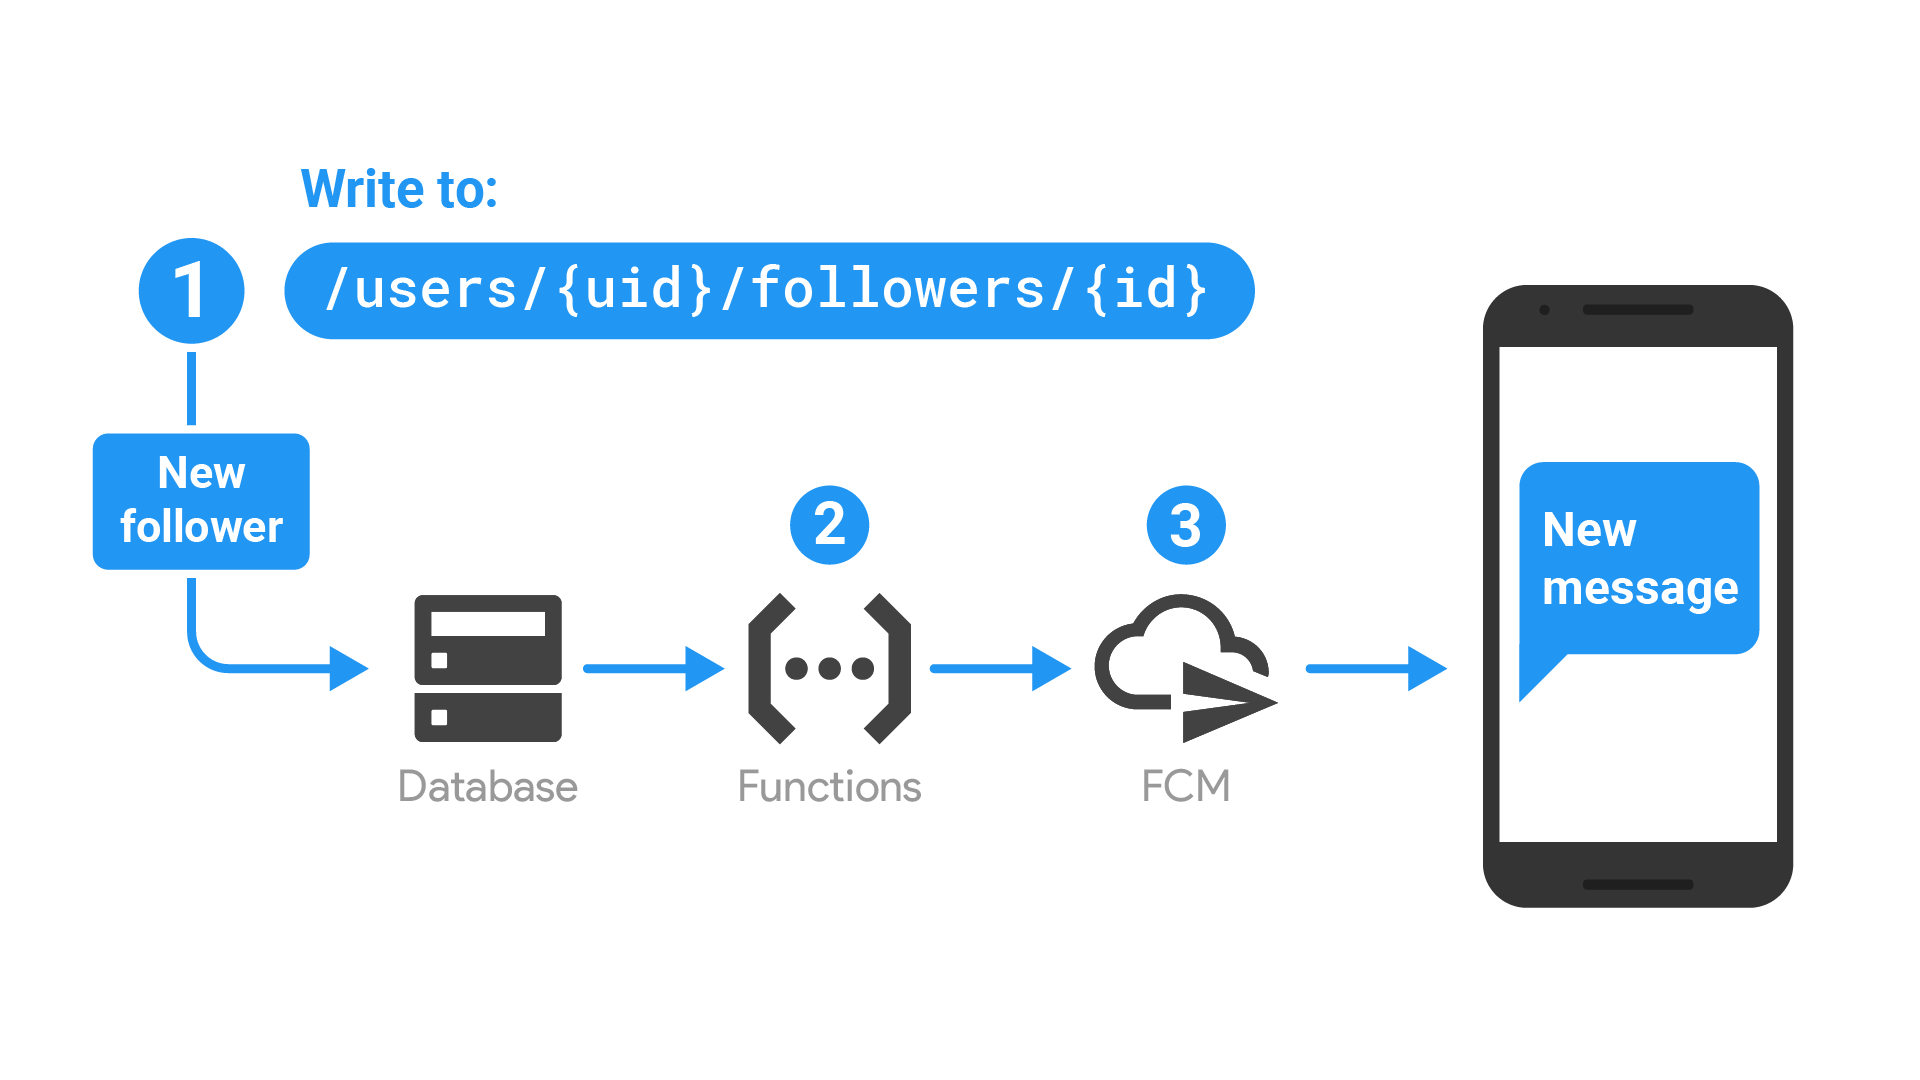
\includegraphics[scale=0.2]{images/firebase_functions_notify.png}
	\end{center}
	\caption{Cloud Functions Anwendungsfall Benachrichtigung}
	\label{fig:functions_notifications}
\end{figure}
In Abbildung \ref{fig:functions_notifications} ist ein typischer Anwendungsfall beschrieben. 
Ein Event auf der Datenbank wird ausgelöst, hier ein neuer Nutzer folgt einem weiteren Nutzer.
Es wird also ein Dokument in der Unter-Sammlung \texttt{followers} erzeugt. Diese Unter-Sammlung befindet sich innerhalb des Dokumentes \texttt{uid} der Sammlung \texttt{users}.
Im zweiten Schritt erstellt die Funktion eine Nachricht, welche über Firebase Cloud Messaging (FCM) versendet werden soll.
Über abgespeicherte Tokens sendet FCM die Benachrichtigung an das Gerät des Nuters \texttt{uid}.\cite{firebase2021}
\subsubsection{Cloud Messaging}
Firebase Cloud Messaging ist eine plattformübergreifende Messaging-Lösung zum zuverlässigen Versenden von Nachrichten an Nutzergeräte.
In Abbildung \ref{fig:cloudmessaging_architecture} ist die Architektur dieses Tools dargestellt.
Hierbei wird es grundlegend in das Erstellen, Transportieren und Empfangen der Nachrichten unterteilt.\cite{firebase2021}\\
\begin{itemize}
	\item \textbf{Erstellen} Die zu versendenden Nachrichten können, wie in Kapitel \ref{sec:cloudfunctions} beschrieben, manuell oder automatisiert erzeugt werden. 
	Bei der Automatisierung ist wichtig, dass die Nachrichten in einer vertrauenswürdigen Serverumgebung erstellt werden, damit alle Nachrichtentypen unterstützt werden (Schritt 1). 
	Das FCM Backend akzeptiert dann in Schritt 2 Nachrichtenanfragen, ordnet die Nachrichten verschiedenen Themen zu und erzeugt unter anderem Metadaten für Nachrichten, wie bspw. die Nachricht ID. 
	\item \textbf{Transportieren} Die Nachrichten werden hierbei an die entsprechenden Geräte weitergeleitet.
	Da verschiedene Geräte auf unterschiedlichen Plattformen basieren, muss die Transportschicht auf Plattformebene arbeiten.
	Hierfür werden folgende Ebenen genutzt:
	\begin{itemize}
		\item Android Transport Layer (ATL) für Android-Geräte mit Google Play-Diensten
		\item Apple Push Notification Service (APNs) für iOS-Geräte
		\item Web-Push-Protokoll für Web-Apps
	\end{itemize}
	\item \textbf{Empfangen} Das FCM SDK behandelt die Benachrichtigung oder Nachricht. Dies ist abhängig vom Vorder-/ Hintergrundstatus der Anwendung und der jeweiligen Anwendungslogik.
\end{itemize}


\begin{figure}[htb]
	\begin{center}
		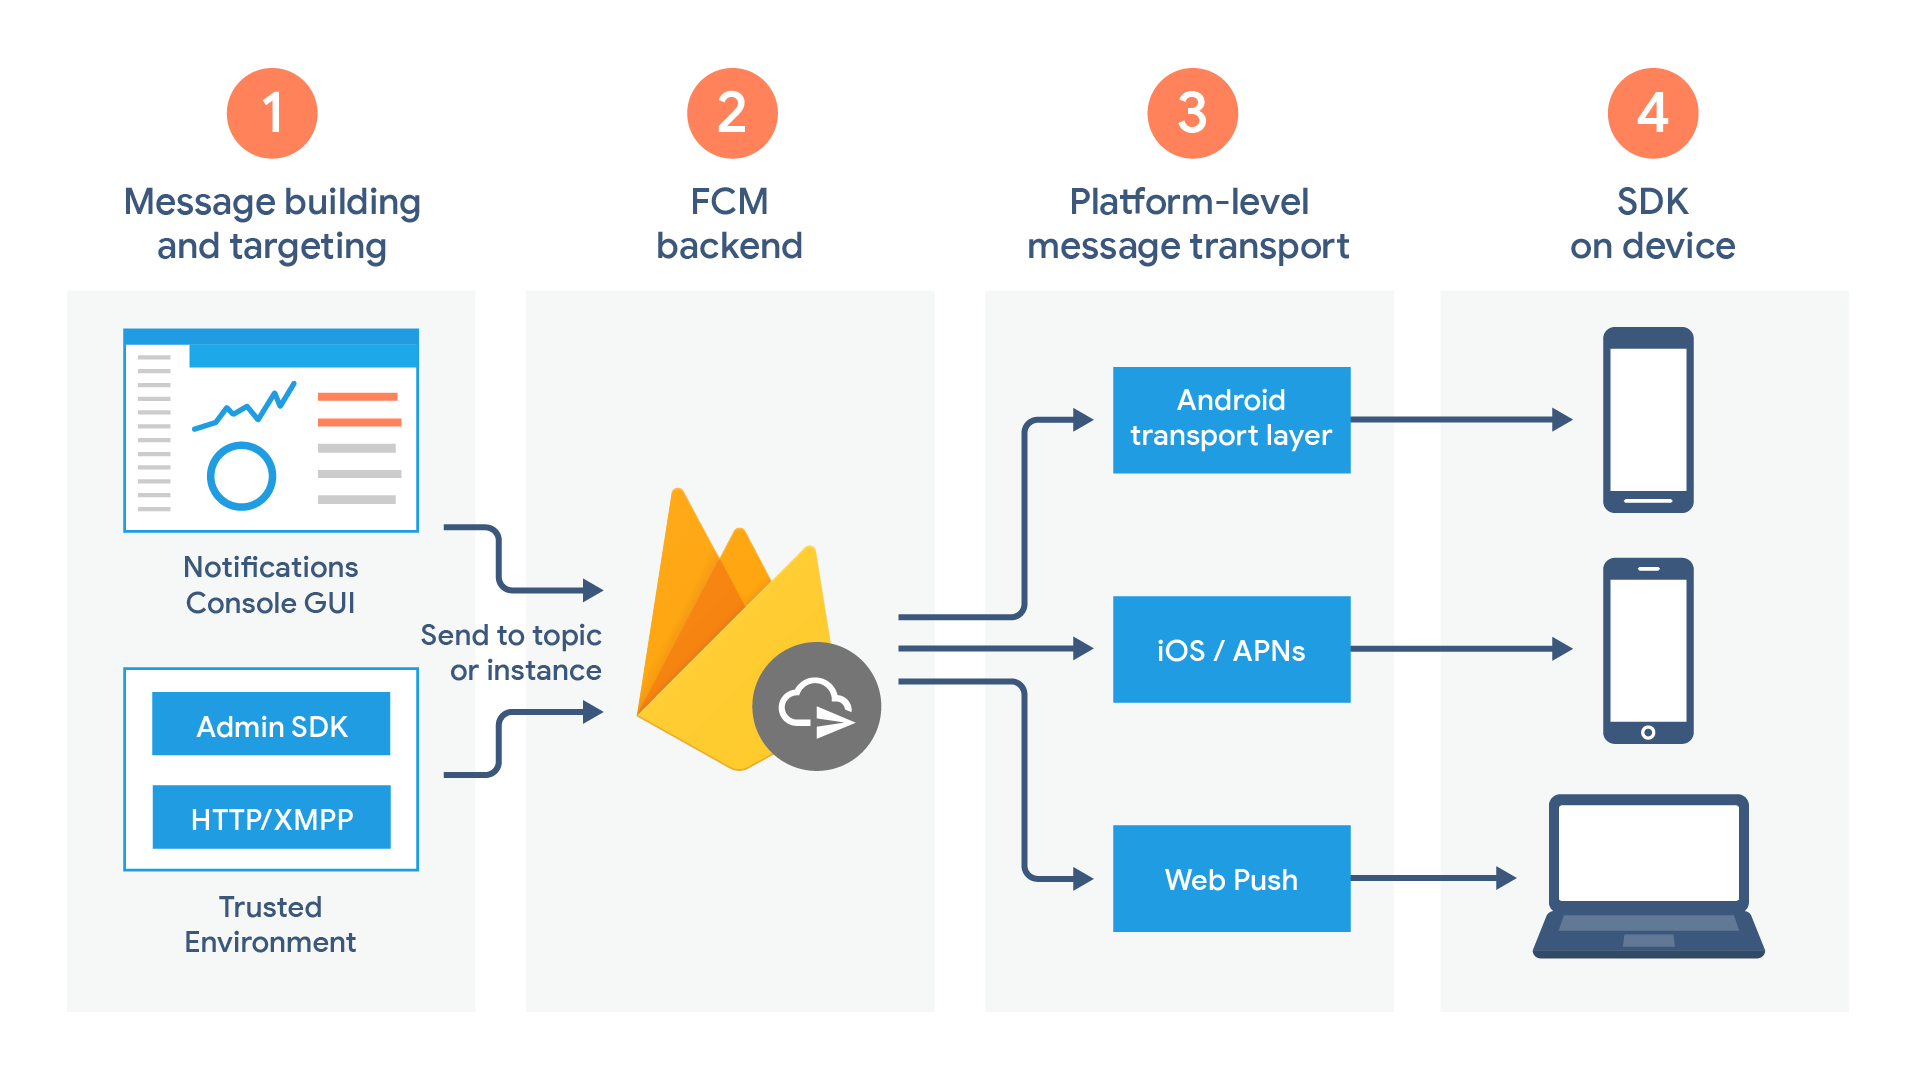
\includegraphics[scale=0.23]{images/firebase_cloudmessaging_architecture.png}
	\end{center}
	\caption{Firebase Cloud Messaging Architektur}
	\label{fig:cloudmessaging_architecture}
\end{figure}

\subsubsection{Google AdMob}
Google AdMob bietet eine einfache Art, gezielte Werbung innerhalb der Anwendung zu schalten und somit die Anwendung zu monetarisieren.
Zusätzlich bietet das Tool in Kombination mit Google Analytics\footnote{Ein freies Analysetool, welches über alle Tools hinweg Ereignisse sammelt und diese Werte direkt graphisch darstellt. Da es für die Implementierung nicht weiter relevant ist, wird es nicht detaillierter besprochen. Zusätzliche Informationen unter \href{https://firebase.google.com/docs/analytics}{firebase.google.com}.} zusätzliche Anwendungsdaten und Analysefähigkeiten.\\
Werbung lässt sich in unterschiedlicher Weise anzeigen (siehe Abbildung \ref{fig:firebase_admob})und lässt sich reibungslos in UI Komponenten integrieren. 
Verschiedene Features sind hier jedoch plattformabhängig. 
Auf der Android Plattform ist es für Nutzer möglich, beworbene Produkte direkt aus der Anwendung heraus zu kaufen.\\
Ein weiteres Werbetool \textit{Google Mobile Ads SDK} ist eine alleinstehende SDK, hingegen Google AdMob bietet einfache Integration in Firebase und weitere Tools.\cite{firebase2021}

\begin{figure}[htb]
	\begin{center}
		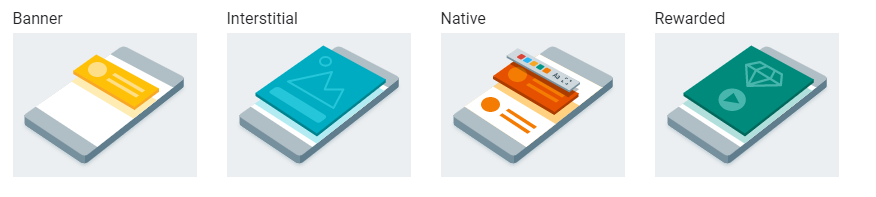
\includegraphics[scale=0.55]{images/firebase_admob_ads.PNG}
	\end{center}
	\caption{Google AdMob Anzeigemöglichkeiten}
	\label{fig:firebase_admob}
\end{figure}






































\subsection{Recommendationssystem}
%Auf der Webseite Youtube allein werden minütlich mehr als 500 Stunden Videomaterial hochgeladen. (\url{https://blog.youtube/press/}, 10.02.2021)
Um bei einer solch unvorstellbaren Menge an Daten (allein auf einer Webseite) den Überblick als Endnutzer behalten zu können, ist ein personalisierten Filtersystems unausweichlich.

\noindent
Solche Filtersysteme, auch Recommendation System genannt, nutzt bisher gesammelte Daten um Nutzern potentiell interessante Objekte jeweils individuell vorzuschlagen.
Ein sogenannter \textit{Candidate Generator} ist hierbei ein Recommendation System, welches die Menge $M$ als Eingabe erhält und für jeden Nutzer eine Menge $N$ ausgibt. Hierbei umfasst $M$ alle Objekte und gleichzeitig gilt $N \subset M$. 

\noindent
Die Bestimmung einer solchen Menge $N$ beruht grundlegend auf zwei Informationsarten. Erstens die sogenannten Nutzer-Objekt Interaktionen, also beispielsweise Bewertungen oder auch Verhaltensmuster; Und zweitens die Attributwerte von jeweils Nutzer oder Item, also beispielsweise Vorlieben von Nutzern oder Eigenschaften von Items.\cite{aggarwal2016}
Systeme, welche zum Bewerten ersteres benutzen, werden \textit{collaborative filtering} Modelle genannt. Andere, welche zweiteres verwenden, werden \textit{content-based filtering} Modelle genannt. Wichtig hierbei ist jedoch, dass \textit{content-based filtering} Modelle ebenfalls Nutzer-Objekt Interaktionen (v.a. Bewertungen) verwenden können, jedoch bezieht sich dieses Modell nur auf einzelne Nutzer - \textit{collaborative filtering} basiert auf Verhaltensmustern von allen Nutzern bzw. allen Objekten.

\noindent
Ein solches Recommendation System kann im einfachsten Fall wie in \ref{Recommendation Matrix} als Matrix dargestellt werden.

\begin{table}[tbt]
	\caption{Nutzer-Item Matrix mit Bewertungen. Jede Zelle $r_{u;i}$ steht hierbei für die Bewertung des Nutzers $u$ an der Stelle $i$}
	\centering
	\label{Recommendation Matrix}
	\begin{tabular}{lcllllll}
		& \multicolumn{7}{c}{Items}                                                                                                                                                        \\
		& \multicolumn{1}{l}{}     & \multicolumn{1}{c}{1}  & \multicolumn{1}{c}{2}  & \multicolumn{1}{c}{...} & \multicolumn{1}{c}{i}  & \multicolumn{1}{c}{...} & \multicolumn{1}{c}{m}  \\ \cline{3-8} 
		& \multicolumn{1}{c|}{1}   & \multicolumn{1}{l|}{2} & \multicolumn{1}{l|}{}  & \multicolumn{1}{l|}{1}  & \multicolumn{1}{l|}{}  & \multicolumn{1}{l|}{}   & \multicolumn{1}{l|}{3} \\ \cline{3-8} 
		Users & \multicolumn{1}{c|}{2}   & \multicolumn{1}{l|}{4} & \multicolumn{1}{l|}{}  & \multicolumn{1}{l|}{}   & \multicolumn{1}{l|}{5} & \multicolumn{1}{l|}{}   & \multicolumn{1}{l|}{}  \\ \cline{3-8} 
		& \multicolumn{1}{c|}{...} & \multicolumn{1}{l|}{}  & \multicolumn{1}{l|}{}  & \multicolumn{1}{l|}{1}  & \multicolumn{1}{l|}{}  & \multicolumn{1}{l|}{}   & \multicolumn{1}{l|}{4} \\ \cline{3-8} 
		& \multicolumn{1}{c|}{u}   & \multicolumn{1}{l|}{}  & \multicolumn{1}{l|}{4} & \multicolumn{1}{l|}{}   & \multicolumn{1}{l|}{5} & \multicolumn{1}{l|}{}   & \multicolumn{1}{l|}{1} \\ \cline{3-8} 
		& \multicolumn{1}{l|}{}    & \multicolumn{1}{l|}{2} & \multicolumn{1}{l|}{}  & \multicolumn{1}{l|}{}   & \multicolumn{1}{l|}{}  & \multicolumn{1}{l|}{3}  & \multicolumn{1}{l|}{}  \\ \cline{3-8} 
		& \multicolumn{1}{l|}{n}   & \multicolumn{1}{l|}{}  & \multicolumn{1}{l|}{4} & \multicolumn{1}{l|}{}   & \multicolumn{1}{l|}{3} & \multicolumn{1}{l|}{}   & \multicolumn{1}{l|}{}  \\ \cline{3-8} 
	\end{tabular}
\end{table}

\subsubsection{Nutzerinformation}
Damit ein \textit{Recommender System} einem Nutzer Vorschläge bereitstellen kann, benötigt es Nutzerinformationen. Das Design des jeweiligen Systems hängt auch, wie oben beschrieben, von der Art der Information und von der Art der Beschaffung dieser ab.

\paragraph{Explizite Nutzerinformation}
Bei der expliziten Methode muss der Nutzer individuelle Informationen aktiv über sich preisgeben. Dies kann über konkrete Fragestellungen zu beispielsweise Geburtsdatum, Geschlecht oder Interessen geschehen. Diese Art der Information beschreiben einen Nutzer konkret. 

\noindent
Eine andere Art der Information sind Bewertungen von Objekten. Diese lassen sich beispielsweise Intervall basiert darstellen. Hierbei werden geordnete Zahlen in einem Intervall als Indikator genutzt, ob ein Objekt gut oder schlecht war - zum Beispiel eine Bewertung eines Produktes von 0 bis 5 Sternen bei Amazon. Diese Information beschreiben die Vorlieben eines Nutzers konkret.

\noindent
Je größer diese Skala ist, desto differenzierter ist auch das Meinungsbild, da jeder Nutzer sich genau ausdrücken kann. Jedoch desto komplizierter und unübersichtlich wird auch das Bewertungsverfahren an sich, da man einen zu großen Entscheidungsraum für den Nutzer darbietet.

\paragraph{Implizite Nutzerinformation}
Um implizit Nutzerinformationen zu erfassen, muss ein System die Verhaltensmuster seiner Kunden als Daten abspeichern. Beispielsweise könnte das System von YouTube erfassen, ob Videos frühzeitig abgebrochen oder ganz angeschaut werden. Anklicken von Webseiten und die darauf verbrachte Zeit könnte ebenfalls als Bewertung gespeichert und zur Generierung von Vorschlägen genutzt werden.

\subsubsection{Content-based filtering}
Unter \textit{content-based filtering} versteht man das Betrachten von Ähnlichkeiten zwischen Objekten anhand von Schlüsselwörtern (Eigenschaften) und daraus dann das Vorhersagen der Nutzer-Objekt Kombination für ein bestimmtes Objekt. 
Nimmt man an, Film 1 und Film 2 haben ähnliche Eigenschaften (gleiches Genre, gleiche Schauspieler, ...) und Nutzer A mag Film 1, so wird das System Film 2 vorschlagen.

\noindent
Das System ist also unabhängig von anderen Nutzerdaten, da die Vorschläge nur auf Präferenzen eines einzelnen Nutzers basieren. Dies bietet im Hinblick auf eine App auch gute Skalierungs"-möglich"-keiten. Zudem kann auf Nischen-Präferenzen gut eingegangen werden, da nicht mit anderen Nutzerdaten verglichen wird, sondern nur ein Nutzer für sich betrachtet wird.

\noindent
Gleichzeitig schlagen \textit{content-based filtering} Systeme aber eher offensichtliche Objekte vor, da Nutzer oft unzureichend genaue "Beschreibungen", also Vorlieben mit sich bringen. Dadurch, dass nur basierend auf Schlüsselwörter neue Objekte vorgeschlagen und andere Nutzerwertungen nicht miteinbezogen werden, sind die Vorschläge sehr wahrscheinlich oftmals ähnlich bis gleich - man "verfängt" sich quasi in eine Richtung.\cite{aggarwal2016}

\subsubsection{Collaborative Filtering}
Unter \textit{collaborative filtering} versteht man das Betrachten von Ähnlichkeiten im Verhalten von Nutzern anhand von Bewertungen und Prä"-fer"-enzen, bzw. anhand der Ähn"-lich"-keiten von Objekten.

\noindent
Generell unterscheidet man in zwei Typen:\cite{aggarwal2016}

\begin{enumerate}		
	\item \textit{Memory-based Methoden}: Es wird, wie oben beschrieben, aus gesammelten Daten Ähn"-lich"-keit herausgearbeitet und Nutzer-Objekt Kombinationen durch eben diese vorhergesagt. Daher wird dieser Typ auch \textit{neighborhood-based collaborative filtering} genannt. Man unterscheidet weiter in:
	\begin{enumerate}
		\item \textit{User-based}: Ausgehend von einem Nutzer A werden andere Nutzer mit ähnlichen Nutzer-Objekt Kombinationen gesucht, um Vorhersagen für Bewertungen von A zu treffen. Ähnlichkeitsbeziehungen werden also über die Reihen der Bewertungsmatrix berechnet.
		\item \textit{Item-based}: Hierbei werden ähnliche Objekte gesucht und diese genutzt um die Bewertung eines Nutzers für ein Objekt vorherzusagen. Es werden somit Spalten für die Berechnung der Ähnlichkeitsbeziehungen verwendet.
	\end{enumerate}
	\item \textit{Model-based Methoden}: Machine Learning und Data Mining Methoden werden verwendet um Vorhersagen über Nutzer-Objekt Kombinationen zu treffen. Hierbei sind auch gute Vorhersagen bei niedriger Bewertungsdichte in der Matrix möglich.
\end{enumerate}

\noindent
Vereinfacht gesagt: Wenn Nutzer A ähnliche Bewertungen verteilt wie Nutzer B, und B den Film 1 positiv bewertet hat, wird das System Film 1 auch Nutzer A vorschlagen. Das selbe gilt auch umgekehrt (\textit{Item-based}).

\noindent
Diese Art leidet sehr unter dem \textit{sparsity} Problem, also dass die Nutzer zu wenige Bewertungen von Objekten ausüben. Daher sind Vorhersagen über Ähnlichkeit von Nutzern aufgrund unzureichender Datensätze nicht sinnvoll möglich. Dieses Problem wird \textit{Cold-Start Problem} genannt.

\subsubsection{Ähnlichkeit von Objekten und Nutzern}
Sowohl bei \textit{collaborative filtering}, als auch bei \textit{content-based filtering} wird jedes Objekt und jeder Nutzer als ein Vektor im Vektorraum-Modell $E = \mathbb{R}^d$ (englisch \textit{embedding space}) erfasst. Sind Objekte beispielsweise ähnlich, haben sie eine geringe Distanz voneinander. 

\noindent
Ähnlichkeitsfunktionen sind Funktionen $s : E \times E  \rightarrow \mathbb{R}$ welche aus zwei Vektoren beispielsweise von einem Objekt $q \in E$ und einem Nutzer $x \in E$ ein Skalar berechnen, welches die Ähnlichkeit dieser zwei beschreibt $s(q,x)$.

\noindent
Hierfür werden mindestens eine der folgenden Funktionen verwendet:
\begin{itemize}
	\item Cosinus-Funktion
	\item Skalarprodukt
	\item Euklidischer Abstand
\end{itemize} 

\paragraph{Cosinus-Funktion}
Hier wird einfach der Winkel zwischen beiden Vektoren berechnet: $s(q,x) = \cos(q,x)$

\paragraph{Skalarprodukt}
Je größer das Skalarprodukt, desto ähnlicher sind sich die Vektoren. $s(q,x) = q \circ x = \sum_{i=1}^{d}q_i x_i$ 

\paragraph{Euklidischer Abstand}
$s(q,x) = ||q-x|| = [\sum_{i=1}^{d}(q_i - x_i)^2]^\frac{1}{2}$





\url{https://dl.acm.org/doi/pdf/10.1145/3383313.3412488}
\url{http://www.microlinkcolleges.net/elib/files/undergraduate/Photography/504703.pdf}	
		

\section[Konzept]{Konzept? \hfill \normalfont \small{Autor-Name}}
\section[Funktionen/Komponenten]{Funktionen/Komponenten \hfill \normalfont \small{Autor-Name}}

\subsection{Swipe/Aussuchen/Voting}		

\subsection{Matches/Chat}		

\subsection{Film-/Serienvorschläge}		

\subsection{Gruppenorgien}		

\subsection{Gespeicherte Filme/Filmliste}		

\subsection{Barrierefreiheit}
\label{sec:barrierefreiheit}

Barrierefreiheit im Allgemeinen bedeutet, dass ein Gegenstand, eine Einrichtung oder Informationsquelle für Menschen mit Behinderung ohne Unzulänglichkeiten nutzbar, zugänglich oder auffindbar ist (\cite{behindertengleichstellungsgesetz}, §4). In der Softwareentwicklung versteht man darunter Applikationen für Menschen mit Einschränkungen zugänglich und bedienbar zu machen. Bezogen auf die Entwicklung von  mobilen Apps gilt es dabei den akustischen, optischen oder motorischen Einschränkungen der Benutzer entgegenzuwirken. \\


\subsubsection{Barrierefreiheit in mobilen Anwendungen}
Mit der Verbreitung von Smartphones ist die Benutzung mobiler Apps stark angestiegen und mittlerweile in nahezu jedem Haushalt aufzufinden. Obwohl etwa 9,5\% aller in Deutschland lebenden Menschen einen Schwerbehindertenausweis besitzen (Stand 24. Juni 2020)\cite{schwerbehindertenausweis} was etwa 7,9 Millionen Menschen entspricht, ist die Implementierung von barrierefreier Bedienung nicht selbstverständlich. Gerade Programmierern/innen aus dem privaten Sektor sind diese Funktionen oft nicht bekannt, es besteht kein Interesse oder sie werden schlichtweg vergessen. Software, die für öffentliche Einrichtungen entwickelt wird, ist durch das Behindertengleichstellungsgesetz von 2002 dazu verpflichtet ihr Softwareangebot bis spätestens dem 23. Juni 2021 barrierefrei zu gestalten (\cite{behindertengleichstellungsgesetz}, §12a Abs.1). Hierzu zählen sämtliche Webseiten sowie mobile Anwendungen. \\


\subsubsection{Barrierefreiheit in Filmen und Serien}
Auch die Zugänglichkeit von Filmen und Serien für Menschen mit eingeschränkter Wahrnehmung wurde in den letzten Jahren stark verbessert. 
Hierbei lässt sich zwischen optischer und akustischer Einschränkung differenzieren. Für hörgeschädigte Personen werden bereits seit mehreren Jahrzehnten Untertitel eingesetzt. Was früher für vereinzelte Filme durch eine Funktion des Teletextes erreicht wurde, wird heutzutage durch eine integrierte Funktion des Videoplayers verwirklicht. Immer mehr Videos werden mit Untertiteln veröffentlicht. Manche Anbieter wie beispielsweise die Internetplattform YouTube bieten durch Spracherkennung automatisch generierte Untertitel an, was eine flächendeckende Untertitelung ermöglicht.\\
Auch für Menschen mit eingeschränktem Sehvermögen werden Filme und Serien mithilfe von Audiodeskriptionen vermehrt zugänglich gemacht. Hierbei wird die bereits vorhandene Tonspur mit Bildbeschreibungen und Kommentaren versehen. Was bis vor wenigen Jahren noch etwas Besonderes war und nur für ausgewählte Filme bestimmt war, ist heutzutage Standard. Größere Video-On-Demand-Plattformen wie Netflix oder Amazon Prime bieten diese Möglichkeit bei nahezu allen Eigenproduktionen an. Zusätzlich werden bestehende Filme neu mit Audiodeskriptionen versehen.\\


\noindent Hieraus lässt sich leicht erkennen, dass Filme und Serien heutzutage auch von Menschen mit Einschränkungen genutzt werden. Was auf den ersten Blick vielleicht nicht bedacht wird oder als  unwichtig abgestempelt wird, kann einen nicht unerheblichen Vergrößerungsfaktor für den Kundenstamm bewirken. Für die Entwicklung einer mobilen App, bei der Filme und Serien bewertet werden, spielt also die Barrierefreiheit eine wichtige Rolle und darf auf keinen Fall vernachlässigt werden. 


\subsubsection{Barrierefreiheit bei StreamSwipe}
\label{sec:bf-streamswipe}

Bei der Entwicklung von StreamSwipe werden mehrere mögliche Einschränkungen der Nutzer betrachtet und entsprechend reagiert. Ziel ist es, dass sowohl der Kunde sowie der Anbieter maximal davon profitieren. Hierfür soll die App für ein möglichst großes Publikum zugänglich gemacht werden, jedoch auch sogenanntes Over-Engineering vermieden werden, da zu viele Funktionen eine App unübersichtlich, teuer und langsamer werden lassen.\\

\noindent
Allgemein wird Leserlichkeit durch große Schriftgrößen, hohe Farbkontraste, große Schaltflächen oder universelles Design erreicht. Alleine in Deutschland tragen 44,5 Millionen Menschen regelmäßig eine Brille oder Kontaktlinsen und benötigen somit Sehhilfen \cite{sehhilfen}. Unterstützung auf Seiten der App kann hierfür durch vergrößerbaren Text geschehen. Da aber davon ausgegangen werden kann, dass Personen, die sich auf Sehhilfen verlassen, bereits eine Brille oder Kontaktlinsen besitzen, wird die Textgröße vorerst nicht variabel gehalten. Außerdem gibt es bei Android- und Apple-Smartphones bereits eingebaute Vergrößerungsfeatures, die Bildausschnitte vergrößert darstellen können. Aus diesem Grund wird in diesem Projekt kein Fokus auf dieses Feature gelegt. \\
Farbblindheit kann jedoch in vielen Formen auftreten. Um der bekannten Farbfehlsicht entgegenzuwirken, werden Farben aus Problembereichen wie Rot und Grün nicht nebeneinander benutzt. Allgemein wird ein schlichtes Design gewählt und Farben nur zu Akzentuierung und als Stilmittel benutzt (vgl. Abbildungen \ref{fig:BF-Beispiele}), statt als Informationsträger.  Geringe Sehschärfe durch Achromatopsie kann wie weiter oben beschrieben umgangen werden.\\


\begin{figure}[tbt]
	\begin{subfigure}{0.5\textwidth}
	\centering
	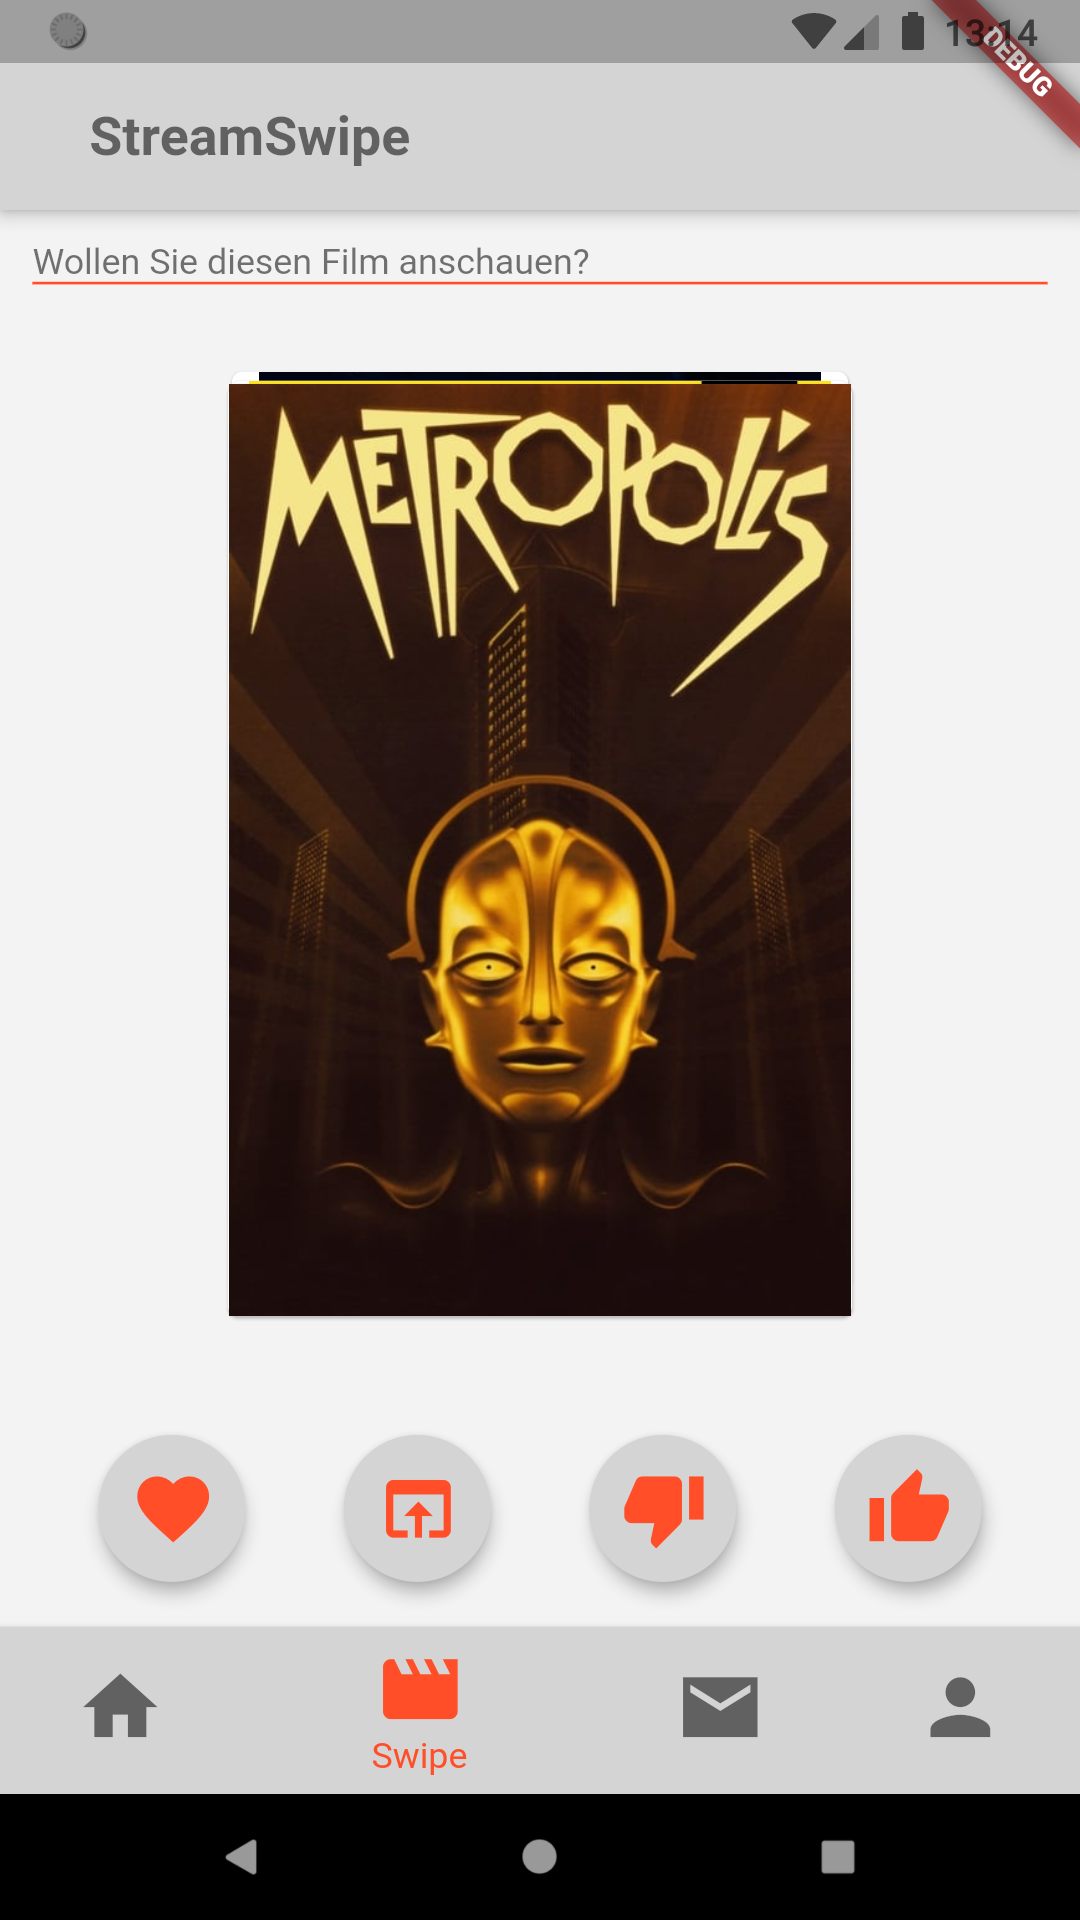
\includegraphics[scale=0.15]{Barrierefreiheit/images/bsp-swipe.png}
	\caption{}
	\label{fig:bf-beispiel_a}
	\end{subfigure}
	\begin{subfigure}{0.5\textwidth}
	\centering
	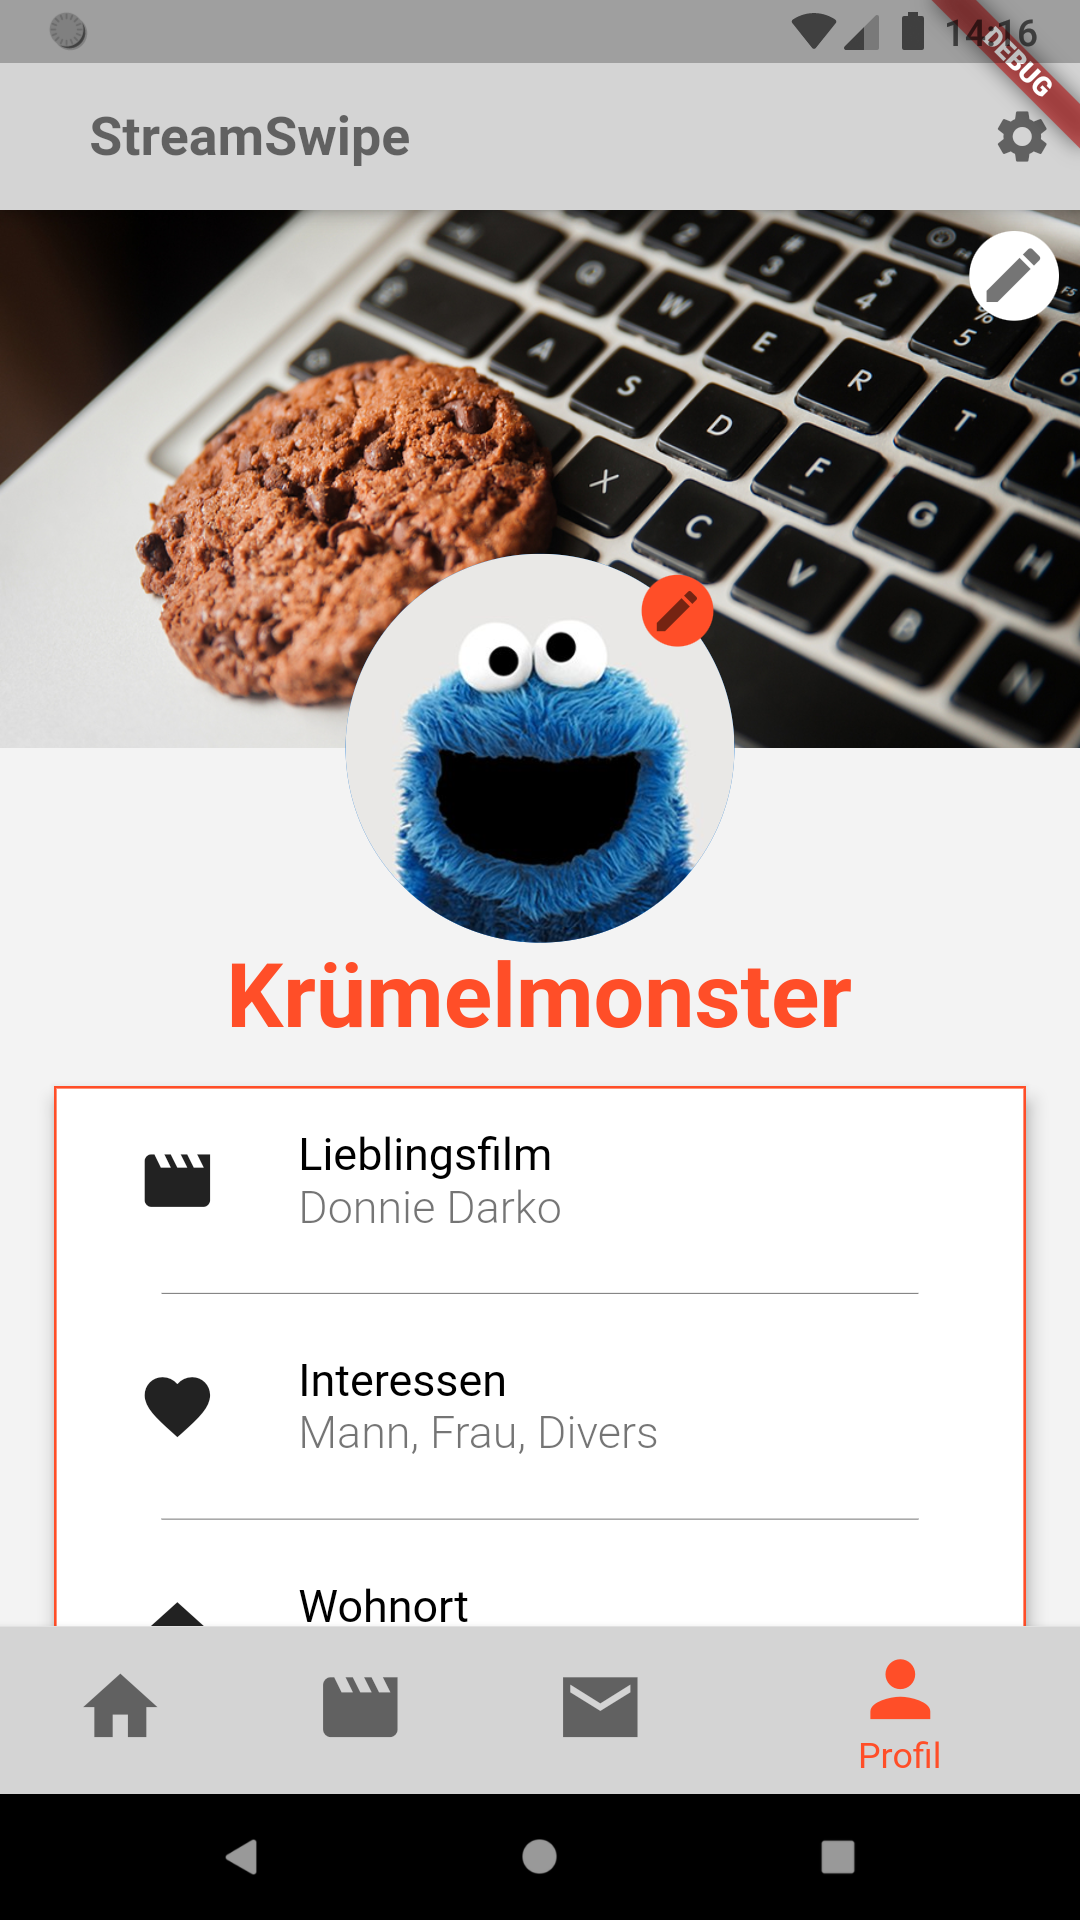
\includegraphics[scale=0.15]{Barrierefreiheit/images/bsp-profil.png}
	\caption{}
	\label{fig:bf-beispiel_b}
	\end{subfigure}
\caption[Screenshots als Beispiele für Barrierefreiheit]{Screenshots aus der App StreamSwipe als Beispiele zu (a) schlichtem Design, bei dem farbige Akzente nicht der Informationenübertragung dienen um die Zugänglichkeit für farbblinde Menschen zu verbessern und für einen Icon in (b), welcher sonst durch sehgeschädigte Menschen nicht wahrnehmbar ist, wird exemplarisch eine Semantik implementiert.}
\label{fig:BF-Beispiele}
\end{figure}


\noindent
Ist die Sehkraft noch weiter eingeschränkt oder gar nicht mehr vorhanden, werden Semantiken eingesetzt. Hierbei erhält jedes Element auf dem Bildschirm eine Beschreibung, die vorgelesen werden kann. Bei Zahlen und Texten werden diese vorgelesen, sofern keine weitere Information hinterlegt ist. Besonders hilfreich ist dies jedoch bei Abbildungen. Ausgeführt wird das Auslesen von einem Screenreader. Mobile Geräte haben diese Funktion bereits standardmäßig eingebaut (VoiceOver bei Apple und TalkBack bei Android) und wandeln die Semantiken mittels Sprachsynthese in akustische Signale um. Bei Desktopanwendungen wie z.B. JAWS für Windows können diese Informationen zusätzlich auch durch eine Braillezeile wiedergegeben werden.\\
Bei Flutter ist das Hinzufügen von Semantiken bereits eingebaut. Hierfür kann ein String dem jeweiligen Bereich zugeordnet werden. In Beispiel \ref{lst:semantics} ist hierfür der Code des Buttons, der zu den Einstellungen führt. In Abbildung \ref{fig:bf-beispiel_b} ist dieser Button ganz rechts oben im Eck zu sehen.\\
Die Funktion \texttt{GestureDetector()} erkennt Interaktionen mit dem Touchscreen, wobei hier nur auf Antippen reagieren soll, deshalb die Funktion \texttt{onTap:()$\{\}$}, die auf den Einstellungsbildschirm leitet. Diese Implementierung ist hier aber nicht von Relevanz und wird übersprungen. In dem \texttt{GestureDetector()} ist ein Icon eingebettet, von der Form \textit{Settings}, was einem Zahnrad entspricht. Dieses Icon erhält eine Farbe und anschließend eine Semantik aus allem was in den Anführungszeichen steht. Ein Screenreader kann AE erkennen und ihn als den Umlaut Ä aussprechen. \\
So wird im kompletten Programm für jedes relevante Element vorgegangen. Teilweise  müssen den Semantiken Variablen übergeben werden, da sich die vorzulesende Information ändert wie beispielsweise bei den Filmtiteln.
    
\begin{lstlisting}[caption=Codeausschnitt in Dart von einem Button mit Semantiken.,label=lst:semantics]
GestureDetector(
  onTap: () {
     ...
  },
  child: Icon(
    Icons.settings,
    color: Provider.of(context).colors.textSmall,
    semanticLabel: "Einstellungen. Zum Auswaehlen doppeltippen.",
  )
),
\end{lstlisting}

\noindent
Bei einer sauberen Implementierung wird auf diese Weise vorgegangen und eine bereits vorhandene Funktion verwendet. Dies vereinfacht nicht nur die Leserlichkeit des Codes, sondern bietet auch die höchste Modularität, da hierbei normalerweise standardisierte Schnittstellen für Betriebssysteme oder andere Anwendungen verwendet werden. In diesem Fall  müssen die Screenreader von Android und Apple damit arbeiten können.\\

\noindent 
Um für Personen mit eingeschränktem Hörvermögen oder vollständiger Gehörlosigkeit die App zugänglich zu machen, wird auf akustisches Feedback als notwendige Infor"-mations"-über"-tragung verzichtet. Innerhalb der App werden keine Geräusche erzeugt, außer der oben beschriebenen Funktion der Semantiken. Beim Erhalten einer neuen Nachricht oder eines neuen Matches kann weiterhin optional eine akustische Benachrichtigung erhalten werden. Hierbei wird die betriebssystemeigene Funktion übernommen, sodass in der App keine neuen Einstellungen vorgenommen werden müssen.\\

\noindent
Auch feinmotorische Einschränkungen werden versucht zu umgehen. Die Navigation und die Filmbewertung in StreamSwipe können durch großflächige Wischbewegungen ausgeführt werden. Wo diese Lösung nicht möglich ist, werden verhältnismäßig große Buttons eingesetzt. Lediglich beim Registrieren und Einloggen werden feine Bewegungen erfordert. Hierbei öffnet sich allerdings die als Standard eingestellte digitale Tastatur, die in vielen Fällen eine Spracheingabe besitzt, sodass die sehr kleinen Tasten nicht benutzt werden müssen.\\

%TODO Diesen Satz evtl. ganz ans Ende ins Fazit
\noindent
Sollte sich in Zukunft jedoch Kritik in Form von negativen Nutzerbewertungen herauskristallisieren, kann eines der noch nicht implementierten Features über ein Update nachgerüstet werden.


\section[Benutzeroberflächen]{Benutzeroberflächen \hfill \normalfont \small{Vincent Schreck}}
Die Benutzeroberfläche einer Software muss im Grunde genommen nur einen Informationsfluss in zwei Richtungen erzeugen. Die eine Richtung liefert Informationen an den User und über die andere kann der User Informationen an das System weitergeben. Um auf dem heutigen Markt Fuß fassen zu können, sollte eine Oberfläche jedoch wesentlich mehr Aspekte erfüllen. 




\subsection{Aspekte von Benutzeroberflächen}
\label{sec:UI-Aspekte}
Die Vielschichtigkeit einer Benutzeroberfläche kann ausschlaggebend für den Erfolg einer Applikation sein, abhängig davon welche Erfahrungen der User mit der Oberfläche macht und welche Eindrücke sie hinterlässt. Hieraus resultiert wie lange ein User auf der App bleibt und wie oft er zurück kommt. Neben der Nutzungszeit erhöht eine positive User Experience die Weiterempfehlungsrate.\\
Bei erfolgreicher Software besteht ein großer Teil der Entwicklung in der Planung der Oberfläche, da die User Experience nicht zu umgehen ist. Auf die eine oder andere Art erlebt der User immer eine Erfahrung. Neben den offensichtlichen Aus- und Eingabefunktionen werden beispielsweise folgende Kriterien  betrachtet:\\

\noindent
\hangindent1cm
\textbf{Simpel:} Ausgegebene Information kann zum Beispiel durch Icons, Farben oder Symbole vereinfacht werden. Eine Oberfläche sollte weder überladen sein, noch sollten alle Ein- und Ausgaben auf verschiedenen Screens verteilt sein. Bei der Entwicklung wird eine gesunde Mischung aus maximaler Funktionalität und einfacher, übersichtlicher Darstellung angestrebt.\\

\noindent
\hangindent1cm
\textbf{Einheitlich:} Die Bedienung und das Lesen von Applikationen kann erheblich vereinfacht werden wenn einheitliche Bedien- oder Ausgabeelemente verwendet werden. Nicht nur innerhalb einer App ist es sinnvoll konsistente Elemente in der Oberfläche zu verwenden, auch Funktionen von anderen Apps können die Bedienung vereinfachen. Bekannte Funktionen bei Smartphone-Applikationen sind zum Beispiel die Vergrößerung mit zwei Fingern oder das \glqq Daumen nach oben\grqq -Symbol als positive Rückmeldung. Durch das  Einbauen solcher Features wird eine App intuitiv und ohne Einführung bedienbar.\\

\noindent
\hangindent1cm
\textbf{Benutzergesteuert:} Alle ausgeführten Aktionen sollten vom Benutzer ausgehen. Ein gutes Interface unterstützt den User lediglich bei seiner Bedienung, schränkt ihn aber nicht ein. Mit der heutigen Technologie ist die Verführung groß viele Funktionen automatisch ablaufen zu lassen. Was eigentlich der Sinn einer Applikation ist, kann jedoch auch negative Folgen haben. Zu viel Automatisierung verursacht das Gefühl von Kontrollverlust und Unsicherheit, was sich negativ auf das Vertrauen und somit auf die Benutzungszeit von dem User auswirkt. \\

\noindent
\hangindent1cm
\textbf{Klarheit:} Eine mobile App muss ohne Anleitung bedienbar sein. Sobald Unklarheiten beim User entstehen und Funktionen oder Ausgaben nicht erkannt werden können, verliert die Anwendung auf dem freien Markt. \\
Der User sollte zu jeder Zeit wissen welche Optionen ihm zur Verfügung stehen und welche Folgen seine Aktionen haben. Besonders wichtig ist das Feedback infolge einer Aktion. Auch wenn diese Aspekte offensichtlich erscheinen, können sie bei der Entwicklung einer App leicht übersehen werden. Verwendet werden einfache und für den User bekannte Funktionen, wie die Beschriftung aller Buttons oder das haptische, akustische oder optische Feedback beim drücken einem dieser Buttons.\\

\noindent
\hangindent1cm
\textbf{Benutzerfreundlich/Barrierefreiheit:} Die Bedienung der App sollte für Menschen mit Einschränkungen im vollen Umfang möglich sein. In Abschnitt \ref{sec:barrierefreiheit} wird auf dieses Thema tiefer eingegangen. Aber auch Benutzer ohne Einschränkungen erwarten eine einfache und übersichtliche Bedienung, die auch beispielsweise  Eingabefehler mit mehreren Versuchen verzeiht.\\

\noindent
\hangindent1cm
\textbf{Ästhetik:} Das Design spielt bei dieser Betrachtung gleich mehrere wichtige Rollen. Es sollte eine angenehme Arbeitsumgebung für den User erstellen, Ein- und Ausgaben verdeutlichen und gleichzeitig mithilfe eines eigenen Stils ein einzigartiges Image für die App schaffen (sogenanntes Branding) um deren Individualität und Wiedererkennungswert zu steigern. Das Design erschafft ein Erlebnis während der Benutzung und weckt Gefühle im User. \\

\noindent
Gerade weil viele dieser Aspekte unterbewusst wirken, ist eine ausgiebige Betrachtung unumgänglich.\\
Eine Schwierigkeit, die sich bei der Entwicklung ergibt sind die zwei unterschiedlichen Ziele. Einerseits sollten bestehende Design- und Bedienelemente  übernommen werden um die Bedienung intuitiv und übersichtlich zu gestalten, andererseits aber auch neue Ideen und Innovationen eingebracht werden, um sich von anderen Apps abzuheben und bleibenden Wiedererkennungswert aufzubauen.


\subsection{Oberflächen von StreamSwipe}
Die Smartphone-App lässt sich in mehrere Bereiche aufteilen, die sich in ihren Funktionen unterscheiden. Auf Basis der oben beschriebenen Grundlagen wurden diese Bereiche entworfen und werden in diesem Kapitel analysiert. Auch wenn manches davon als gewöhnlich oder naheliegend erscheint, so ist jedes Element mit Bedacht gewählt, erstellt und angepasst worden.

\subsubsection{Login-Screen}
\label{sec:loginscreen}
Bei erstmaliger Benutzung der App öffnet sich der Login-Screen. An diesem Punkt wird der erste Eindruck für den Benutzer gesetzt, wobei bei StreamSwipe ein schlichtes Design gewählt wurde. Man sieht helle Grautöne mit einem Akzentfarbton, welche sich durch alle Bildschirme der App ziehen werden. Abhängig davon, ob der User in den Systemeinstellungen den dunklen Modus gewählt hat, werden anstatt den hellen Grautönen, dunkle bis schwarze Farben dargestellt, siehe auch Abbildungen \ref{fig:homescreen_c} und \ref{fig:swipescreen_e}.\\
Auf dem Login-Screen (siehe Abbildung \ref{fig:login_a}) sind neben einer Überschrift mehrere beschriftete Textfelder und Buttons zu sehen, welche allesamt mit Semantiken versehen wurden, um durch einen Screenreader erkannt und identifiziert werden zu können. Die gewählte Anordnung wird universell bei Apps, Programmen und Webseiten benutzt, sodass die Felder auch ohne die eingetragenen Hinweistexte korrekt ausgefüllt werden könnten. Beim Antippen der Textfelder, öffnet sich die Standardtastatur des Betriebssystems. Sind alle Felder korrekt ausgefüllt, wird der User in die eigentliche App weitergeleitet, ansonsten wird durch individualisierte Fehlermeldung auf eventuelle Falscheingaben hingewiesen. Nach Erstellen eines neuen Accounts, durchläuft der User einen ähnlich aufgebauten Bildschirm (siehe Abbildung \ref{fig:login_b}) und wird danach aufgefordert weitere Informationen zur Profilvervollständigung einzugeben (siehe Abbildung \ref{fig:login_c} und \ref{fig:login_d}). Auch hierbei werden bekannte Bedienelemente wie Textfelder, Dropdownmenüs und Checkboxen verwendet, wie in den Abbildungen \ref{fig:login_e} und \ref{fig:login_f} beispielhaft dargestellt sind.


\begin{figure}[tbt]
	\begin{subfigure}{0.33\textwidth}
	\centering
	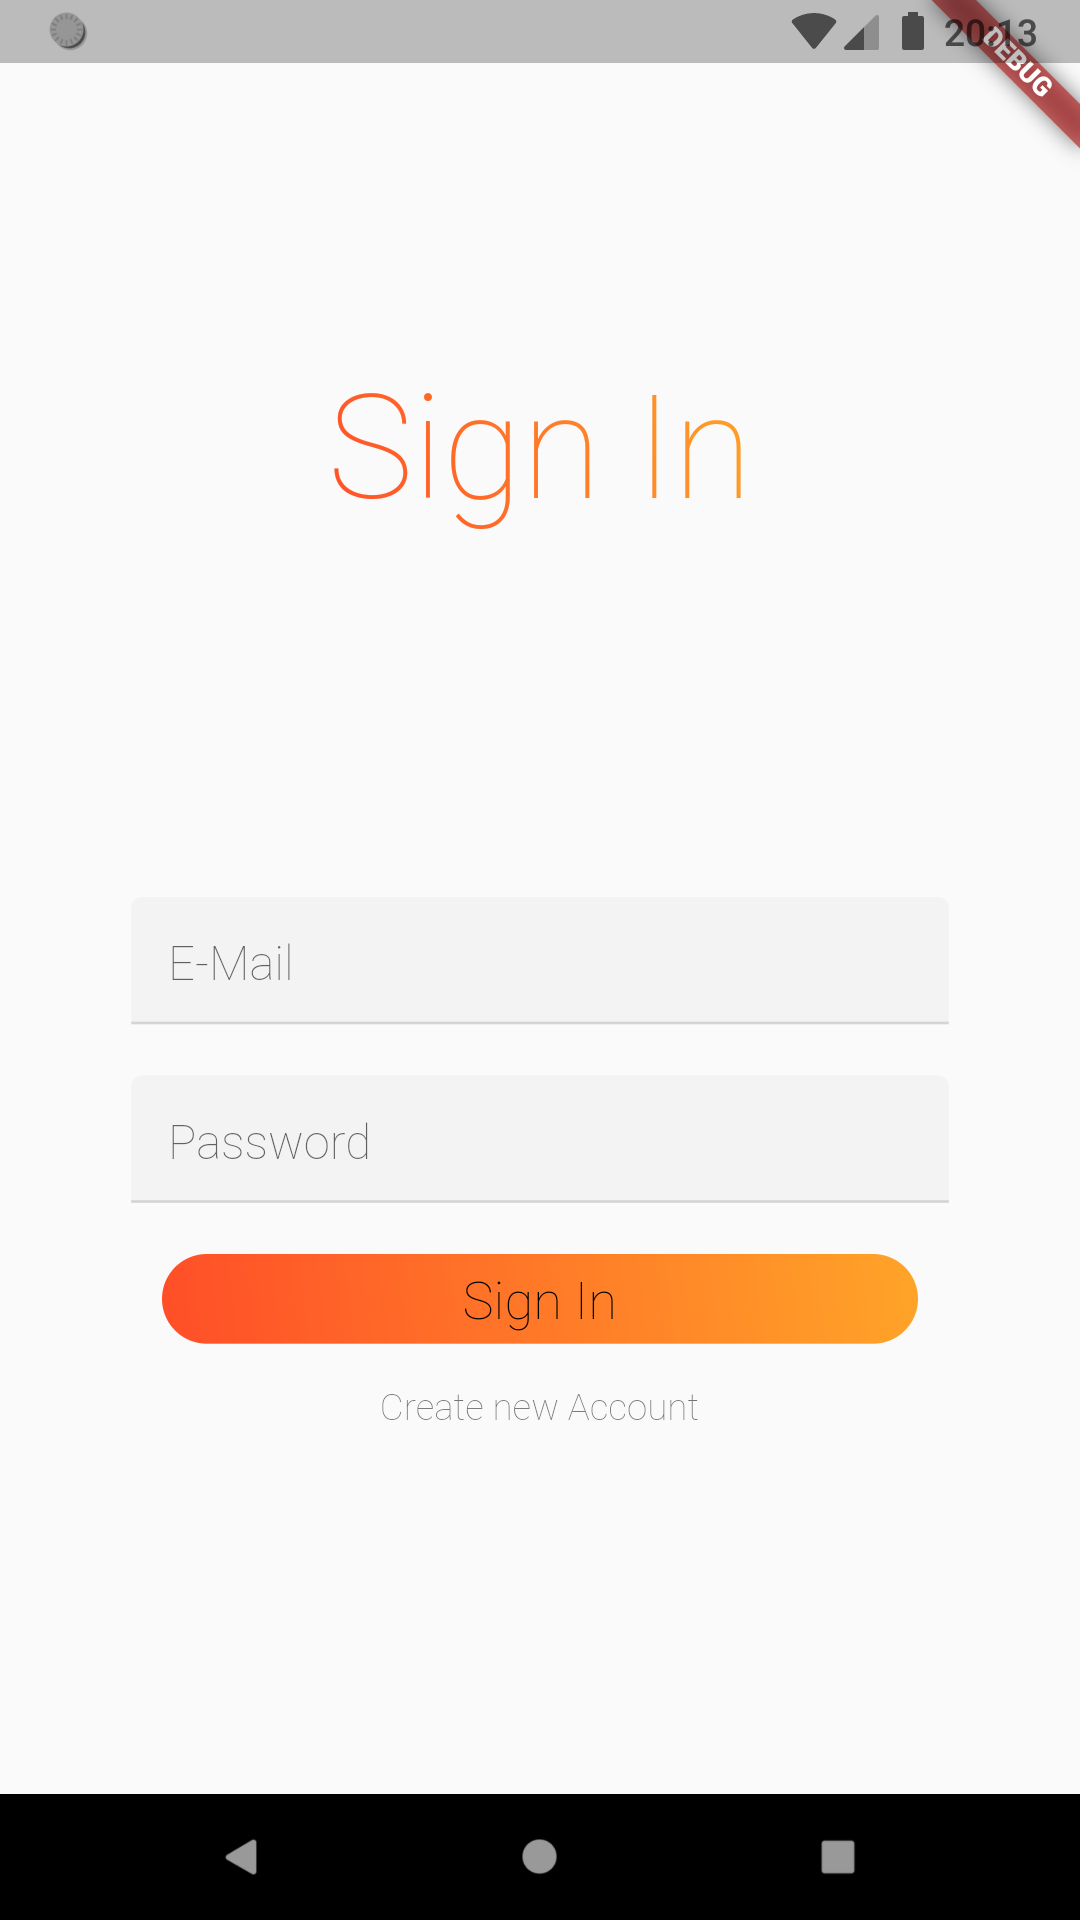
\includegraphics[scale=0.13]{Benutzeroberfläche/images/screenshot_login_1.png}
	\caption{}
	\label{fig:login_a}
	\end{subfigure}
	\begin{subfigure}{0.33\textwidth}
	\centering
	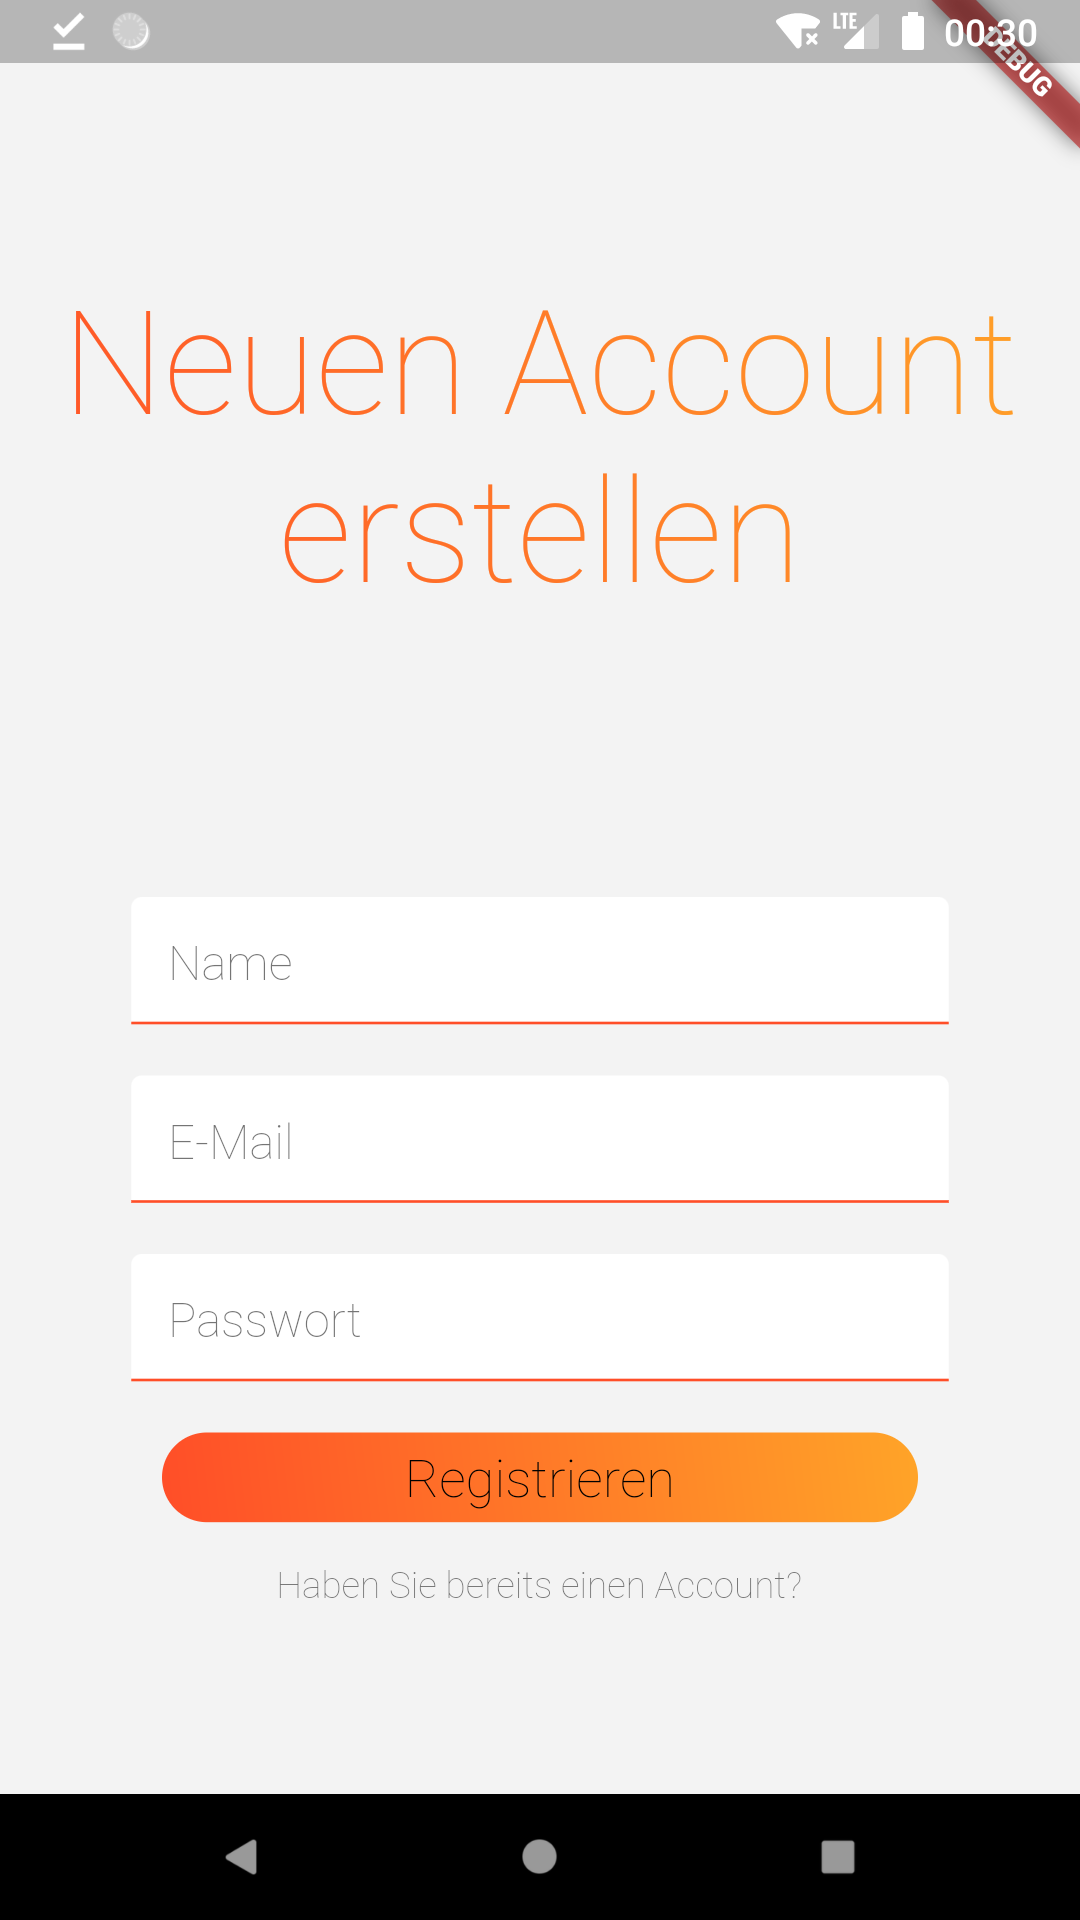
\includegraphics[scale=0.13]{Benutzeroberfläche/images/screenshot_login_2.png}
	\caption{}
	\label{fig:login_b}
	\end{subfigure}
	\begin{subfigure}{0.33\textwidth}
	\centering
	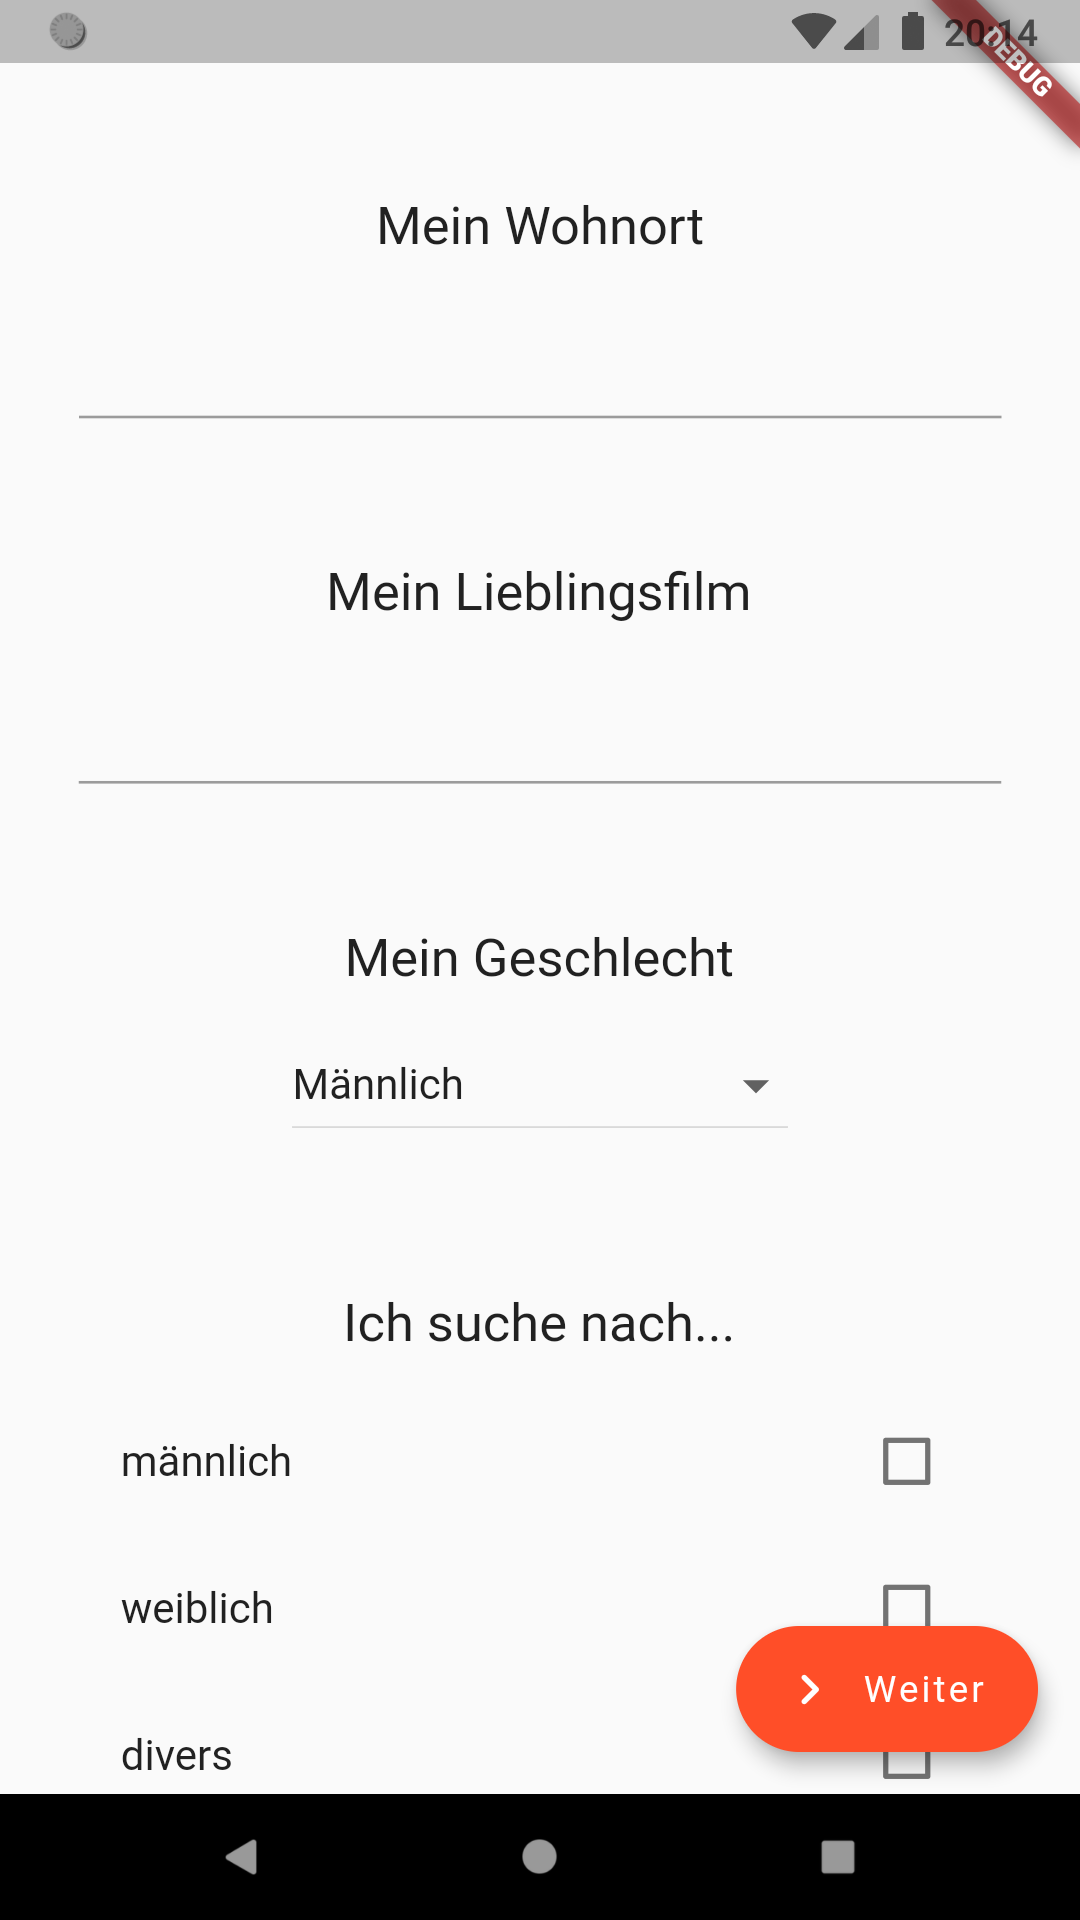
\includegraphics[scale=0.13]{Benutzeroberfläche/images/screenshot_login_3.png}
	\caption{}
	\label{fig:login_c}
	\end{subfigure}\\ \vspace{1cm}	
	
	\begin{subfigure}{0.33\textwidth}
	\centering
	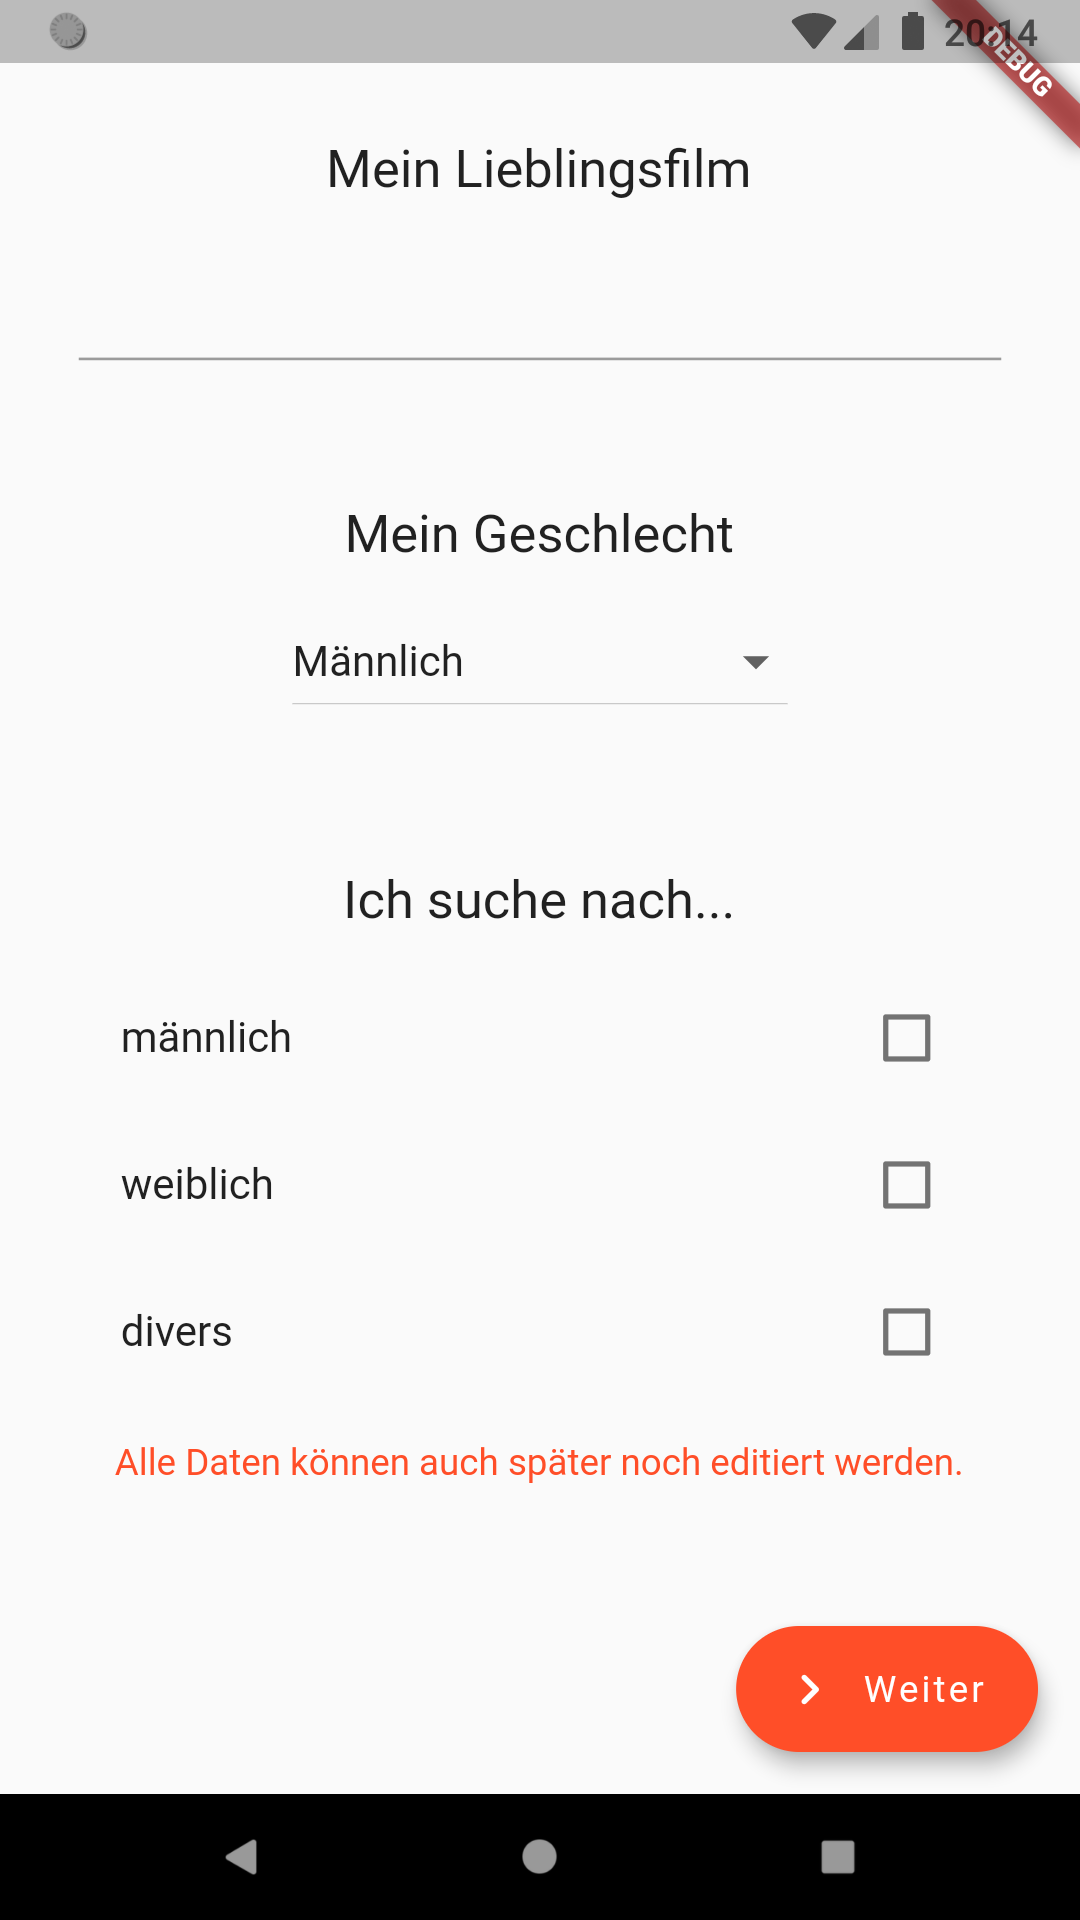
\includegraphics[scale=0.13]{Benutzeroberfläche/images/screenshot_login_4.png}
	\caption{}
	\label{fig:login_d}
	\end{subfigure}
	\begin{subfigure}{0.33\textwidth}
	\centering
	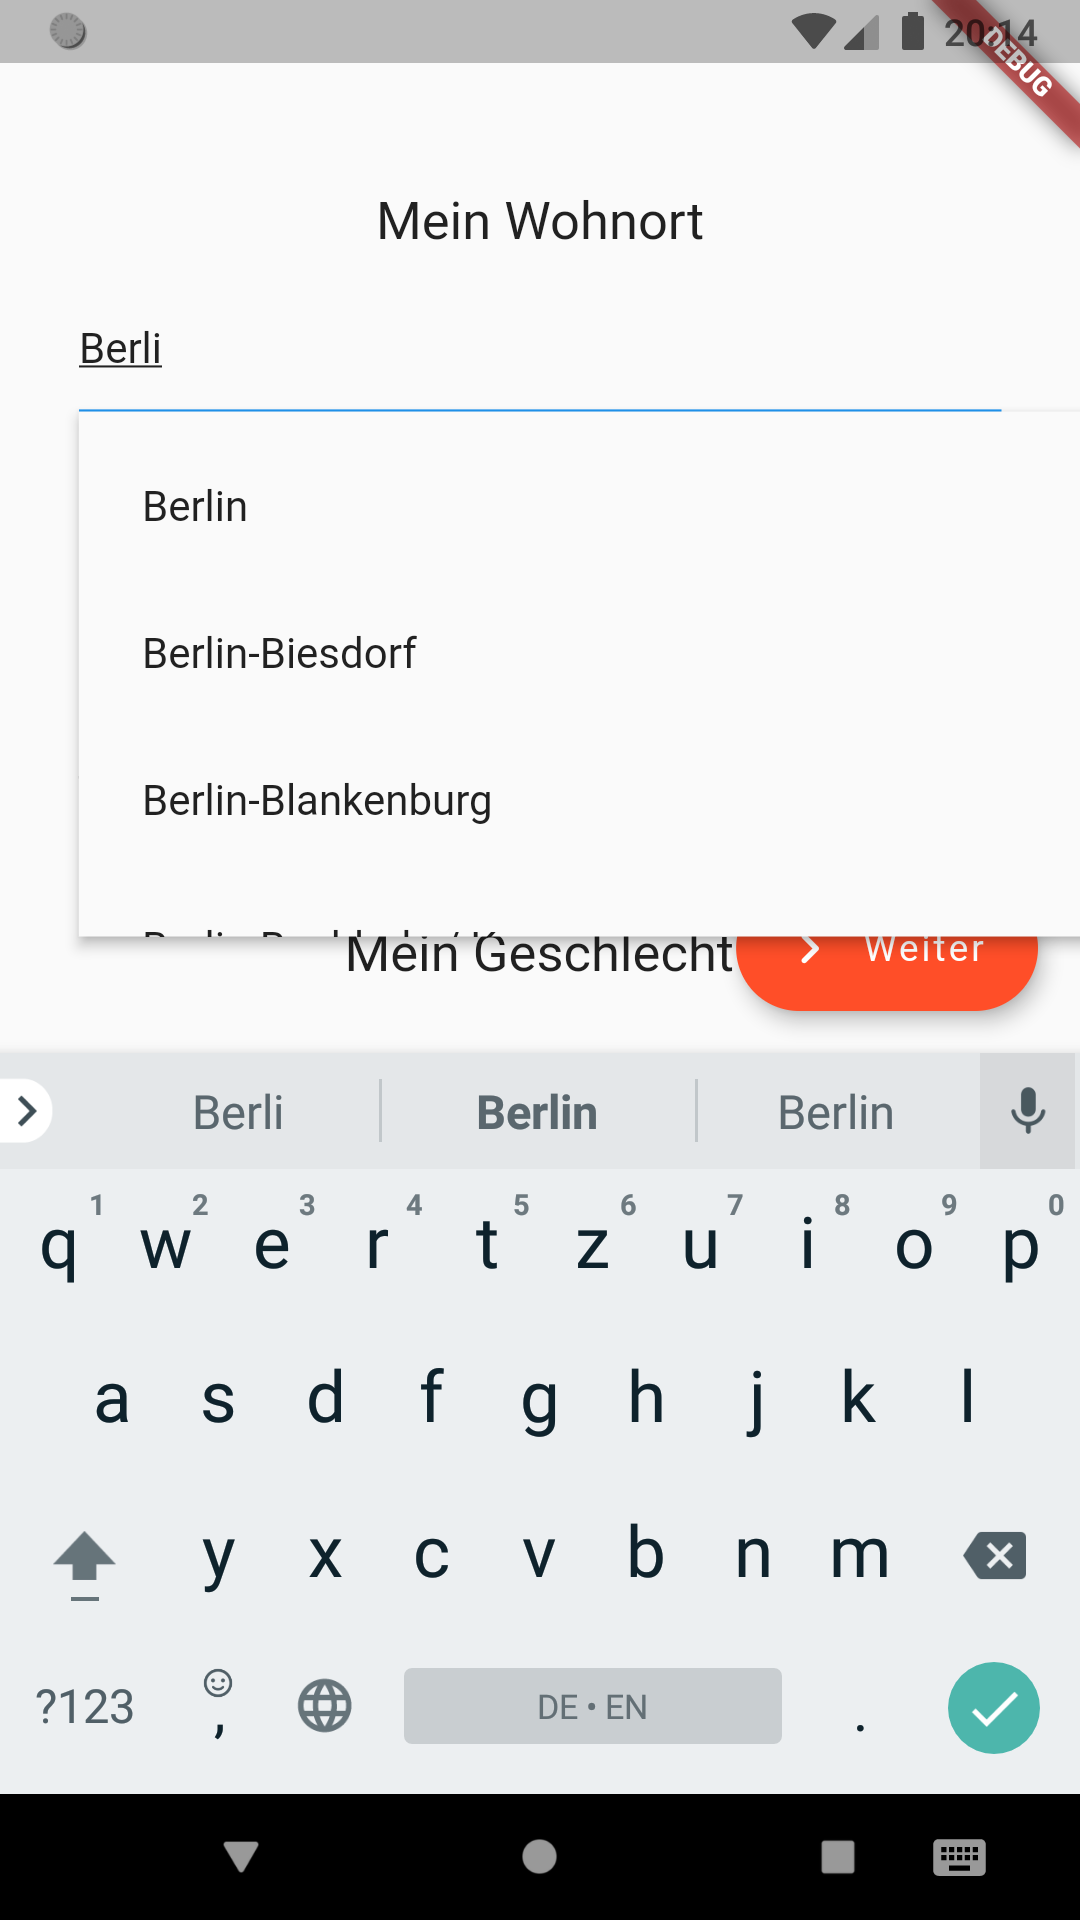
\includegraphics[scale=0.13]{Benutzeroberfläche/images/screenshot_login_5.png}
	\caption{}
	\label{fig:login_e}
	\end{subfigure}
	\begin{subfigure}{0.33\textwidth}
	\centering
	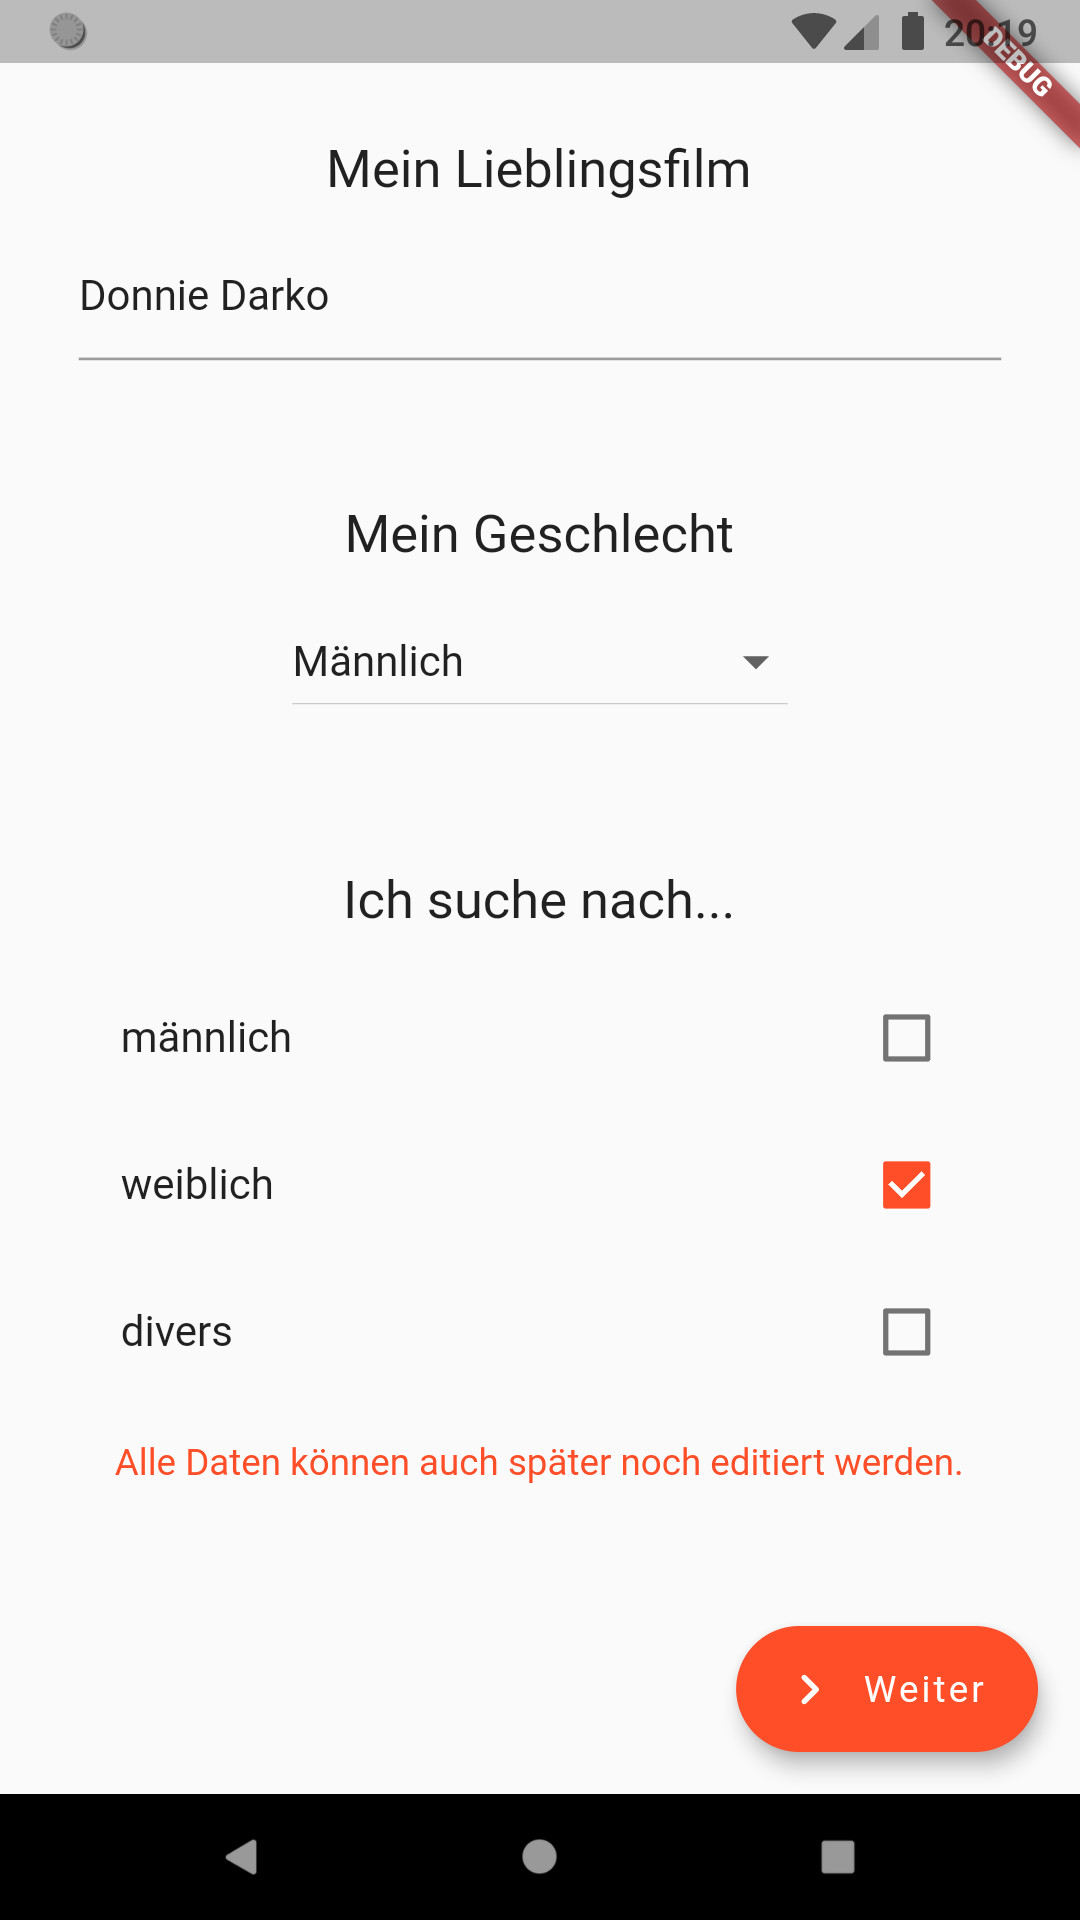
\includegraphics[scale=0.13]{Benutzeroberfläche/images/screenshot_login_6.png}
	\caption{}
	\label{fig:login_f}
	\end{subfigure}
\caption{Der Login-Screen von StreamSwipe und alle damit zusammenhängenden Seiten. Man sieht (a) das Einloggen bei bestehendem Account, (b) das Erstellen eines Accounts, (c) und (d) das Formular für die weiter benötigten Profildaten, (e) Ein Texteingabefeld mit Autovervollständigung als Dropdownmenü und (f) eine ausgefüllte Formular.}
\label{fig:login_alle}
\end{figure}
\clearpage



\subsubsection{Home-Screen}
\label{sec:homescreen}

Da davon ausgegangen wird, dass der User sich nicht nach jeder Nutzung ab- und wieder anmeldet, erscheint im alltäglichen Gebrauch der in Abbildung \ref{fig:homescreen_alle} dargestellte Bildschirm zuerst. Demnach bietet es sich an Ereignisse wie neue Matches und neue Nachrichten hier anzuzeigen. Diese werden wie Abbildungen \ref{fig:homescreen_a} und \ref{fig:homescreen_b} zeigen klar strukturiert in Abschnitte eingegliedert, welche mit Überschriften kenntlich gemacht sind. Die einzelnen Matches befinden sich mit allen dazugehörenden Funktionen und Informationen jeweils auf einer Karte. Durch diese Karten kann mit einer von anderen \mbox{Apps} bekannten horizontalen Swipemechanik navigiert werden. Weiterführende Funktionen wie das Starten eines Chats oder das Löschen des Matches werden durch  Antippen von allgemein verständlichen Icons ausgeführt. \\
Auch auf diesem Screen findet sich einerseits das bereits eingeführte Farbschema wieder und es werden andererseits ebenfalls Semantiken verwendet. Bei den neuen Nachrichten wird jeweils der Benutzername vorgelesen und bei den neuen Matches je nach ausgewähltem Bereich der Filmname, die Icons oder der Text dazwischen.\\
Am unteren Bildschirmrand ist eine sogenannte Bottom-Navigation-Bar zu sehen. Sie ermöglicht eine kompakte und anschauliche Navigation durch die relevanten Bildschirme. Außerdem zeigt sie an welcher Bildschirm aktuell ausgewählt ist. Liest der Screenreader die Semantik hiervon, gibt er die Bezeichnung des aktuellen Bildschirms sowie die Anzahl der weiteren Möglichkeiten an. \\
%TODO Motorische Herausforderungen!!! Anklicken des Filmposters aktiviert auch Chat?

\begin{figure}[tbt]
	\begin{subfigure}{0.33\textwidth}
	\centering
	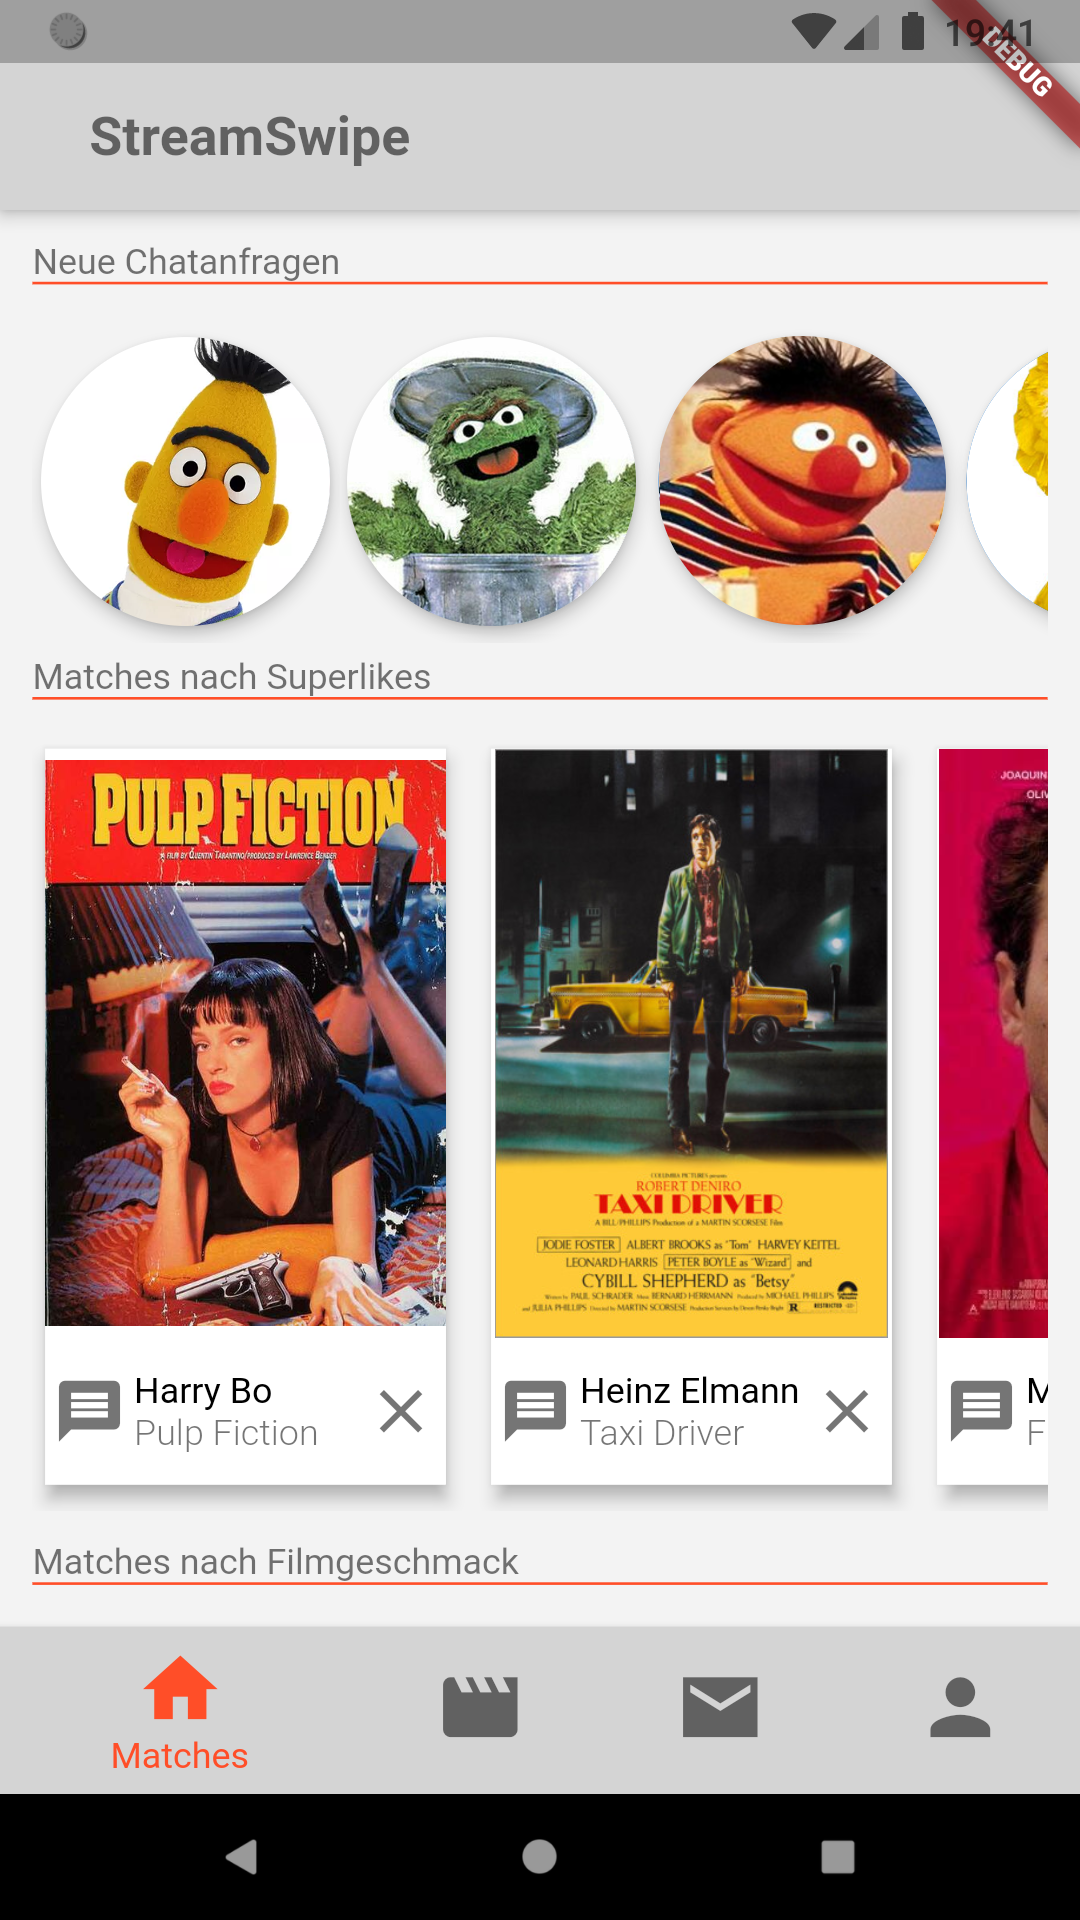
\includegraphics[scale=0.13]{Benutzeroberfläche/images/screenshot_homescreen_1.png}
	\caption{}
	\label{fig:homescreen_a}
	\end{subfigure}
	\begin{subfigure}{0.33\textwidth}
	\centering
	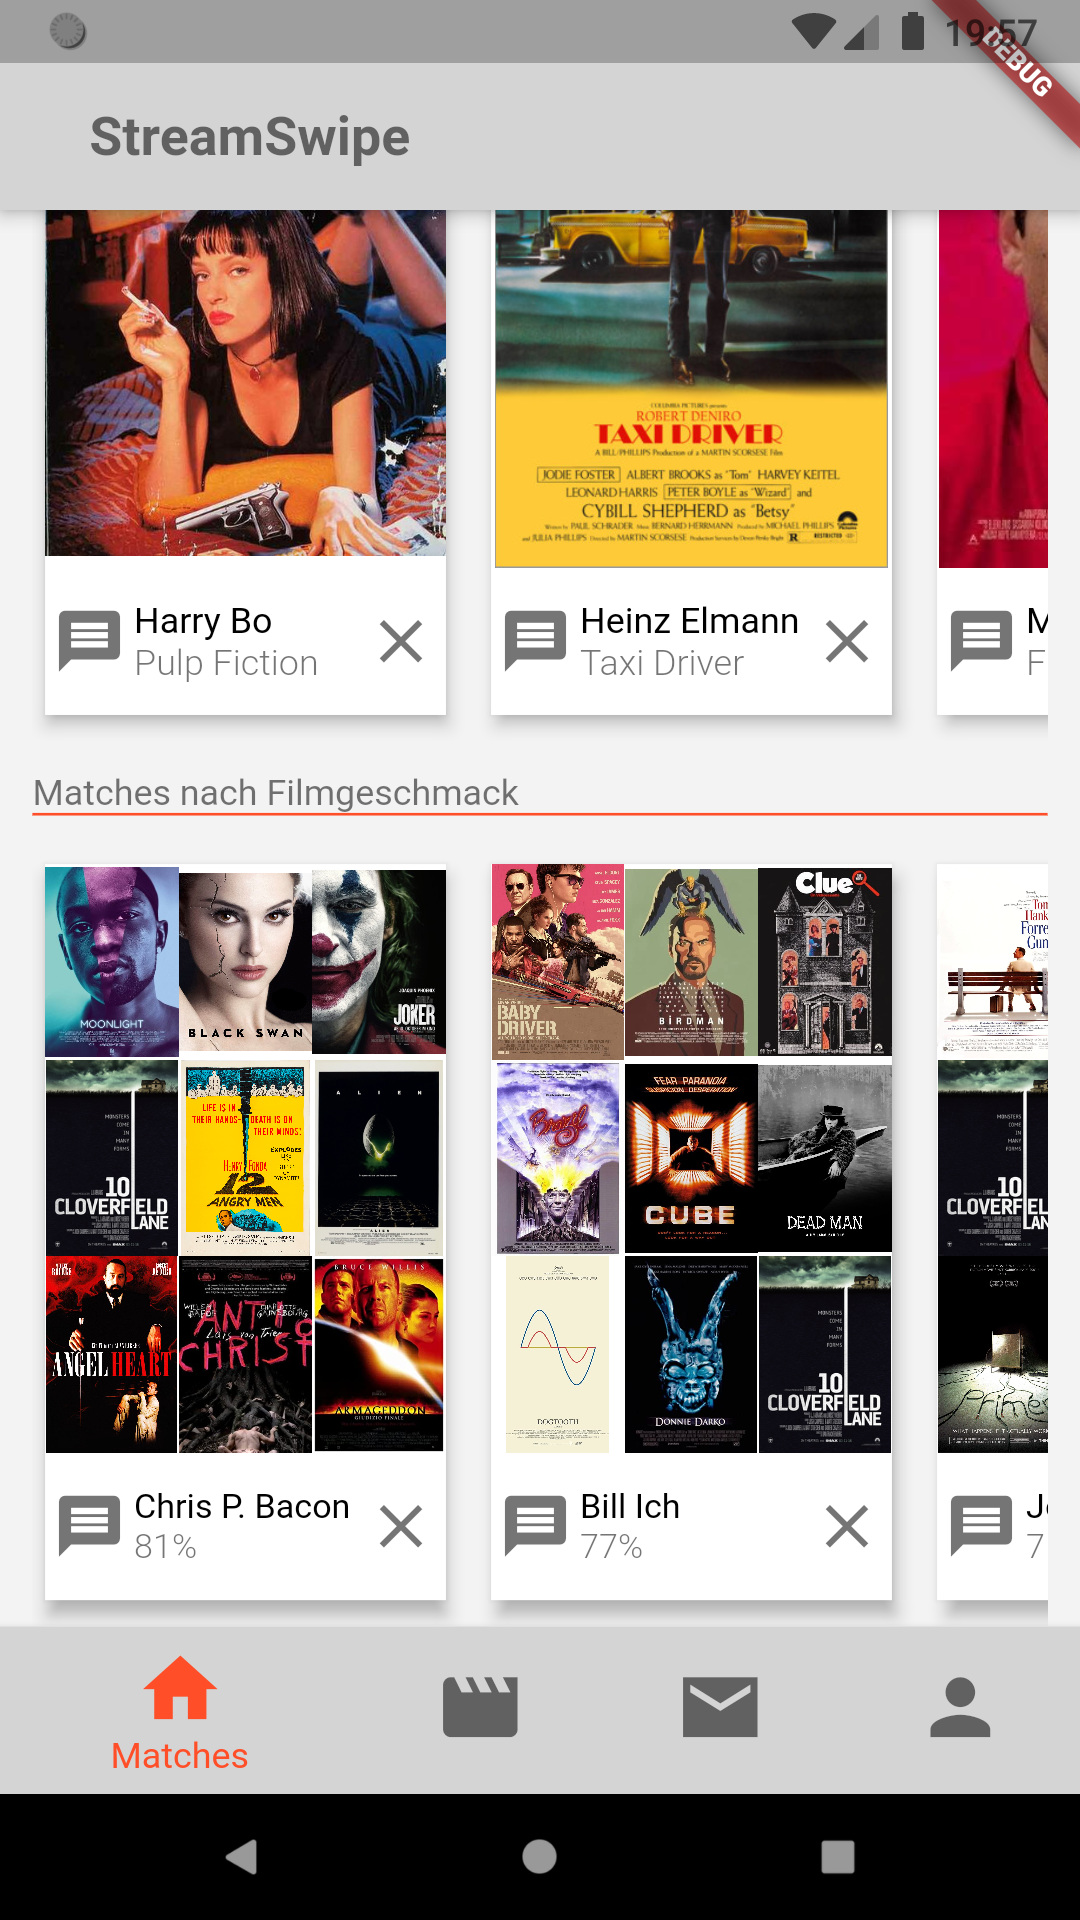
\includegraphics[scale=0.13]{Benutzeroberfläche/images/screenshot_homescreen_2.png}
	\caption{}
	\label{fig:homescreen_b}
	\end{subfigure}
	\begin{subfigure}{0.33\textwidth}
	\centering
	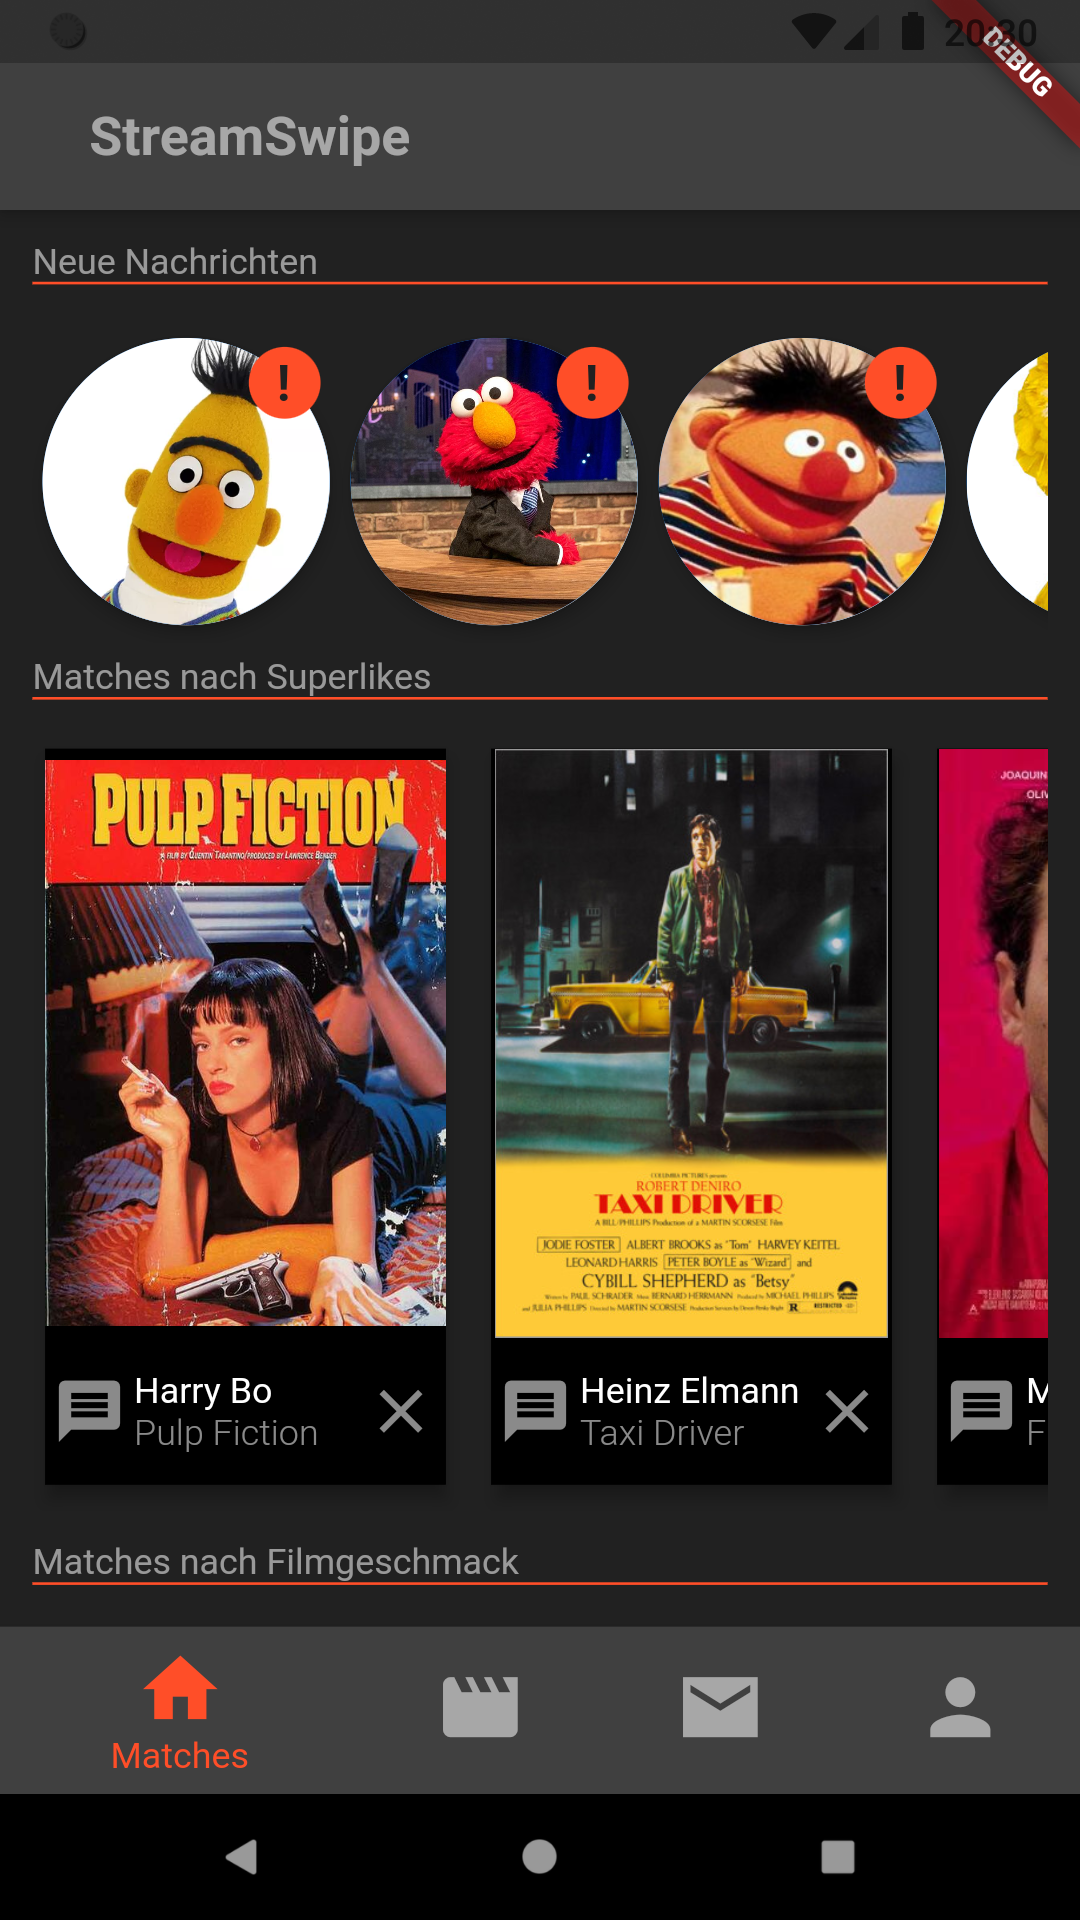
\includegraphics[scale=0.13]{Benutzeroberfläche/images/screenshot_darkmode_1.png}
	\caption{}
	\label{fig:homescreen_c}
	\end{subfigure}
\caption{Der Home-Screen, der beim Öffnen der App zuerst gezeigt wird und Neuigkeiten wie neue Nachrichten und Matches zusammenfasst. Um den gesamten Inhalt dieser Seite sehen zu können, wird in (a) der obere Abschnitt und in (b) der untere Abschnitt gezeigt. Hat der User in den Systemeinstellungen den dunklen Modus aktiviert, so wird (c) der Home-Screen wie alle anderen Screens angepasst.}
\label{fig:homescreen_alle}
\end{figure}




\subsubsection{Swipe-Screen}
\label{sec:swipescreen}
Auf dem Swipe-Screen (Abbildungen \ref{fig:swipescreen_alle}) findet die Bewertung der Filme statt. Durch das hier verwendete Matchingsystem mithilfe des Filmgeschmacks unterscheidet sich StreamSwipe von anderen Apps und erhält so einen innovativen, individuellen Charakter, womit diese Seite das Herzstück der App bildet.\\
Das zuvor eingeführte Farbschema bleibt auch hier erhalten, wie Abbildung \ref{fig:swipescreen_a} zeigt. Eine Überschrift im selben Stil wie bereits aus Abschnitt \ref{sec:homescreen} bekannt, verdeutlicht durch eine Frage nach welcher Motivation die Filmauswahl getroffen werden soll. Zentral im Bild ist eine Liste von Postern der zu beurteilenden Filme. Wie bereits durch die Datingapp Tinder verbreitet, werden die vier Antwortmöglichkeiten durch eine Swipe-Bewegung in eine der vier Richtungen ausgewählt. Abhängig von der Position des Fingers auf dem Touchscreen bewegt sich das Filmposter innerhalb des Bildschirms, was den Effekt einer frei beweglichen Karte hervorruft. Um klarzustellen welche Swipe-Richtung für welche Entscheidung steht, verfärbt sich der jeweilige Indikator in der unteren Reihe bei Verschiebung des Filmposter. Beide diese Animationen sind in Abbildung \ref{fig:swipescreen_d} zu sehen. Die Indikatoren sind mit Icons versehen, zeigen aber durch Drücken welche Entscheidung sie repräsentieren und in welche Richtung der User dafür swipen muss, wie Abbildung \ref{fig:swipescreen_c} am Beispiel des rechten Indikators zeigt. \\
Durch Antippen des Filmposters werden weitere Informationen zu dem jeweiligen Film dargestellt, wie in Abbildung \ref{fig:swipescreen_b} zu sehen. Gleichfalls wird durch ein einfaches Antippen wieder zurück  zu den Postern gewechselt. Eine Rotations-Animation verdeutlicht die Illusion der Karten.\\
Alle diese für die Bedienung der App grundlegenden Steuerungen verlangen keine feinmotorischen Eingaben und können problemlos von Personen mit motorischen Einschränkungen genutzt werden. Auch dieser Bildschirm ist vollkommen mit Semantiken ausgestattet. Anstelle des Filmposters wird der Name des Films ausgelesen und für die vier Indikatoren am unteren Rand werden jeweils deren Funktion und durch welche Swipe-Richtung sie erreicht werden vorgelesen. Sämtliche Textfelder können ebenfalls problemlos von einem Screenreader gelesen werden.



\begin{figure}[tbt]
	\begin{subfigure}{0.33\textwidth}
	\centering
	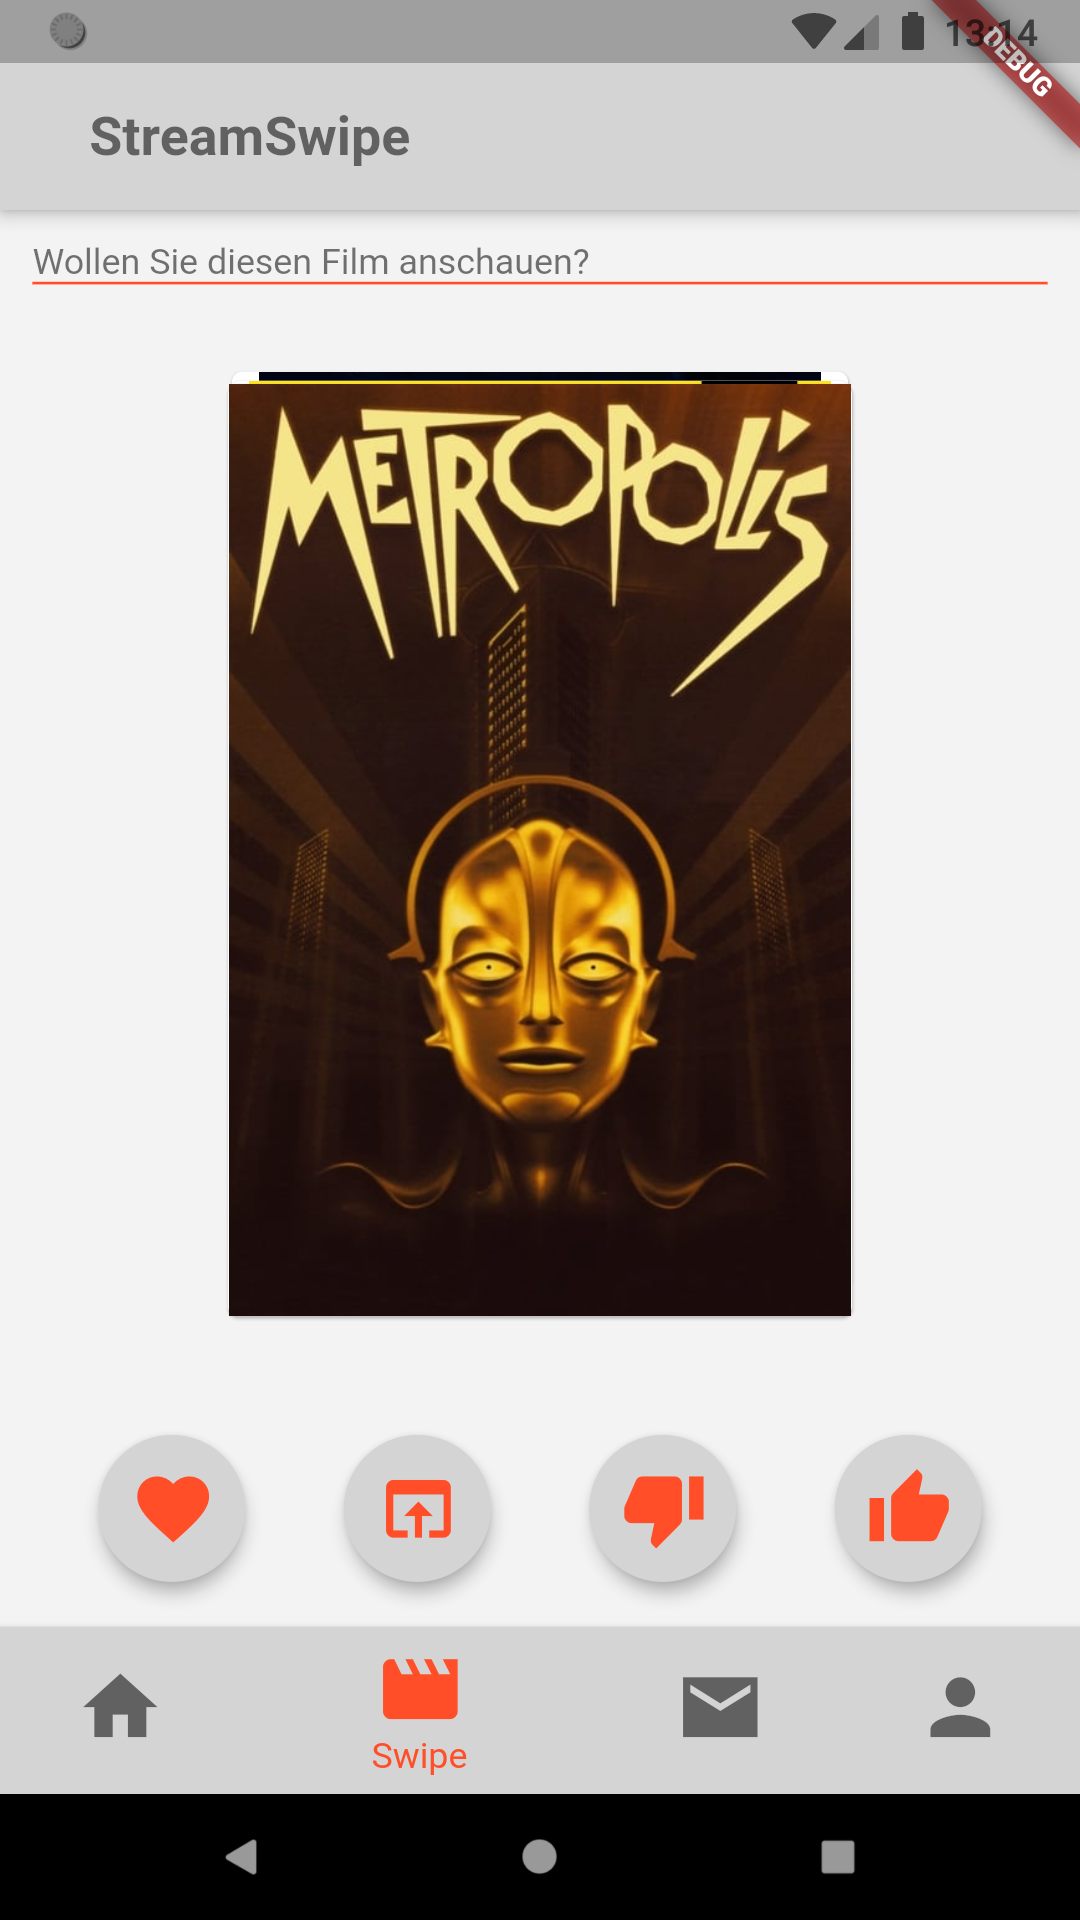
\includegraphics[scale=0.13]{Benutzeroberfläche/images/screenshot_swipescreen1.png}
	\caption{}
	\label{fig:swipescreen_a}
	\end{subfigure}
	\begin{subfigure}{0.33\textwidth}
	\centering
	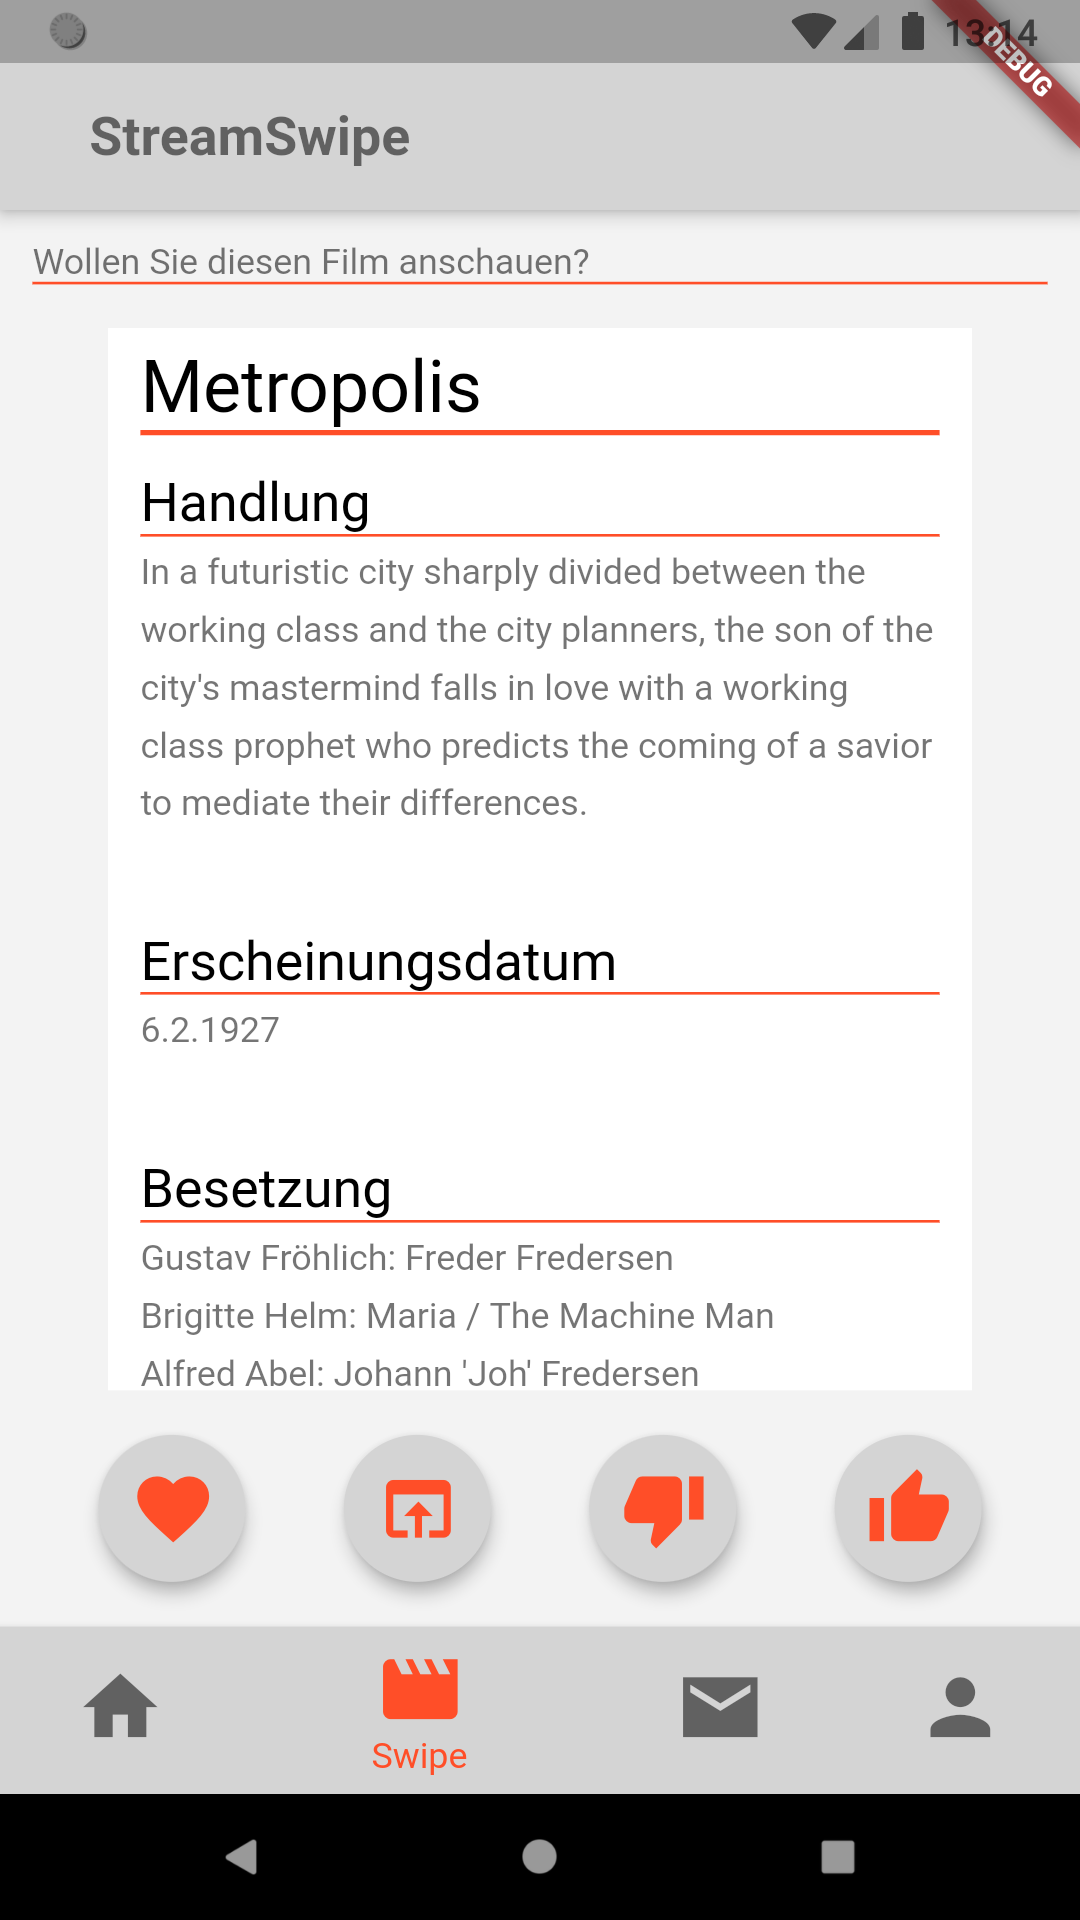
\includegraphics[scale=0.13]{Benutzeroberfläche/images/screenshot_swipescreen2.png}
	\caption{}
	\label{fig:swipescreen_b}
	\end{subfigure}
	\begin{subfigure}{0.33\textwidth}
	\centering
	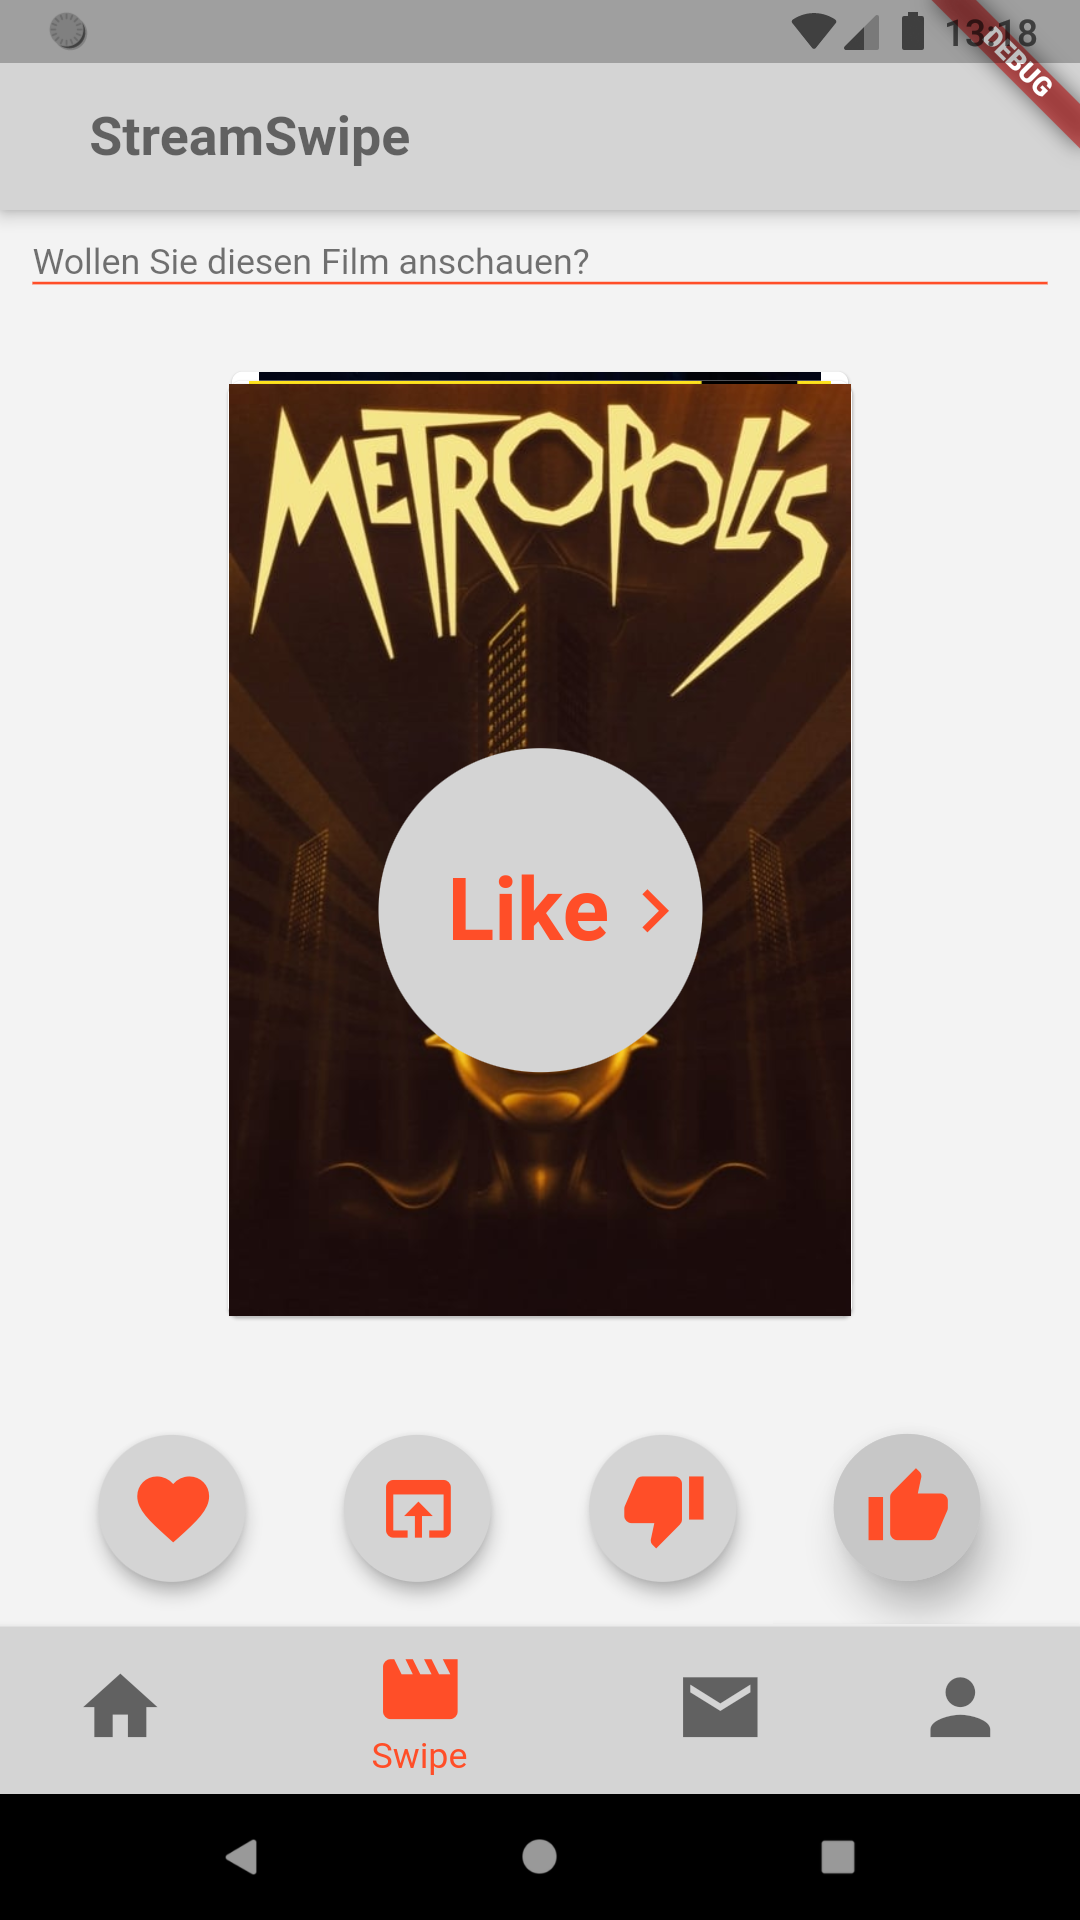
\includegraphics[scale=0.1742]{Benutzeroberfläche/images/screenshot_swipescreen3.png}
	\caption{}
	\label{fig:swipescreen_c}
	\end{subfigure}\\ \vspace{1cm}	
	
	\begin{subfigure}{0.33\textwidth}
	\centering
	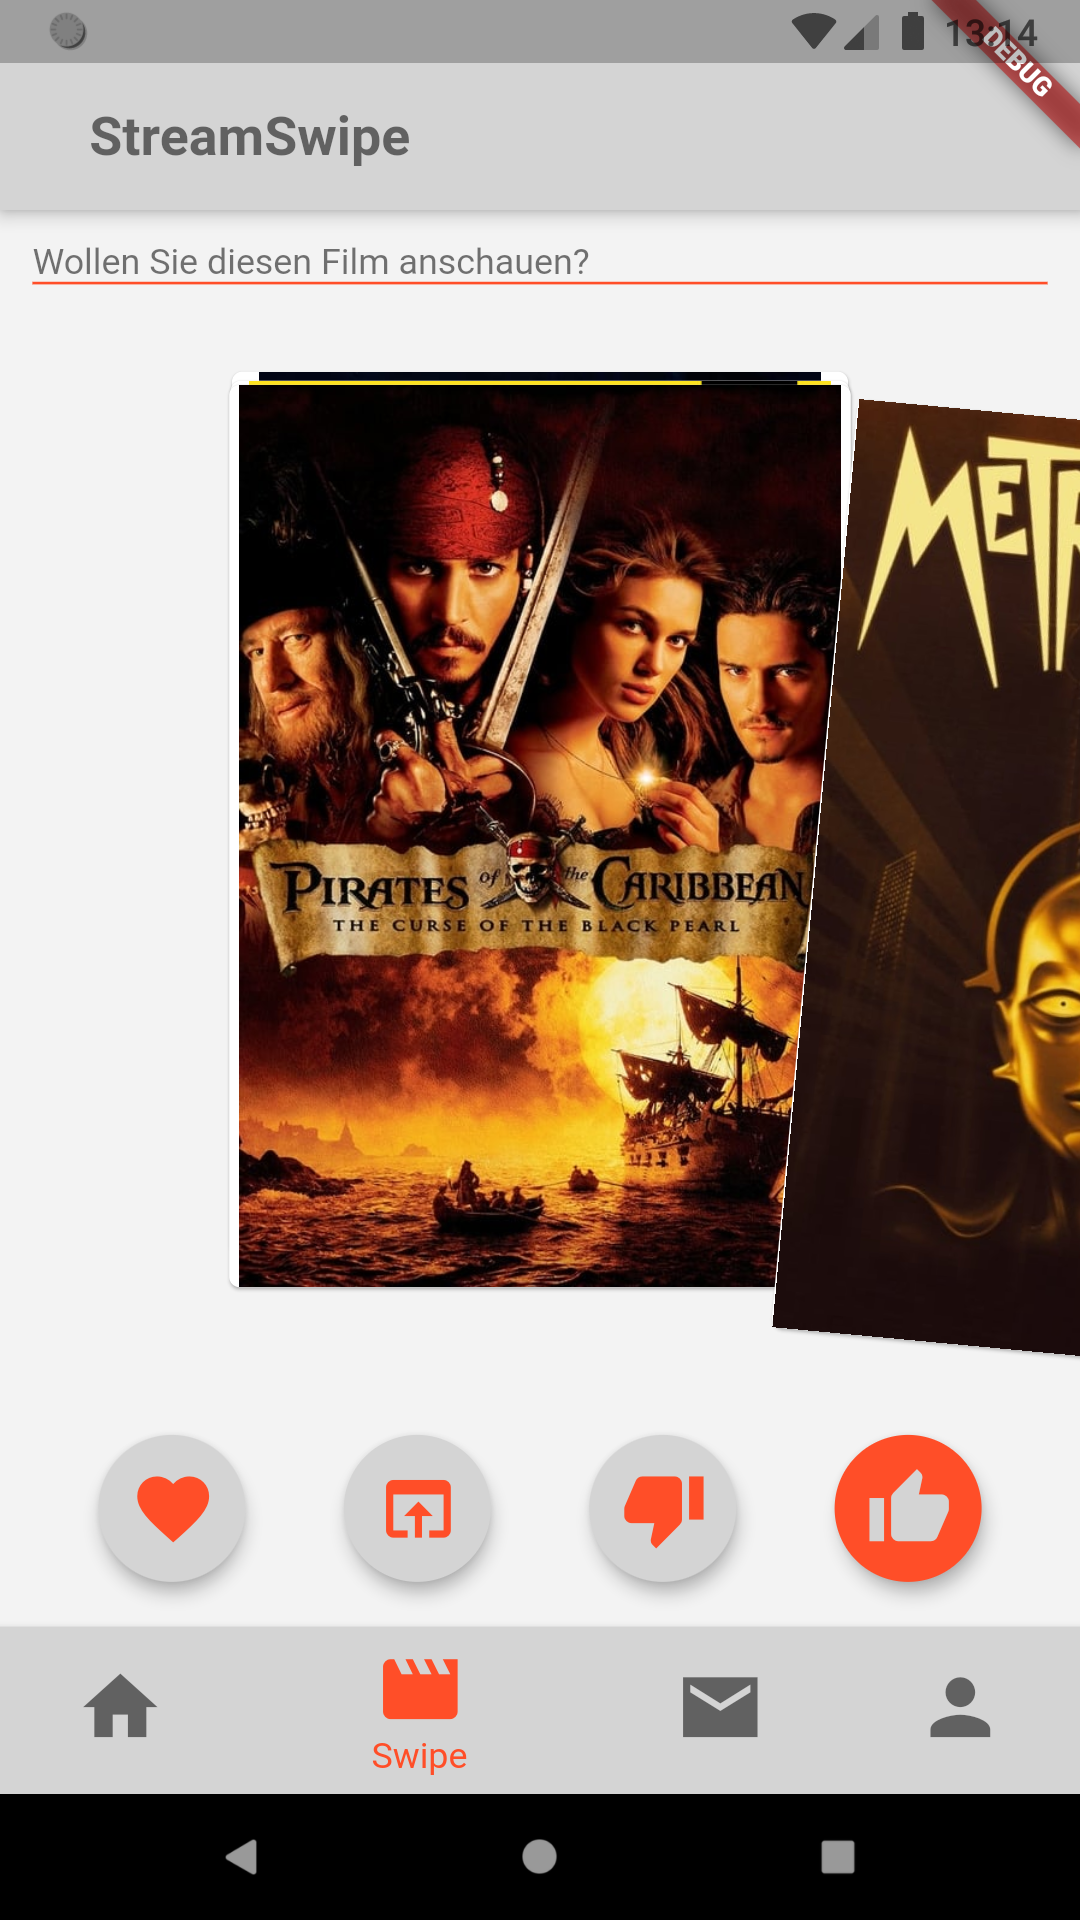
\includegraphics[scale=0.13]{Benutzeroberfläche/images/screenshot_swipescreen4.png}
	\caption{}
	\label{fig:swipescreen_d}
	\end{subfigure}
	\begin{subfigure}{0.33\textwidth}
	\centering
	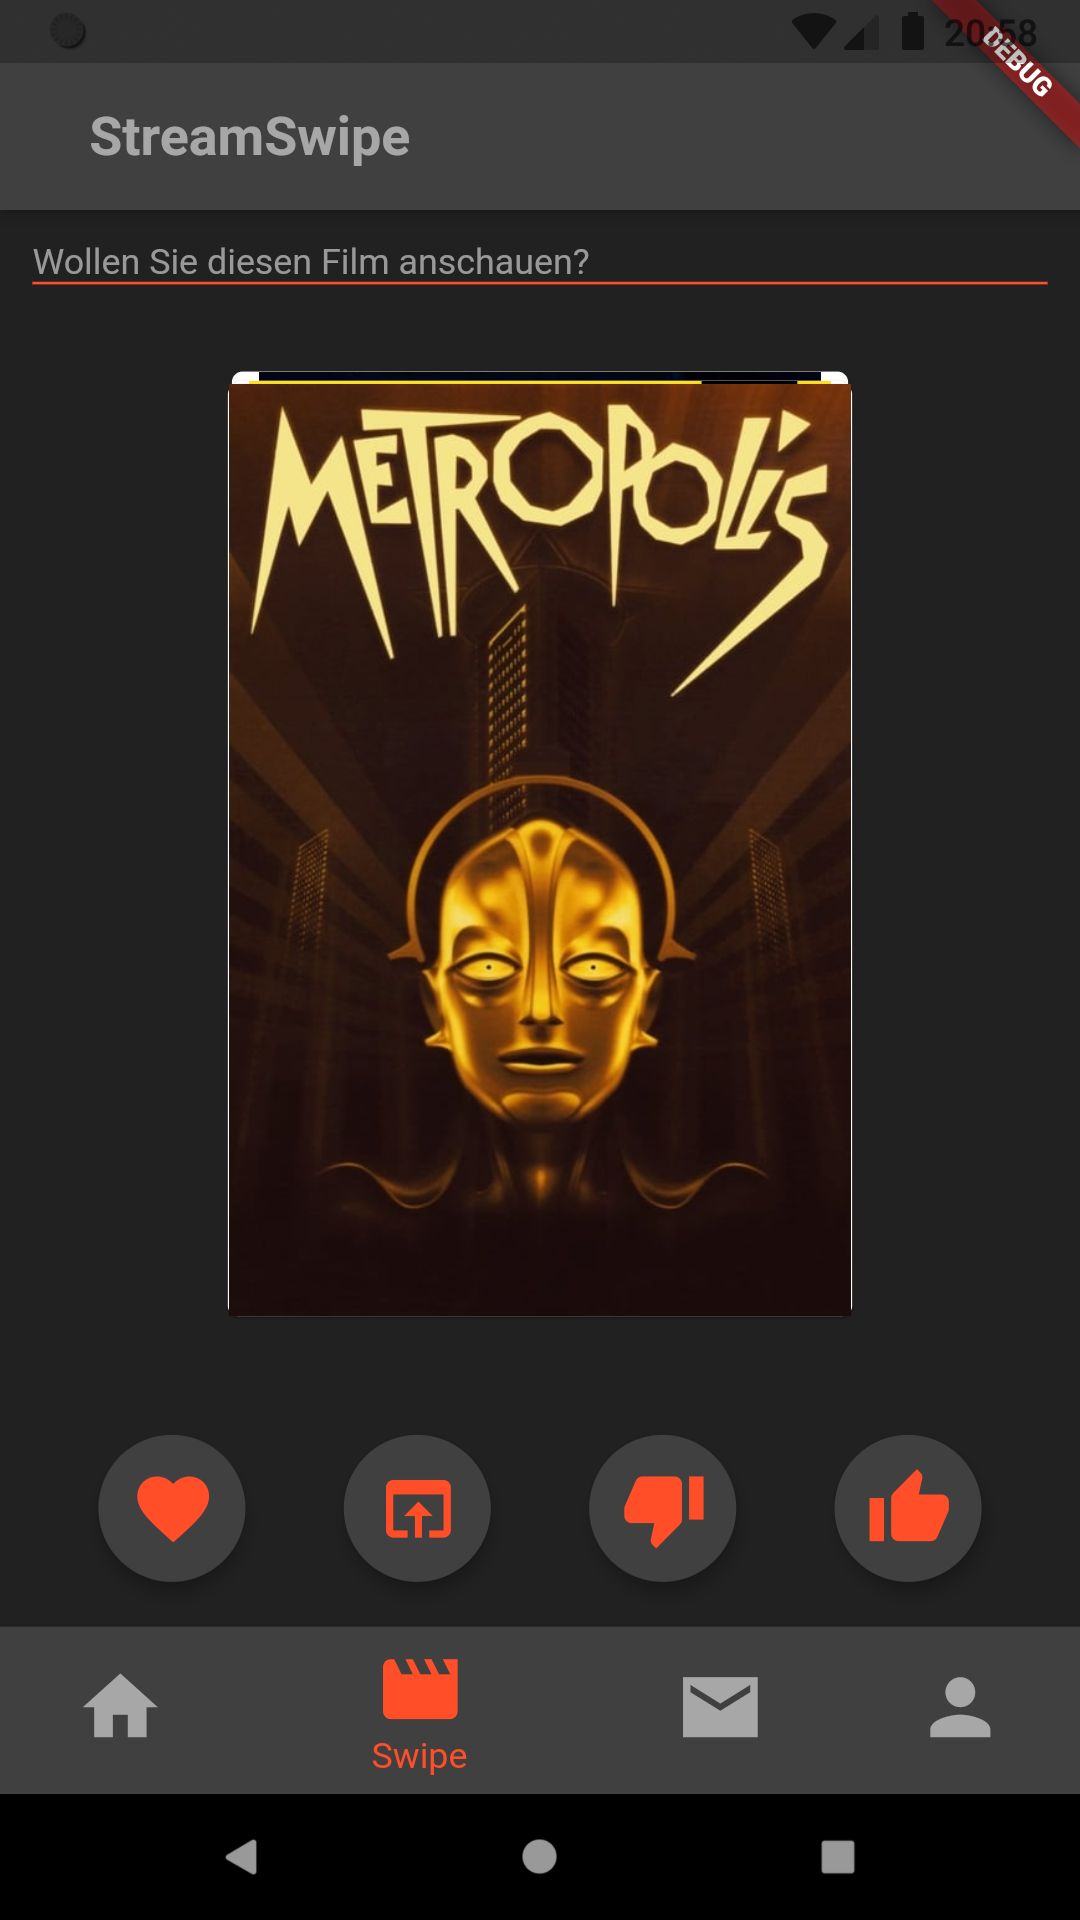
\includegraphics[scale=0.13]{Benutzeroberfläche/images/screenshot_darkmode_2.png}
	\caption{}
	\label{fig:swipescreen_e}
	\end{subfigure}
\caption{Darstellungen und Funktionen des Swipe-Screens mit (a) der Standarddarstellung, (b) weiteren Filminformationen, (c) einer Animation beim Drücken einer der Indikatoren und (d) der Swipe-Animation.  Hat der User in den Systemeinstellungen den dunklen Modus aktiviert, so wird (e) der Swipe-Screen wie alle anderen Screens angepasst.}
\label{fig:swipescreen_alle}
\end{figure}
\clearpage


\subsubsection{Chat}
\label{sec:UI-Chat}
Die Chatseite ist in eine Liste aus aktiven Chats und eine Warteliste aufgeteilt, siehe \ref{fig:chat_a} und \ref{fig:chat_b}. Um zwischen diesen beiden Listen zu wechseln werden Tabs eingesetzt, wie sie aus Windowsanwendungen bekannt sind. Zwischen diesen Tabs kann entweder gewechselt werden, indem ein anderes Tabfenster angetippt wird, oder der gesamte Bildschirm mit einer Geste zur Seite gewischt wird. Bei jedem Element der Chatliste ist der jeweilige Benutzername und die neueste Nachricht zu sehen, dazu wird falls vorhanden entweder ein Profilbild oder eine einfarbige Fläche mit dem Anfangsbuchstaben des Namens angezeigt. Chat Requests können jeweils durch das Schieben nach links angenommen oder nach rechts ablehnt werden, wie in den Abbildungen \ref{fig:chat_c}, bzw. \ref{fig:chat_d} zu sehen ist. Diese Mechanik wird häufig in Email-Apps zum Löschen oder Verschieben der Mails benutzt.\\ %TODO (screenshots normal, annehmen und ablehnen)
Durch Antippen eines Matches, öffnet sich der Chatverlauf, welcher in Abbildung \ref{fig:chat_e} zu sehen ist. Die Anordnung der Nachrichten innerhalb des Chatverlaufs ist wie aus anderen Messenger bereits bekannt, aber in den Stilfarben von StreamSwipe. Am oberen Bildschirmrand wird der Profilname des Matches angezeigt und rechts davon befindet sich der Button zu dessen Profilseite, auf der genauere Details über diese Person zu finden sind. Die Profilseiten werden in Kapitel \ref{sec:benutzerprofil} genauer vorgestellt. \\
Dem User wird durch das ihm bereits vorgestellte Design und der ausschließlichen Nutzung von bekannter Mechanik ein vertrautes Umfeld geboten. Wie auf jedem Screen passt sich auch hier das Farbschema automatisch an, falls in den Systemeinstellungen des Smartphones das dunkle Design gewählt wurde, wie beispielsweise in Abbildung \ref{fig:chat_f} dargestellt. Neben der Benutzerfreundlichkeit wird auch die Barrierefreiheit beachtet, indem alle Elemente, die nicht bereits aus einem Text bestehen, mit Semantiken ausgestattet werden. Zusätzlich werden keine feinmotorischen Bewegungen zur Navigation durch die Bildschirme benötigt. Bis auf die Eingabe über die Tastatur kann alles über große Flächen oder Wischmechaniken bedient werden. Im Chatverlauf wir die Standardtastatur des Systems verwendet, mit der der Benutzer bereits vertraut ist. 


\begin{figure}[H]
	\begin{subfigure}{0.33\textwidth}
	\centering
	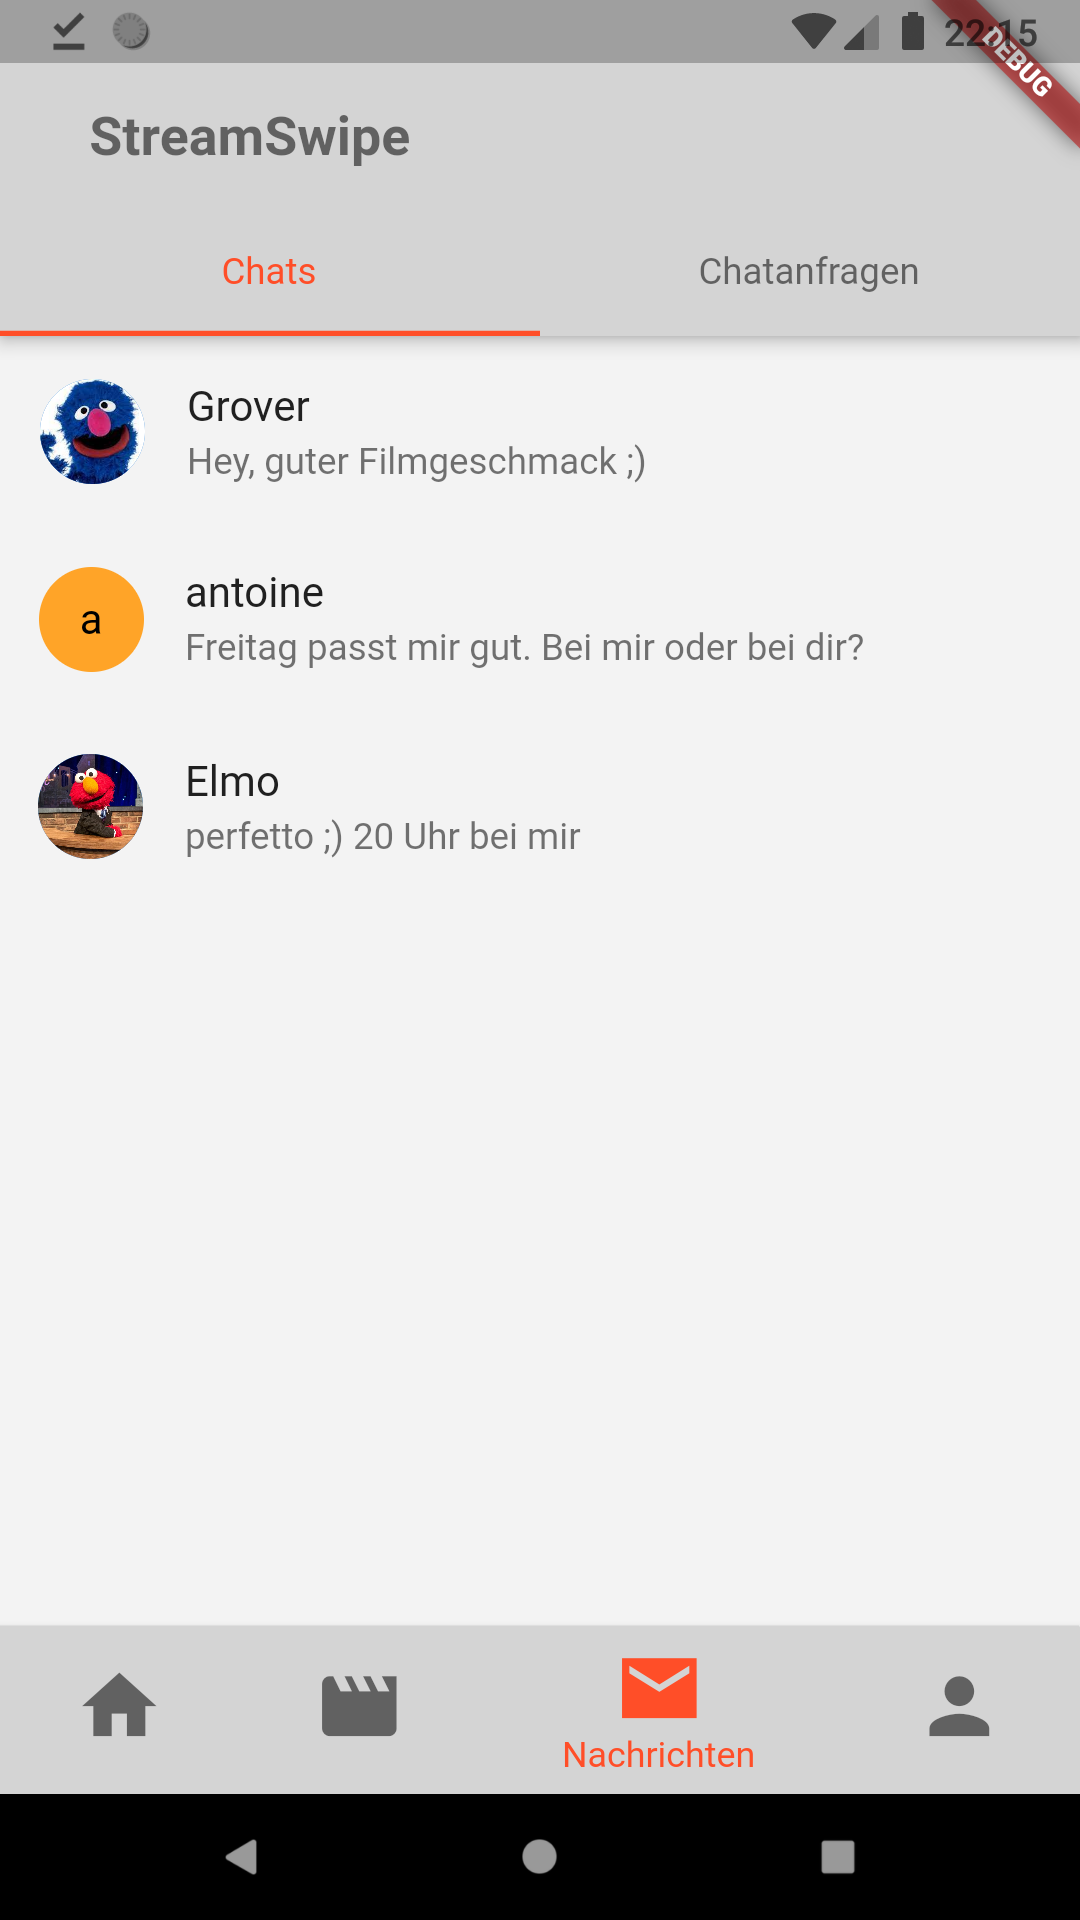
\includegraphics[scale=0.1742]{Benutzeroberfläche/images/screenshot_chat_1.png}
	\caption{}
	\label{fig:chat_a}
	\end{subfigure}
	\begin{subfigure}{0.33\textwidth}
	\centering
	
\includegraphics[scale=0.1742]{Benutzeroberfläche/images/screenshot_chat_2.png}
	\caption{}
	\label{fig:chat_b}
	\end{subfigure}
	\begin{subfigure}{0.33\textwidth}
	\centering
	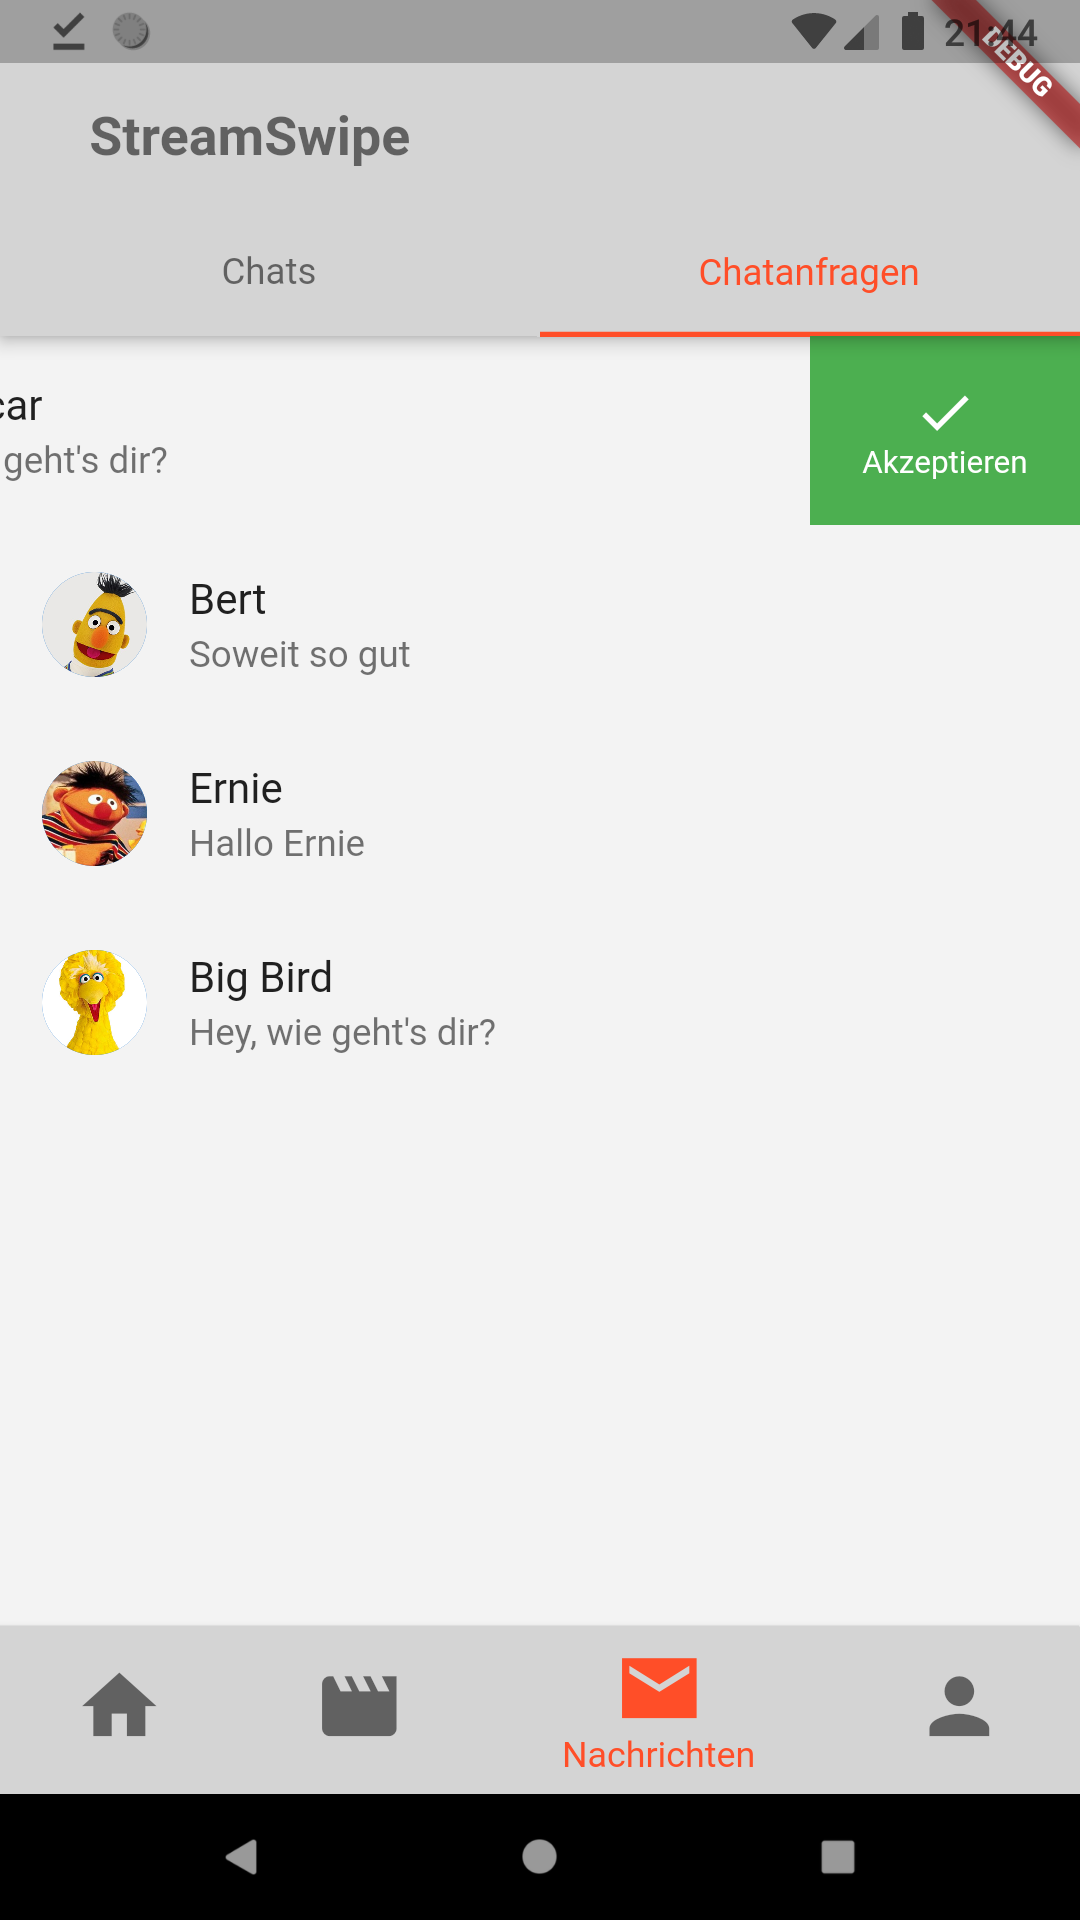
\includegraphics[scale=0.1742]{Benutzeroberfläche/images/screenshot_chat_3.png}
	\caption{}
	\label{fig:chat_c}
	\end{subfigure}\\ \vspace{1cm}	
	
	\begin{subfigure}{0.33\textwidth}
	\centering
	
\includegraphics[scale=0.1741]{Benutzeroberfläche/images/screenshot_chat_4.png}
	\caption{}
	\label{fig:chat_d}
	\end{subfigure}
	\begin{subfigure}{0.33\textwidth}
	\centering
	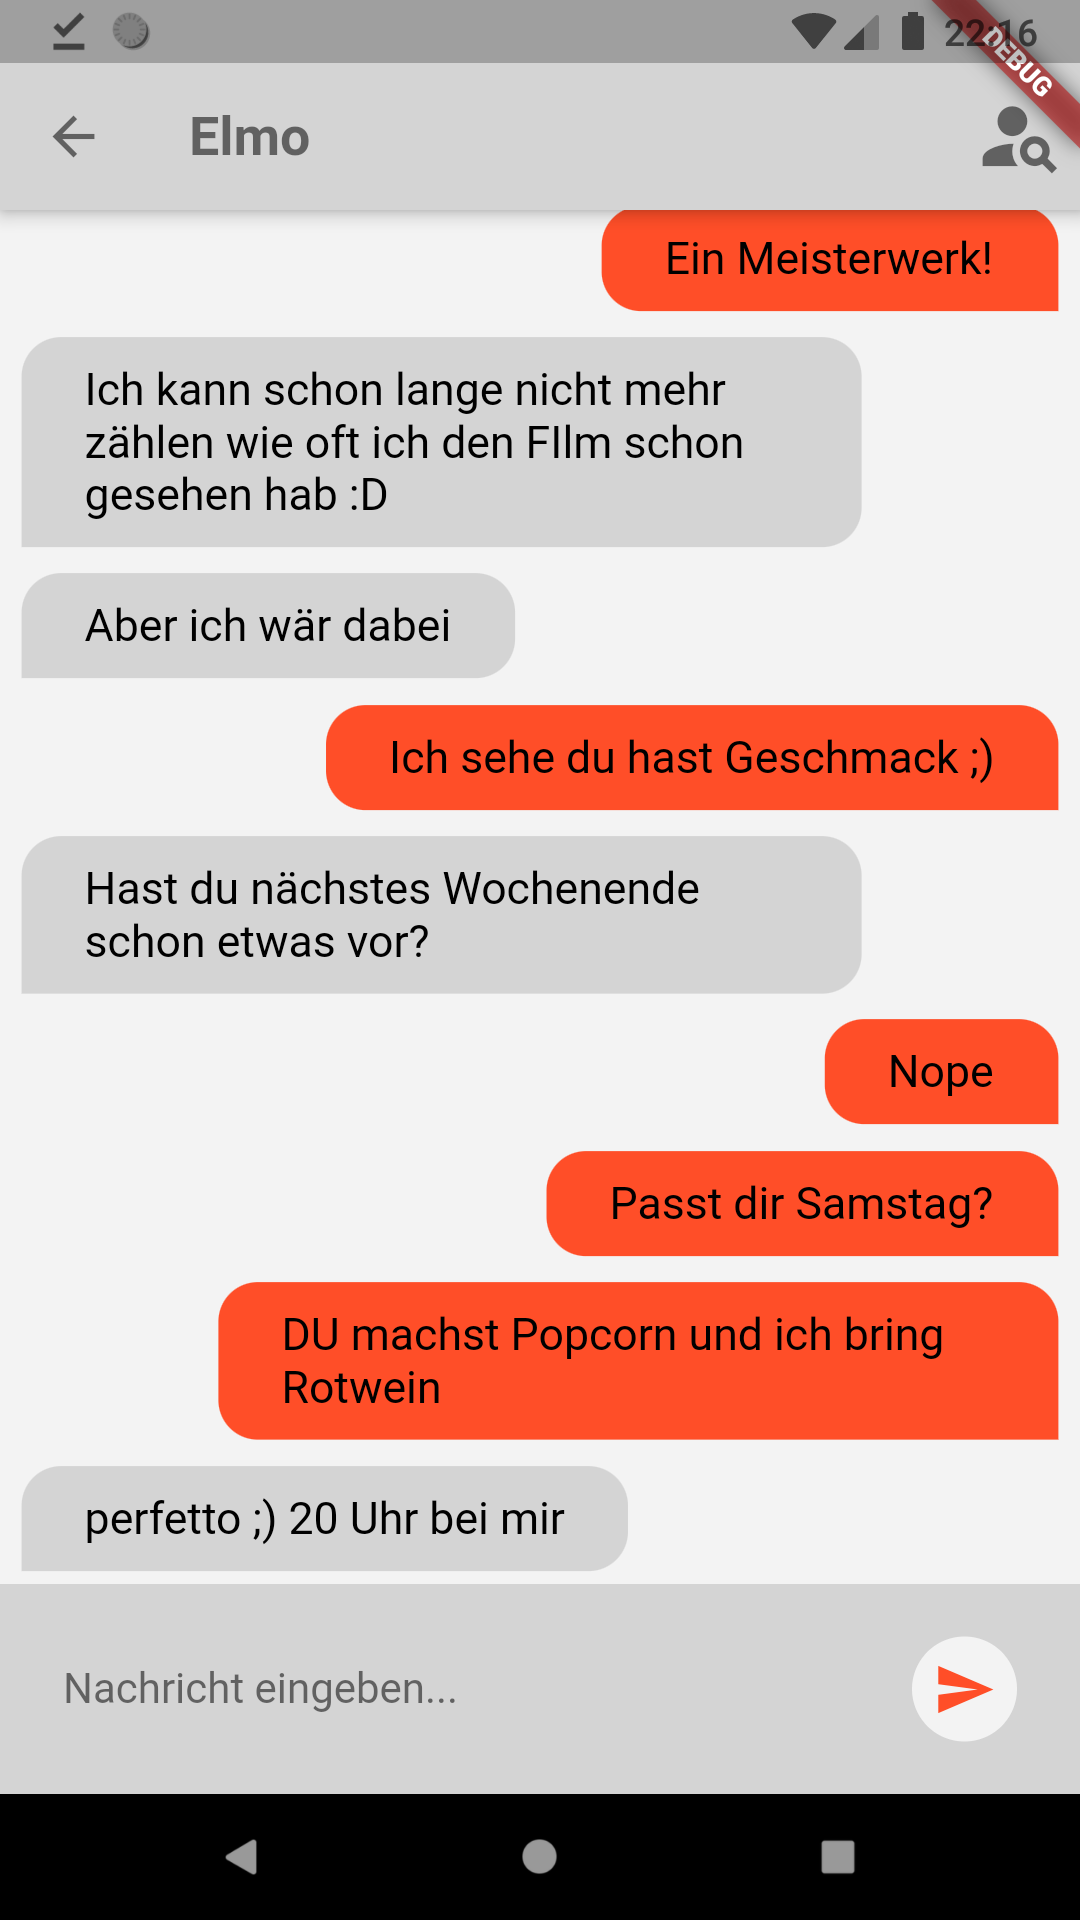
\includegraphics[scale=0.13]{Benutzeroberfläche/images/screenshot_chat_5.png}
	\caption{}
	\label{fig:chat_e}
	\end{subfigure}
	\begin{subfigure}{0.33\textwidth}
	\centering
	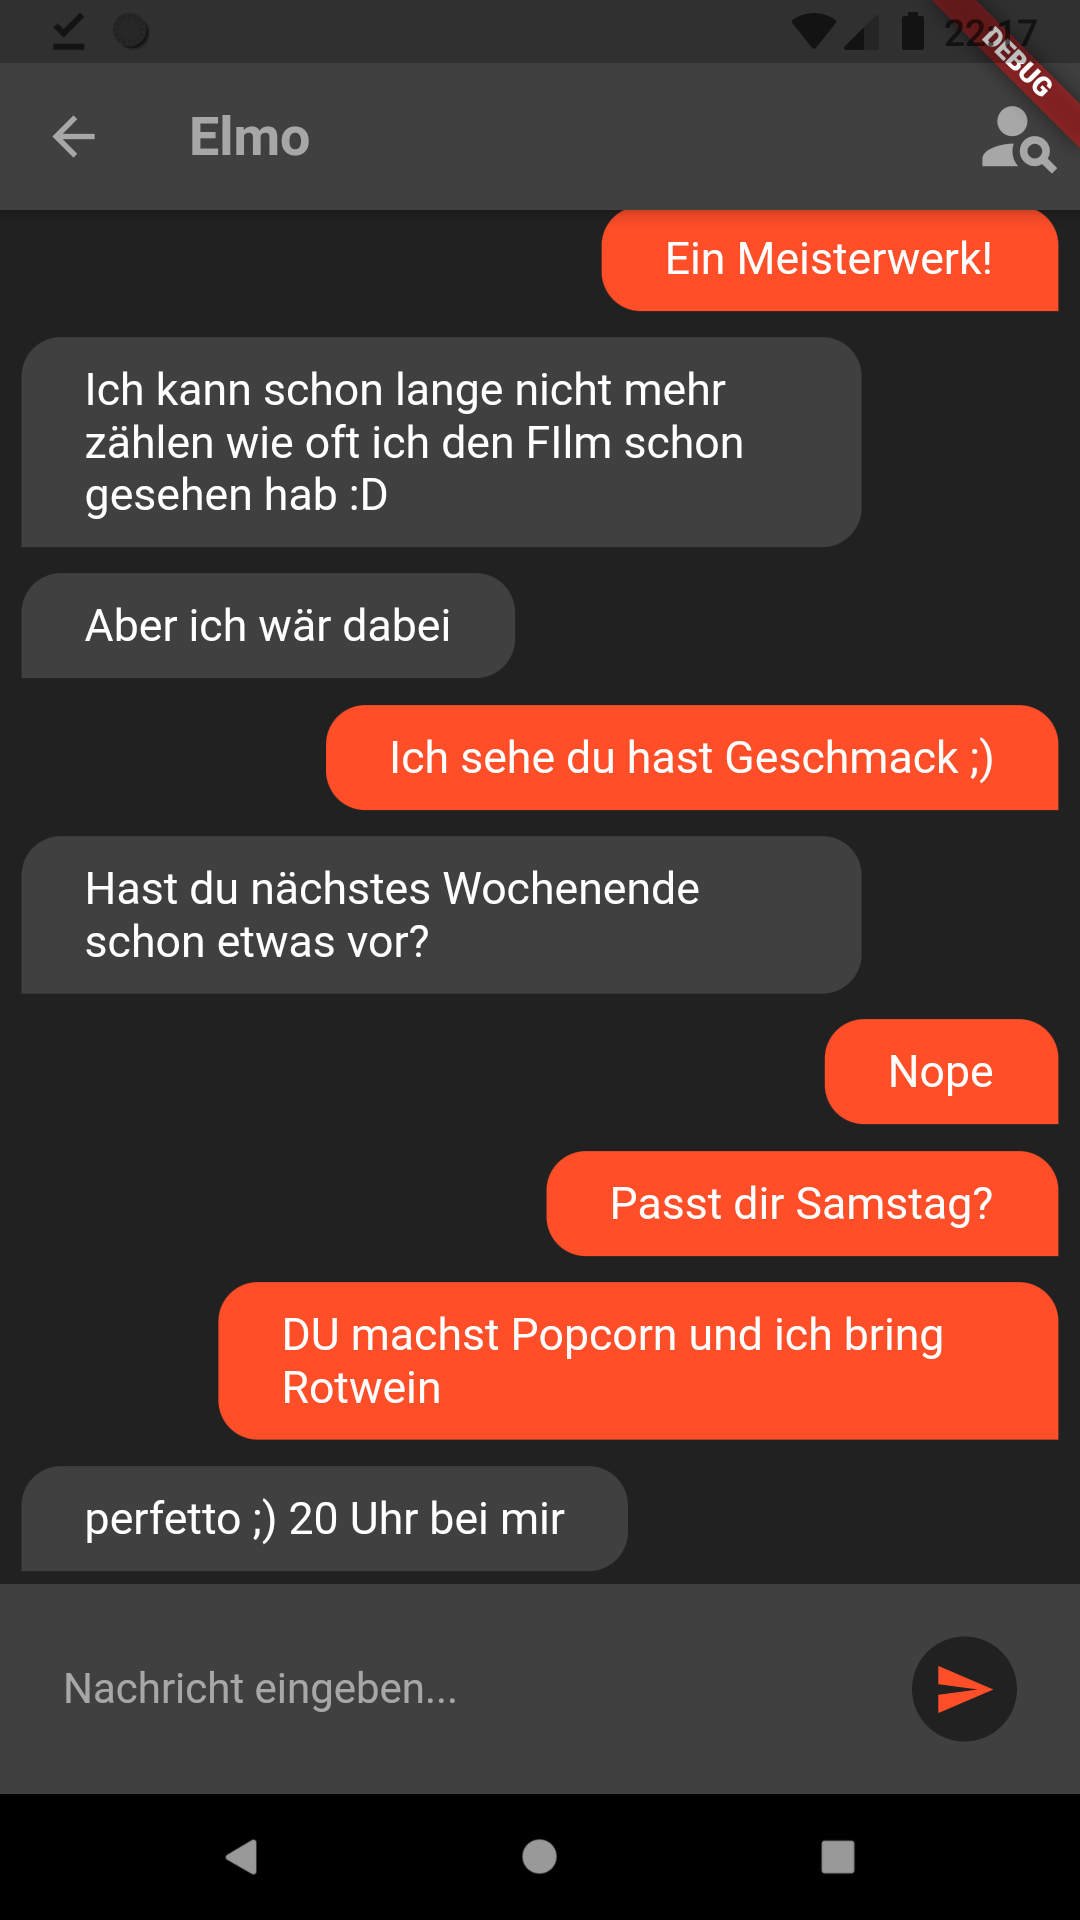
\includegraphics[scale=0.13]{Benutzeroberfläche/images/screenshot_darkmode_4.png}
	\caption{}
	\label{fig:chat_f}
	\end{subfigure}
\caption[Screenshots der Chat-Seiten]{Darstellungen und Funktionen der Chat-Screens mit (a) den aktiven Chats, (b) den Chats auf der Warteliste, (c) und (d) angenommene, bzw. abgelehnten Chats auf der Warteliste, sowie (e) einem Chatverlauf im hellen und (f) in dunklen Modus.}
\label{fig:chat_alle}
\end{figure}



\subsubsection{Benutzerprofil}
\label{sec:benutzerprofil}

Auf der Profilseite werden ein Profilbild, ein Hintergrundbild und für das Matching relevante persönliche Informationen dargestellt. Es gibt eine Version, die nur von anderen Nutzern sichtbar ist, mit denen ein Match stattgefunden hat, und eine Version, die über die Bottom-Navigation-Bar erreichbar werden kann. Die Letztere wird in Abbildung \ref{fig:profilseite_alle} dargestellt und unterscheidet sich von der Version für andere Nutzer darin, dass Profil- und Hintergrundbild bearbeitet werden können.\\
Das Farbschema und das Design wurden an die bisherigen Seiten angepasst. Um die Oberfläche simpel und selbsterklärend zu halten, wird jede dargestellte Information mit einem passenden Icon und einem Hinweis versehen (siehe Abbildung \ref{fig:profilseite_a}). Die Icons zum Bearbeiten der Bilder sind, wie auch in vielen anderen Apps, platziert und designt. Sie öffnen die systemeigene Bildergalerie des Smartphones um den Nutzer aus einem bekannten Umfeld Bilder auswählen lassen zu können.\\
Beim initialen Öffnen einer Profilseite sollen Namen, Profilbild und ein Hintergrundbild ins Auge springen. Sie stellen die ersten Informationen dar, die dem Betrachter wichtig sind, weshalb sie wie in Abbildung \ref{fig:profilseite_a} deutlich sichtbar ist  beim Öffnen mehr als die Hälfte des Bildschirms einnehmen. Anschließend wird der Fokus auf detailliertere Informationen gerichtet. Auf der Profilseite von StreamSwipe wird hierfür heruntergescrollt um den Block mit den Profildaten sehen zu können. Bei dieser Aktion blendet eine Animation das Profilbild aus und verschmälert das Hintergrundbild. Der Benutzername wird ebenfalls aus dem Fokus gezogen, bleibt aber wie in Abbildung \ref{fig:profilseite_b} zu sehen mit dem verbleibenden Hintergrundbildausschnitt erhalten. Dies hilft dem Betrachter unterbewusst bei dem Fokuswechsel und schafft ein modernes, responsives Feedback bei der User Experience.\\
Um das durchgängig schlichte Design der App zu erhalten ist der Zugang zu den Einstellungen ausschließlich auf der Profilseite zu finden. Hierfür ist im rechten oberen Bildschirmbereich das repräsentative Icon. Der hierdurch erreichbare Bildschirm (Abbildung \ref{fig:profilseite_c}) ist gleich aufgebaut wie die Informationeneingabe nachdem ein neuer Account erstellt wurde (Abbildungen \ref{fig:login_c} und \ref{fig:login_d}). Die dort angegebenen Informationen können hier wieder angepasst werden. %TODO Referenz auf account erstellen bild


\begin{figure}[tbt]
	\begin{subfigure}{0.33\textwidth}
	\centering
	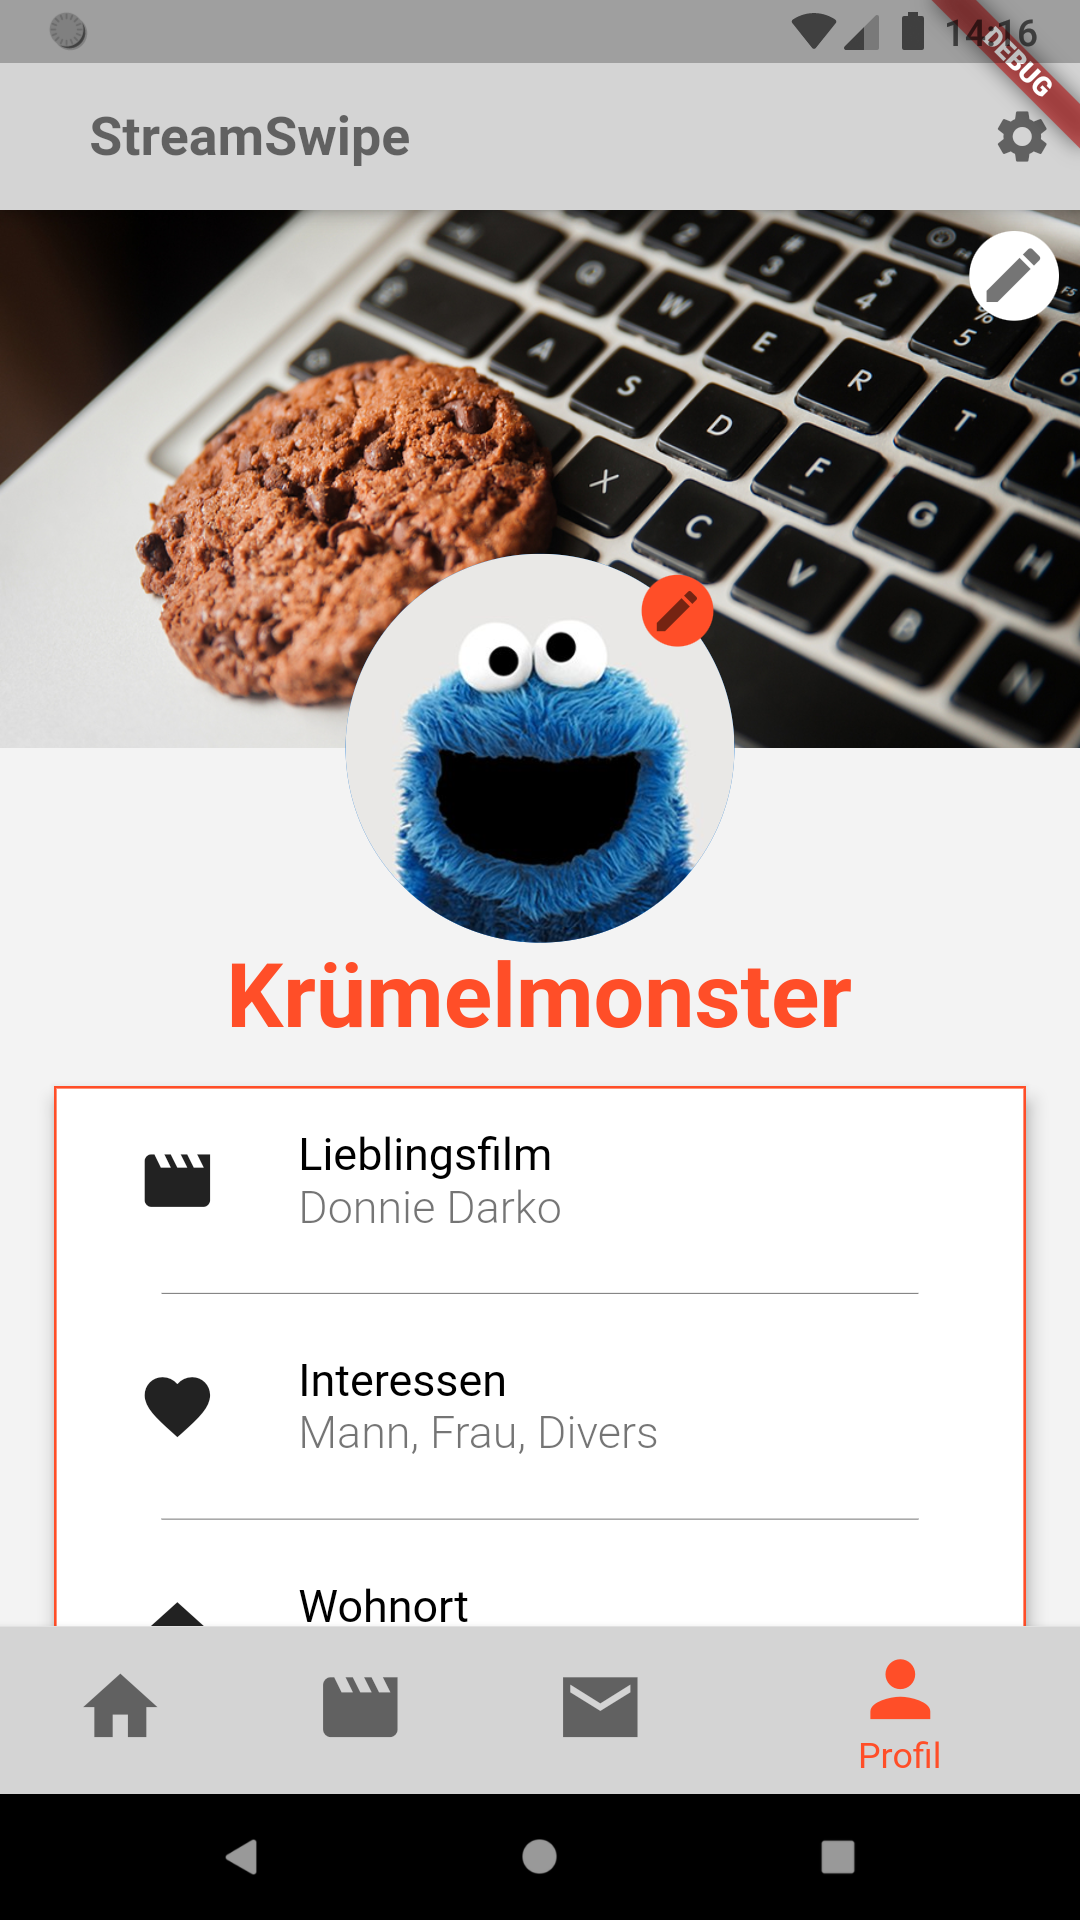
\includegraphics[scale=0.13]{Benutzeroberfläche/images/screenshot_profilseite_1.png}
	\caption{}
	\label{fig:profilseite_a}
	\end{subfigure}
	\begin{subfigure}{0.33\textwidth}
	\centering
	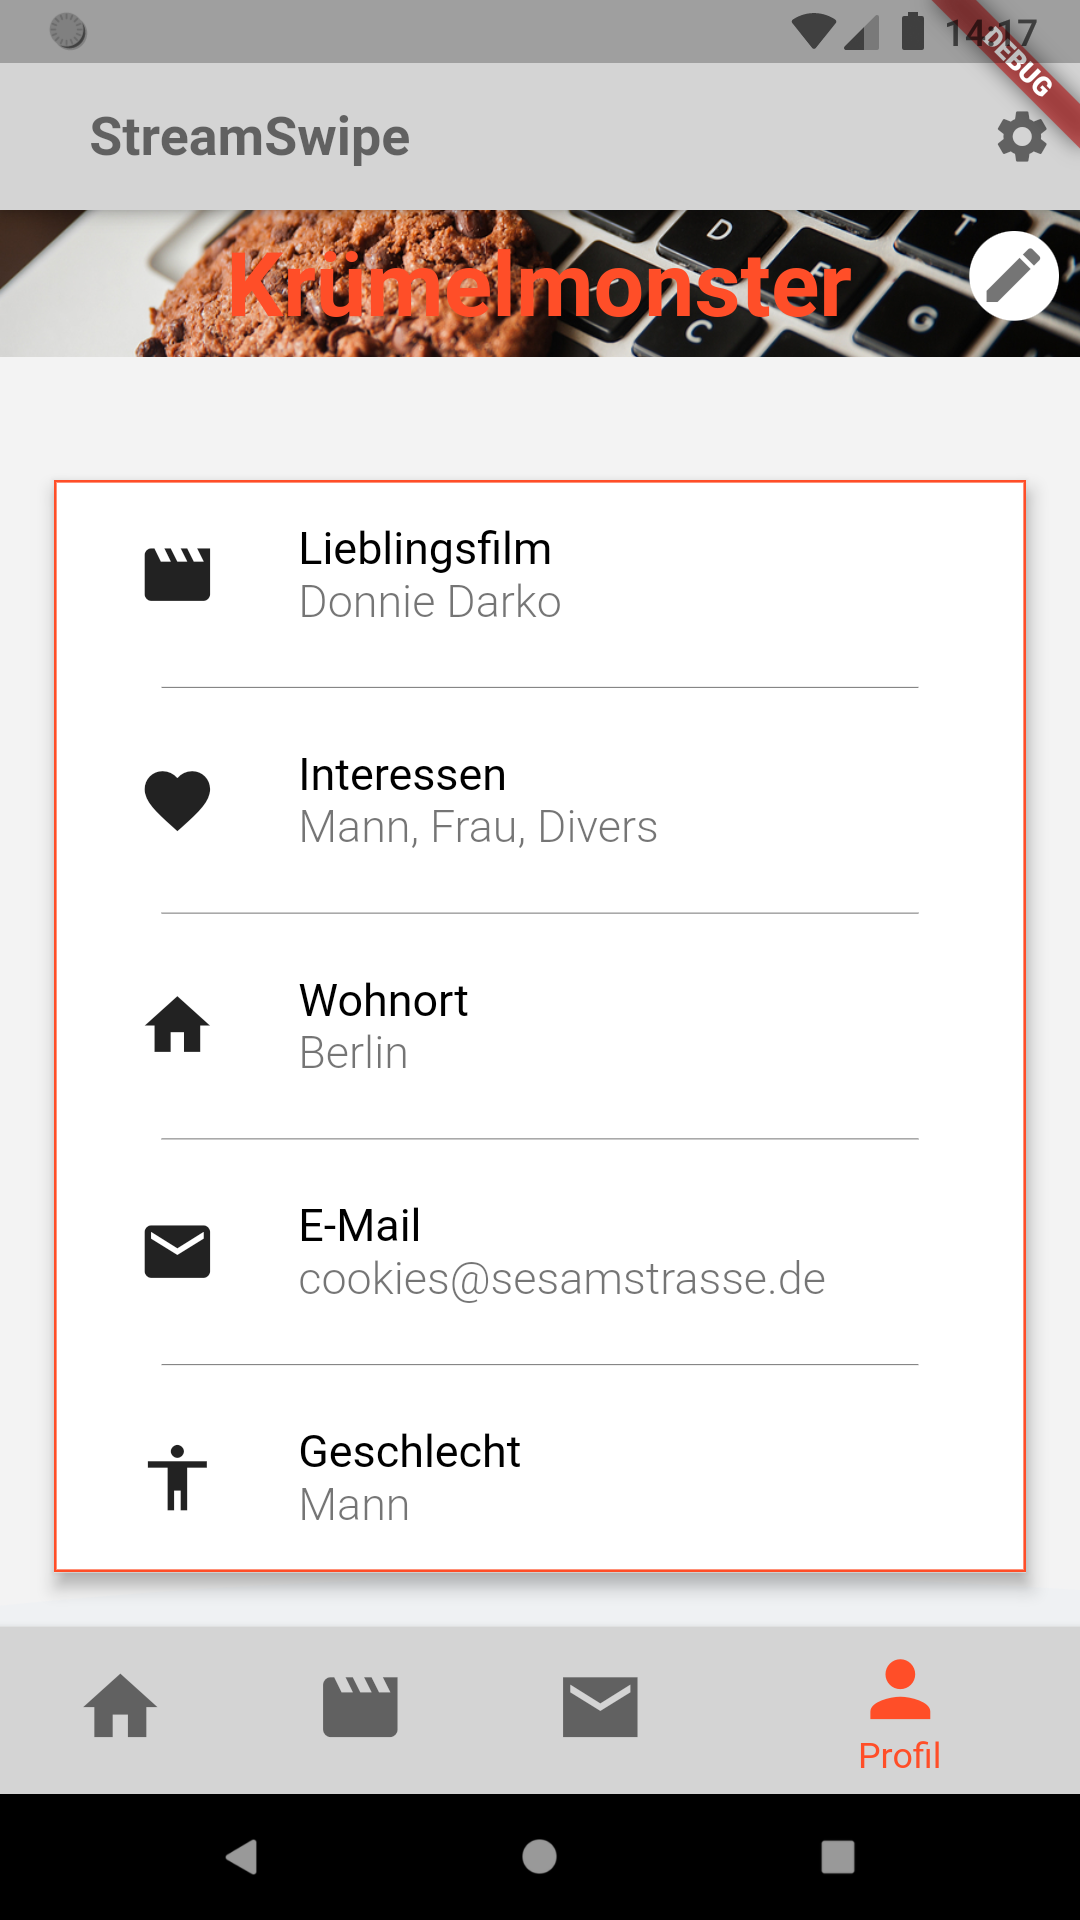
\includegraphics[scale=0.13]{Benutzeroberfläche/images/screenshot_profilseite_2.png}
	\caption{}
	\label{fig:profilseite_b}
	\end{subfigure}
	\begin{subfigure}{0.33\textwidth}
	\centering
	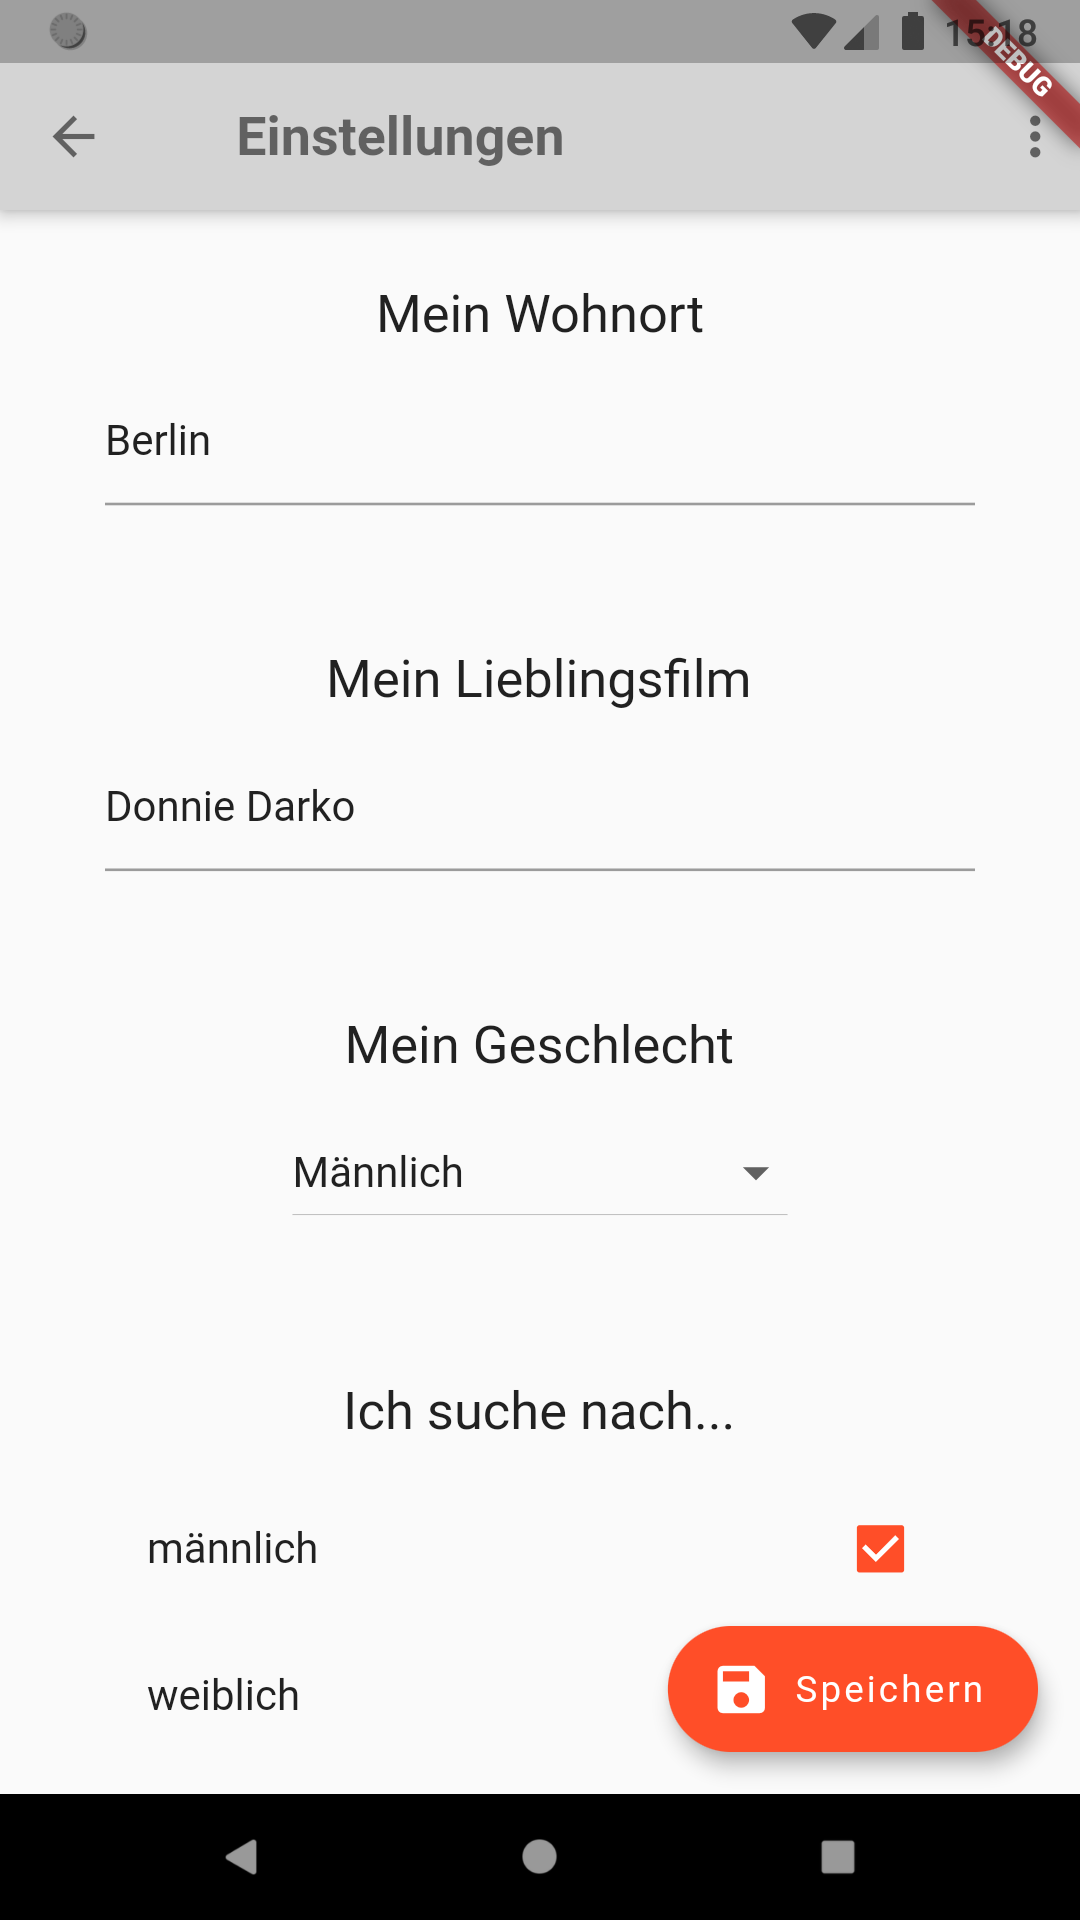
\includegraphics[scale=0.13]{Benutzeroberfläche/images/screenshot_profilseite_3}
	\caption{}
	\label{fig:profilseite_c}
	\end{subfigure}
\caption[Screenshots der Profilseite]{Profilseite wie sie für den Nutzer selbst angezeigt wird (a) im normalen Zustand und (b) nach vollständigem Einklappen des Profilkopfes durch eine Animation während dem Herunterscrollen. Mit den von hier aus erreichbaren Einstellungen (c) können die anfänglich gegebenen Profilangaben abgepasst werden.}
\label{fig:profilseite_alle}
\end{figure}



\subsection{Filmliste}


\section[CodeBeispiele]{CodeBeispiele \hfill \normalfont \small{Autor-Name}}


\section[Probleme]{Probleme \hfill \normalfont \small{Autor-Name}}


\section[Fazit]{Fazit \hfill \normalfont \small{Autor-Name}}


\section{Literaturverzeichnis}
\begin{itemize}
\bibitem[1]{scheidungen} Meinungsforschungsinstituts Civey (2020):  \url{https://www.presseportal.de/pm/145489/4627304}, letzter Zugriff: 13. Mai 2021
\bibitem[1]{serienkonsum} Splendid Research (2017): \url{https://www.springerprofessional.de/konsumforschung/marketingstrategie/konsumenten-auf-der-serien-welle/15146374}, letzter Zugriff: 14. Mai 2021
\bibitem[1]{schwerbehindertenausweis} Statistisches Bundesamt (2020): \url{https://www.destatis.de/DE/Themen/Gesellschaft-Umwelt/Gesundheit/Behinderte-Menschen/Tabellen/schwerbehinderte-alter-geschlecht-quote.html;jsessionid=885260788D4FFC7F670576B72E5089F4.live741}, letzter Zugriff: 17. April 2021
\bibitem[2]{behindertengleichstellungsgesetz} Behindertengleichstellungsgesetz (2002): \url{https://www.gesetze-im-internet.de/bgg/BGG.pdf}, letzter Zugriff: 19. April 2021
\bibitem[3]{sehhilfen} Institut für Demoskopie Allensbach (2019): \textit{Untersuchung zum Sehbewusstsein der Deutschen},  \url{file:///C:/Users/Vincent/AppData/Local/Temp/ZVA_Brillenstudie_2019-1.pdf}, letzter Zugriff: 11. Mai 2021


\bibitem[99]{muster} Mustermann, Max (2020): Methode und Nutzung der Literatur-Zitierweise, 2. Aufl., Boston: Harvard’s Eleven Publications.
\bibitem[99]{asdf} Autor (2008): Name des Buches, 22. Aufl., Berlin: Foxtrott.
\end{itemize}


\end{document}



\footnote{\url{https://de.wikipedia.org/wiki/Alufolie}} 


Abbildung \ref{fig:allg_kennlinie}

\begin{figure}[tbt]
\begin{center}
\includegraphics[scale=0.45]{Grafiken/allg_kennlinie.png}
\end{center}
\caption{Kennlinie einer Halbleiterdiode \protect \footnotemark}
\label{fig:allg_kennlinie}
\end{figure}
\footnotetext{FUSSNOTE}


Tabelle \ref{tab:cobalt}

\begin{table}[tbt]
\caption{•}
\begin{threeparttable}	%Scheme for footnotes in tables
\begin{center}
\begin{tabular}{c c c c}
\toprule
& keV & keV & keV \\
\midrule
a	& b	& c	& d \\
a	& b	& c	& d \\
a	& b	& c	& d \\
a	& b	& c	& d \\ %direkt hinter jeweiligen Wert /tnote{1}
\bottomrule
\end{tabular}
\end{center}
\begin{tablenotes}\footnotesize 
\item[1]{Quelle: http://www.thinksrs.com/downloads/PDFs/ApplicationNotes/IG1BAgasapp.pdf}
\end{tablenotes}
\end{threeparttable}
\label{tab:cobalt}
\end{table}